\section{Model study}

This section compares six model families under a strictly common experimental framework. The primary metric is \texttt{F1-macro}, selected to give equal weight to all \texttt{99} species, while \texttt{accuracy} serves as the secondary metric.

The analysis follows three clearly distinguished levels of evidence. Exploratory variants use simple cross-validation to measure the effects of preprocessing or complexity control. The primary result for each family is the \texttt{tuned} variant, evaluated through nested cross-validation. When available, secondary corroboration on the frozen split is used solely to determine whether the signal observed on the development set persists on data never seen during modeling.

The following subsections share a common structure. Each model is first situated within the scientific rationale of the study, then examined from exploratory, confirmatory, and, where available, secondary corroboration perspectives.

The purpose of this section is not yet to reach an overall verdict among models, but to understand how each family responds to preprocessing, complexity control, and tuning. The cross-model synthesis is deliberately reserved for the next section to maintain a clear separation between family-specific analysis and the final comparative assessment.

% --- PERCEPTRON ---
\subsection{Perceptron model}

\subsubsection{Role of the model}
The perceptron is the study's minimal linear baseline. Its purpose is less to compete with the best models than to quantify what an elementary decision boundary can extract from a high-dimensional multiclass problem. It therefore provides a useful reference point for measuring the effect of standardization and, more generally, the need for additional model capacity.

\subsubsection{Exploration}
The exploratory stage immediately shows that preprocessing plays a central role for this family. The raw variant achieves a \texttt{F1-macro} of \texttt{0.6979} and an \texttt{accuracy} of \texttt{0.7436}. Adding \texttt{StandardScaler} raises \texttt{F1-macro} to \texttt{0.8228}, while the \texttt{scaled\_pca} variant reaches \texttt{0.8057}. The main gain therefore comes from scaling; dimensionality reduction provides no additional robust improvement here.

\begin{table}[H]
\centering
\begin{tabular}{|l|l|r|r|r|r|}
\hline
\textbf{Variant} & \textbf{Protocol} & \textbf{Macro F1} & \textbf{Accuracy} & \textbf{F1 gap} & \textbf{Time (s)} \\
\hline
\texttt{default} & simple CV & \texttt{0.6979} & \texttt{0.7436} & \texttt{0.1202} & \texttt{0.62} \\
\texttt{scaled\_only} & simple CV & \texttt{0.8228} & \texttt{0.8460} & \texttt{0.1732} & \texttt{0.60} \\
\texttt{scaled\_pca} & simple CV & \texttt{0.8057} & \texttt{0.8346} & \texttt{0.1923} & \texttt{0.65} \\
\hline
\end{tabular}
\caption{Comparison of perceptron variants}
\end{table}

The perceptron therefore becomes substantially more credible after normalization, but the size of the generalization gap indicates that its room for improvement remains limited. This exploratory evidence already suggests that a low-capacity, non-probabilistic linear model will serve more as a lower bound than as a leading candidate.

\begin{figure}[H]
\centering
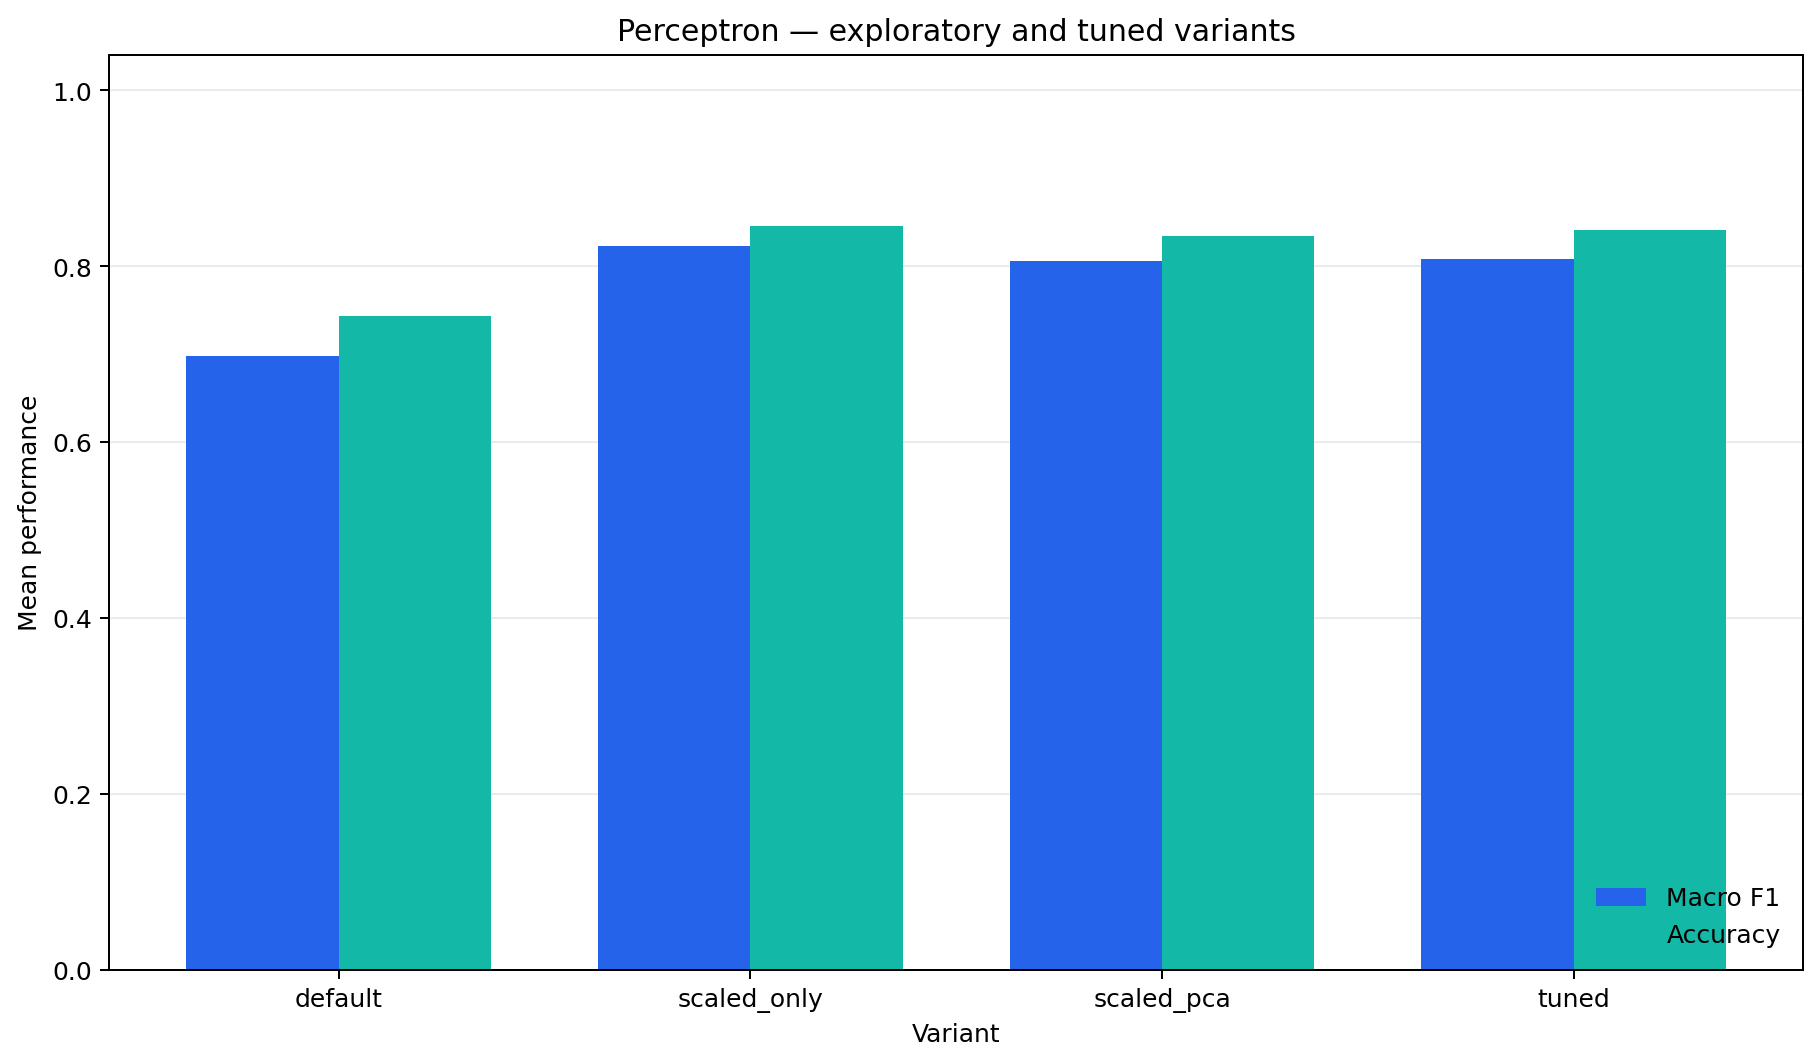
\includegraphics[width=\textwidth]{../figures/en/figA2b_comparaison_perceptron.png}
\caption{Exploratory comparison of perceptron variants. Nearly the entire performance increase is explained by feature standardization.}
\end{figure}

\subsubsection{Confirmation}
Confirmatory evaluation through nested cross-validation yields a mean \texttt{F1-macro} of \texttt{0.8085} and mean \texttt{accuracy} of \texttt{0.8409}, with standard deviations of \texttt{0.0523} and \texttt{0.0411}. The confirmatory score remains slightly below that of the best exploratory variant (\texttt{scaled\_only}), which is consistent with a less optimistic estimate after model selection.

\begin{table}[H]
\centering
\begin{tabular}{|l|r|}
\hline
\textbf{Confirmatory metric} & \textbf{Value} \\
\hline
Mean Macro F1 & \texttt{0.8085} \\
F1 standard deviation & \texttt{0.0523} \\
Mean accuracy & \texttt{0.8409} \\
Accuracy standard deviation & \texttt{0.0411} \\
Protocol & \texttt{nested CV} \\
Outer folds & \texttt{5} \\
Inner folds & \texttt{3} \\
Total time (s) & \texttt{29.79} \\
\hline
\end{tabular}
\end{table}

The scientific conclusion remains stable: once the variables are standardized, the perceptron captures a substantial part of the problem's structure, but still lags well behind the strongest families. It therefore fully serves its role as a minimal linear baseline without becoming a credible contender for the final ranking.

\subsubsection{Descriptive diagnostics}
The figures associated with the perceptron are primarily descriptive. The decision-function histogram shows the dispersion of margin scores, while the confusion matrix and leading-confusion summary show that residual errors remain relatively diffuse. This pattern is consistent with the limitations of a simple linear boundary on a problem with \texttt{99} classes.

\begin{figure}[H]
\centering
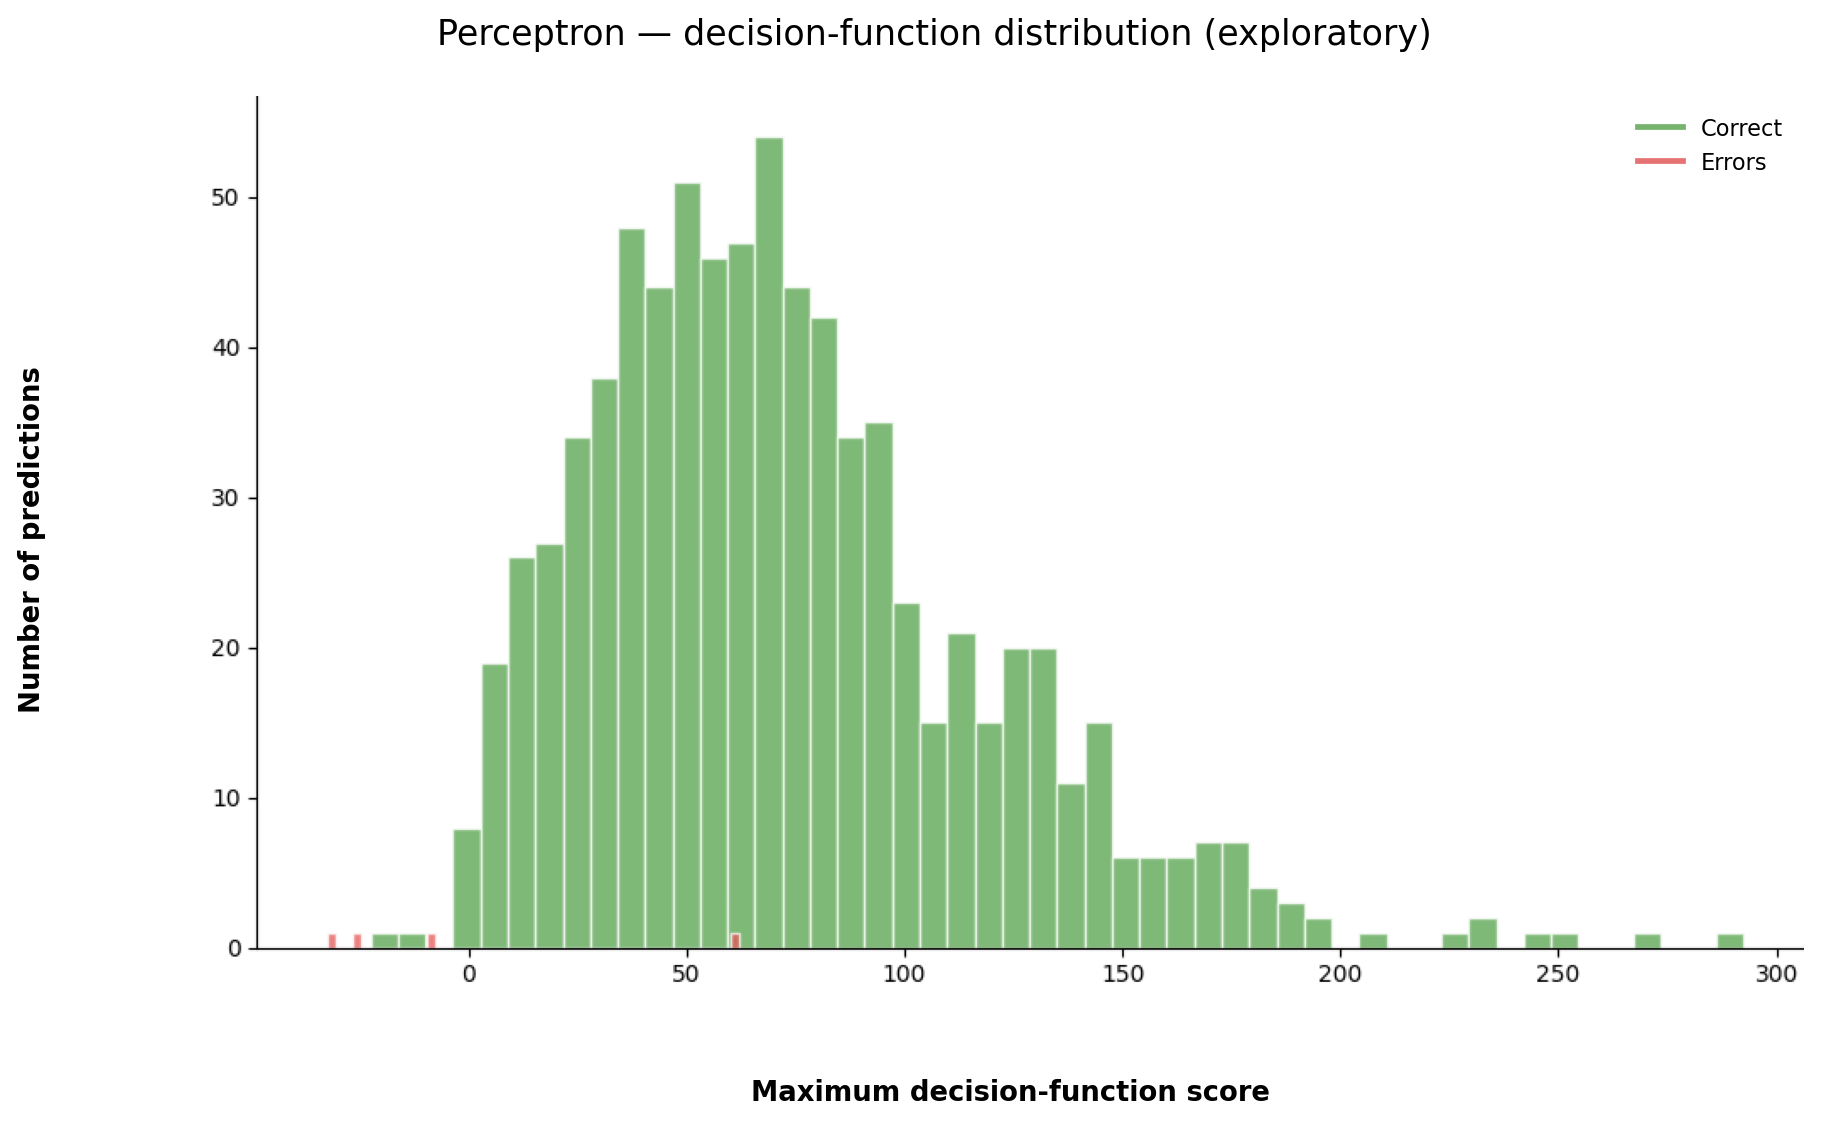
\includegraphics[width=\textwidth]{../figures/en/fig_perceptron_histogramme_fonction_decision.png}
\caption{Exploratory histogram of the perceptron's decision function. The score dispersion is consistent with a useful but still limited linear separation.}
\end{figure}

\begin{figure}[H]
\centering
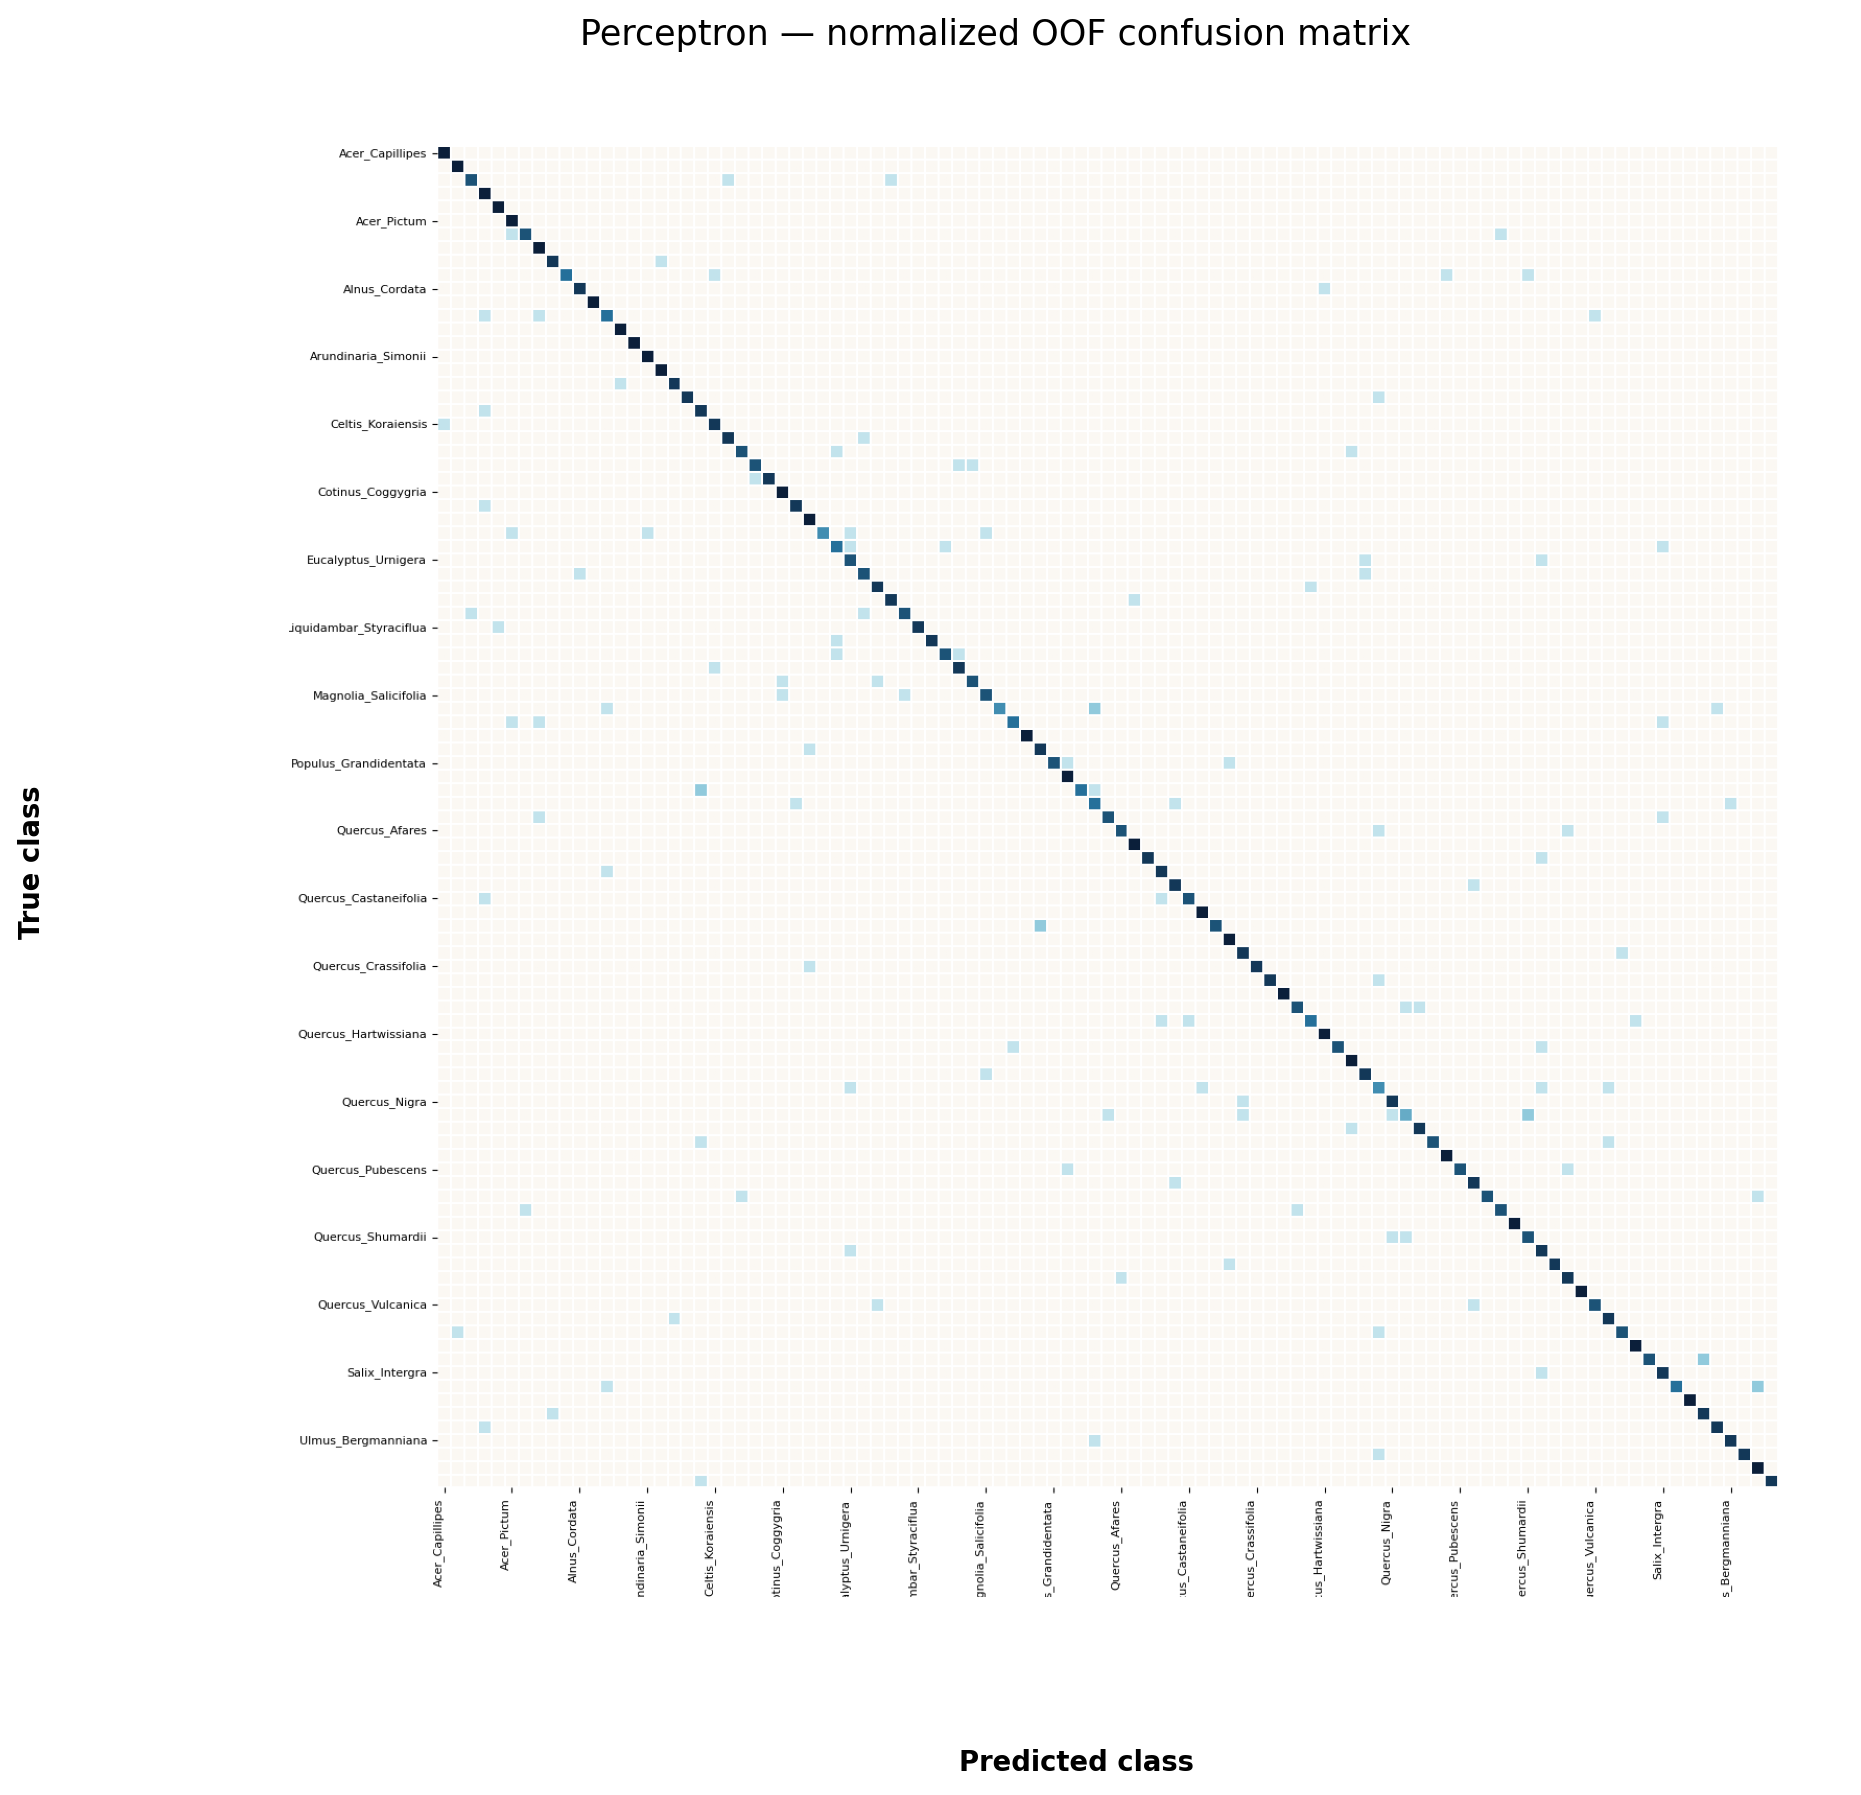
\includegraphics[width=\textwidth]{../figures/en/figA_confusion_perceptron_tuned.png}
\caption{Normalized confusion matrix obtained from the out-of-fold predictions of the \texttt{tuned} variant. Residual errors remain more diffuse than for the best-performing families.}
\end{figure}

\begin{figure}[H]
\centering
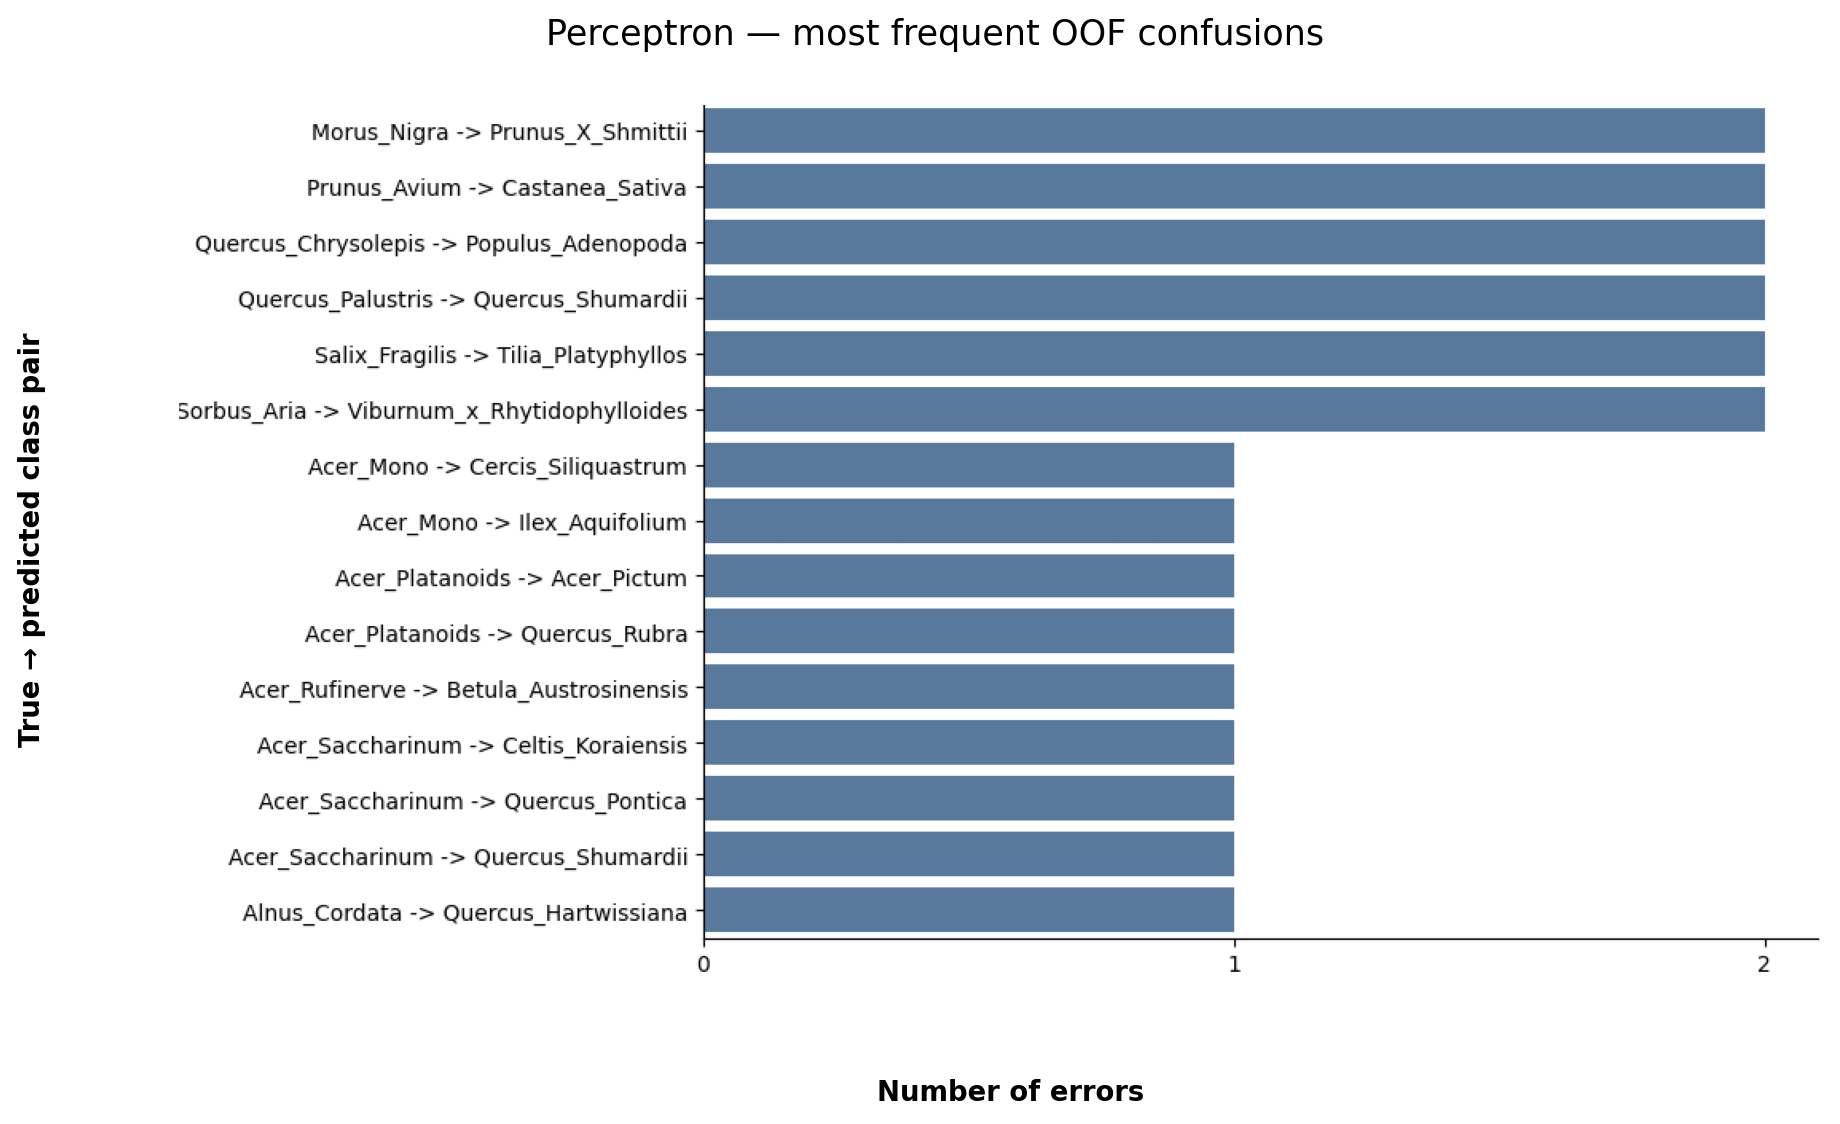
\includegraphics[width=\textwidth]{../figures/en/fig_perceptron_top12_confusions.png}
\caption{Leading confusions observed for the tuned perceptron. Their dispersion confirms that the model remains limited by its separation capacity.}
\end{figure}

\subsubsection{Secondary corroboration}
Secondary corroboration is available on the frozen split. The reference variant is \texttt{scaled\_only}, selected from the exploratory results on the development set. On the corroboration set, this reference achieves a \texttt{F1-macro} of \texttt{0.8815}, compared with \texttt{0.8694} for the \texttt{tuned} variant. The \texttt{tuned - reference} delta is therefore \texttt{-0.0121}.

\begin{table}[H]
\centering
\begin{tabular}{|l|r|r|l|}
\hline
\textbf{Variant} & \textbf{Corroboration F1} & \textbf{Corroboration accuracy} & \textbf{Role} \\
\hline
\texttt{default} & \texttt{0.8318} & \texttt{0.8586} & baseline \\
\texttt{scaled\_only} & \texttt{0.8815} & \texttt{0.8939} & reference \\
\texttt{scaled\_pca} & \texttt{0.8671} & \texttt{0.8838} & descriptive \\
\texttt{tuned} & \texttt{0.8694} & \texttt{0.8838} & tuned \\
\hline
\end{tabular}
\end{table}

For the perceptron, corroboration primarily confirms that the useful gain comes from standardization. Tuning provides no robust improvement for this inflexible family, which therefore remains chiefly an informative linear baseline.

\begin{figure}[H]
\centering
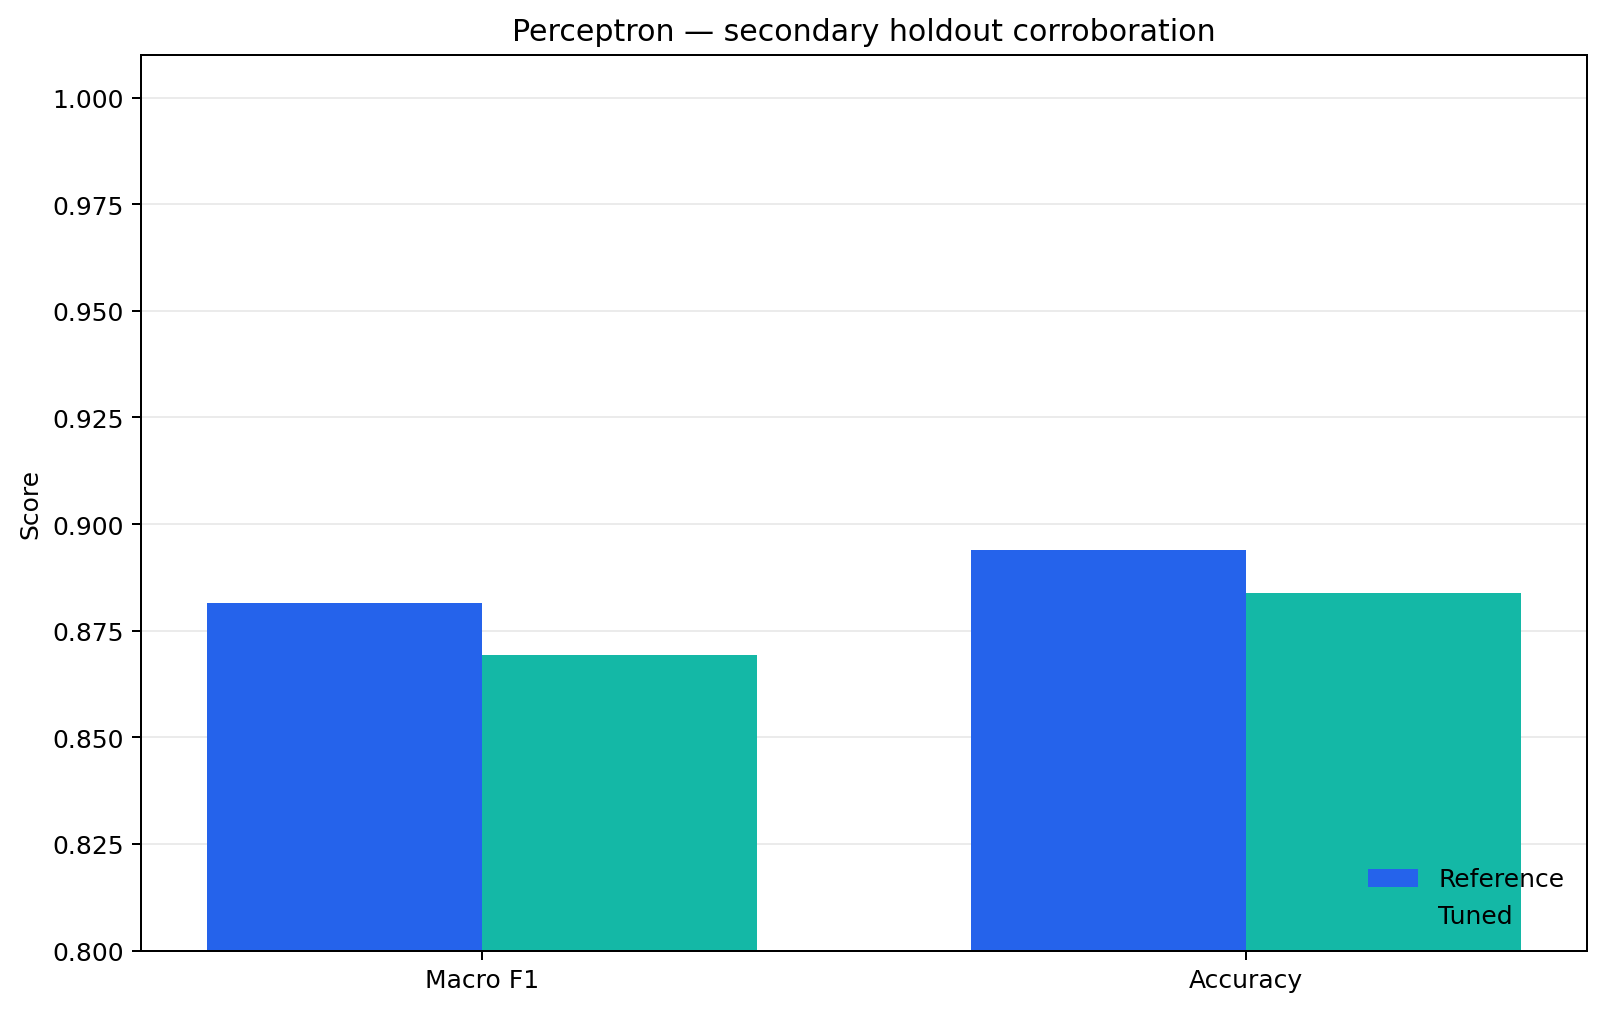
\includegraphics[width=\textwidth]{../figures/en/fig_perceptron_corroboration_holdout.png}
\caption{Secondary comparison between the reference and \texttt{tuned} perceptron variants on the corroboration set.}
\end{figure}

% --- LOGISTIC REGRESSION ---
\subsection{Logistic regression model}

\subsubsection{Role of the model}
Logistic regression is the project's probabilistic linear reference. It combines a simple decision structure, controlled regularization, and interpretable probabilities, making it a particularly strong anchor for assessing both predictive performance and the quality of probabilistic outputs.

\subsubsection{Exploration}
The exploratory results reveal a very strong dependence on scaling. Without preprocessing, logistic regression reaches only \texttt{0.2591} in \texttt{F1-macro} and \texttt{0.3106} in \texttt{accuracy}. With \texttt{StandardScaler}, it rises to \texttt{0.9798} in \texttt{F1-macro} and \texttt{0.9861} in \texttt{accuracy}. The \texttt{scaled\_pca} variant remains almost level with it (\texttt{0.9784} in \texttt{F1-macro}), with no robust gain over scaling alone.

\begin{table}[H]
\centering
\begin{tabular}{|l|l|r|r|r|r|}
\hline
\textbf{Variant} & \textbf{Protocol} & \textbf{Macro F1} & \textbf{Accuracy} & \textbf{F1 gap} & \textbf{Time (s)} \\
\hline
\texttt{default} & simple CV & \texttt{0.2591} & \texttt{0.3106} & \texttt{0.0899} & \texttt{1.69} \\
\texttt{scaled\_only} & simple CV & \texttt{0.9798} & \texttt{0.9861} & \texttt{0.0202} & \texttt{8.10} \\
\texttt{scaled\_pca} & simple CV & \texttt{0.9784} & \texttt{0.9848} & \texttt{0.0216} & \texttt{2.21} \\
\hline
\end{tabular}
\end{table}

This stage already establishes a strong result: on this dataset, a well-regularized linear model becomes extremely effective once supplied with correctly standardized variables. The family therefore immediately emerges as one of the leading candidates in the final ranking.

\begin{figure}[H]
\centering
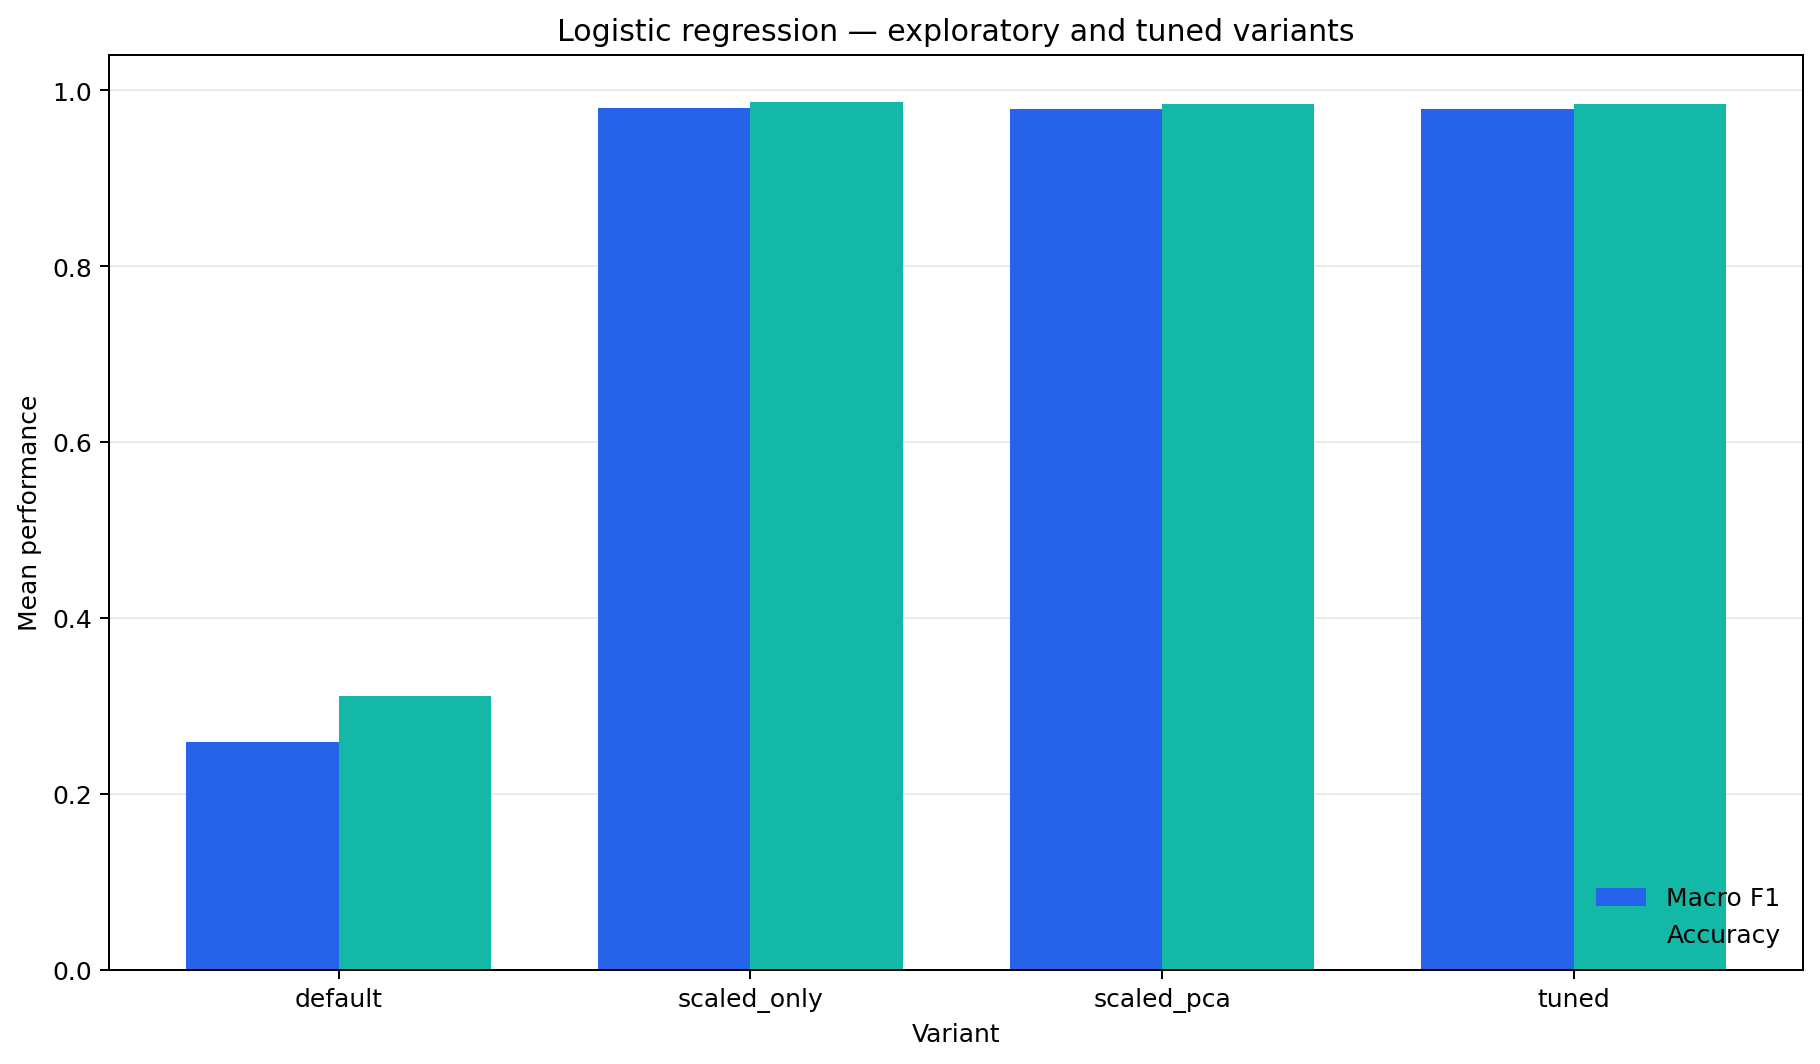
\includegraphics[width=\textwidth]{../figures/en/fig_lr_comparaison_variantes.png}
\caption{Exploratory comparison of logistic-regression variants. Scaling transforms a weak linear model into one of the study's best-performing classifiers.}
\end{figure}

\subsubsection{Confirmation}
Nested cross-validation fully confirms this interpretation. The \texttt{tuned} variant achieves a mean \texttt{F1-macro} of \texttt{0.9787} and mean \texttt{accuracy} of \texttt{0.9848}, with standard deviations of \texttt{0.0198} and \texttt{0.0146}. The confirmatory estimate is virtually identical to that of the best exploratory variant, indicating excellent signal stability.

\begin{table}[H]
\centering
\begin{tabular}{|l|r|}
\hline
\textbf{Confirmatory metric} & \textbf{Value} \\
\hline
Mean Macro F1 & \texttt{0.9787} \\
F1 standard deviation & \texttt{0.0198} \\
Mean accuracy & \texttt{0.9848} \\
Accuracy standard deviation & \texttt{0.0146} \\
Protocol & \texttt{nested CV} \\
Outer folds & \texttt{5} \\
Inner folds & \texttt{3} \\
Total time (s) & \texttt{77.05} \\
\hline
\end{tabular}
\end{table}

Logistic regression leads the confirmatory means and, together with the SVM, forms the report's top pair. Its strength does not come from complex tuning, but from the remarkable fit between linear regularization, standardization, and the structure of the problem.

\subsubsection{Descriptive diagnostics}
The diagnostics for this family help explain why it performs so well. The regularization path shows that performance stabilizes quickly within the useful range of \texttt{C}, suggesting that the data already determine a strong boundary once scaling is applied. The leading residual confusions are also very few relative to the observed performance level.

\begin{figure}[H]
\centering
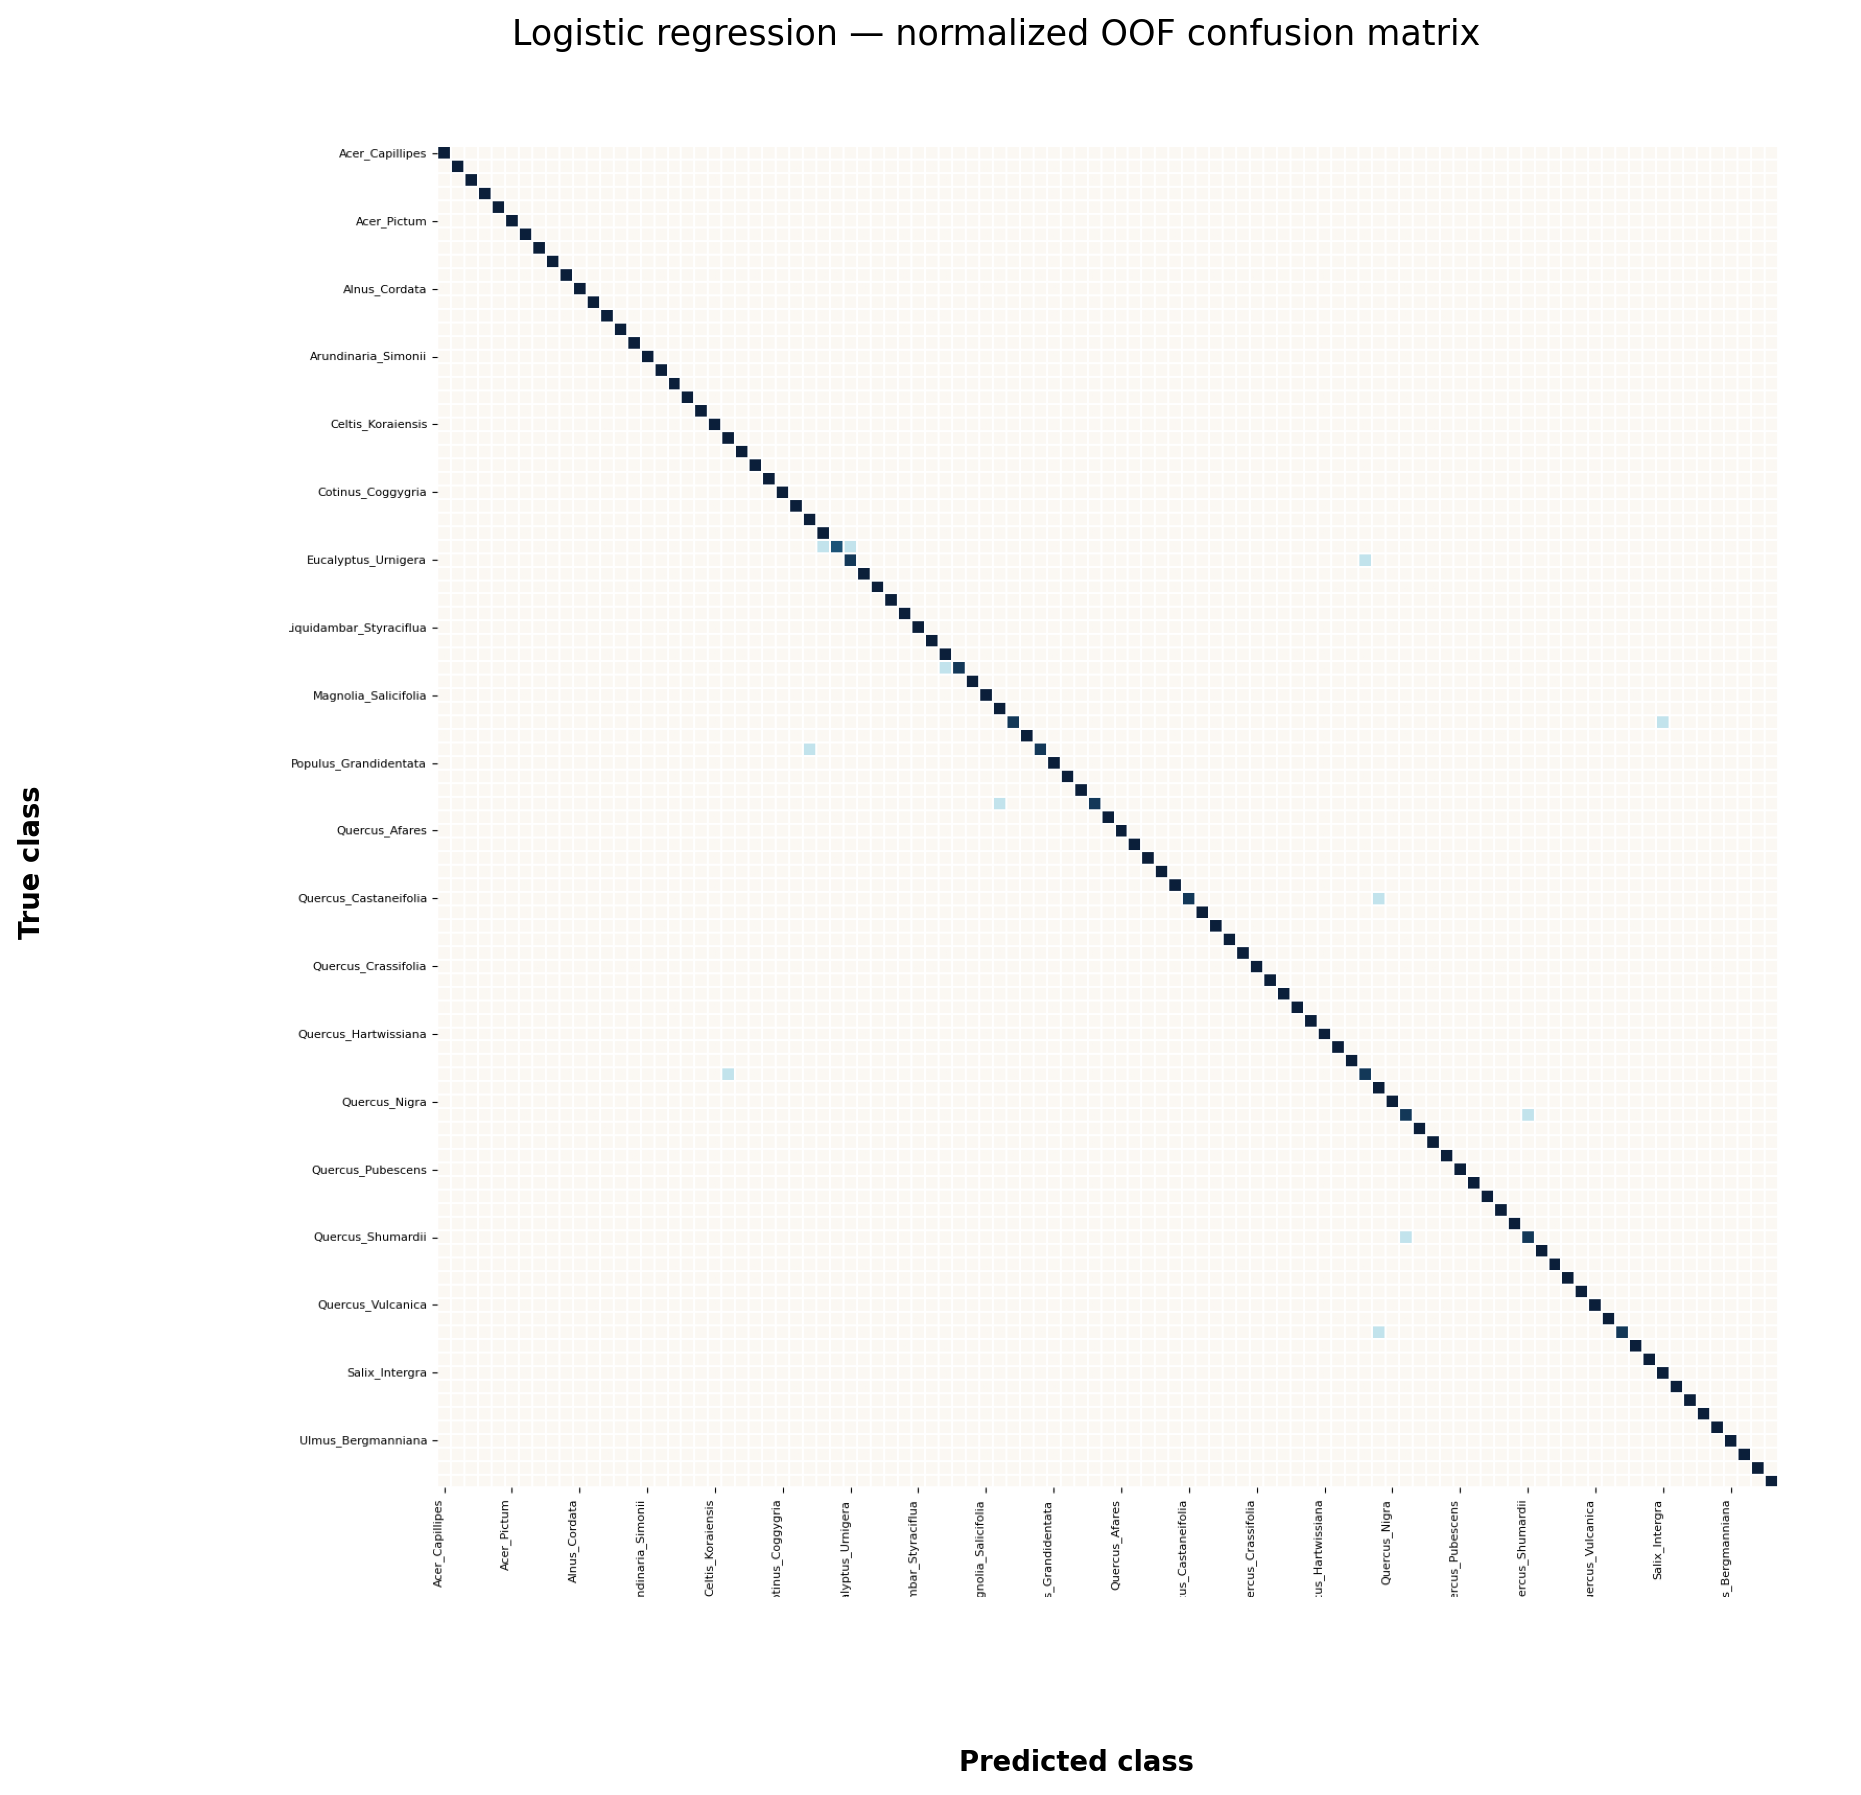
\includegraphics[width=\textwidth]{../figures/en/figA_confusion_lr_tuned.png}
\caption{Normalized confusion matrix from the out-of-fold predictions of the \texttt{tuned} variant. The near-diagonal structure confirms excellent separation among classes.}
\end{figure}

\begin{figure}[H]
\centering
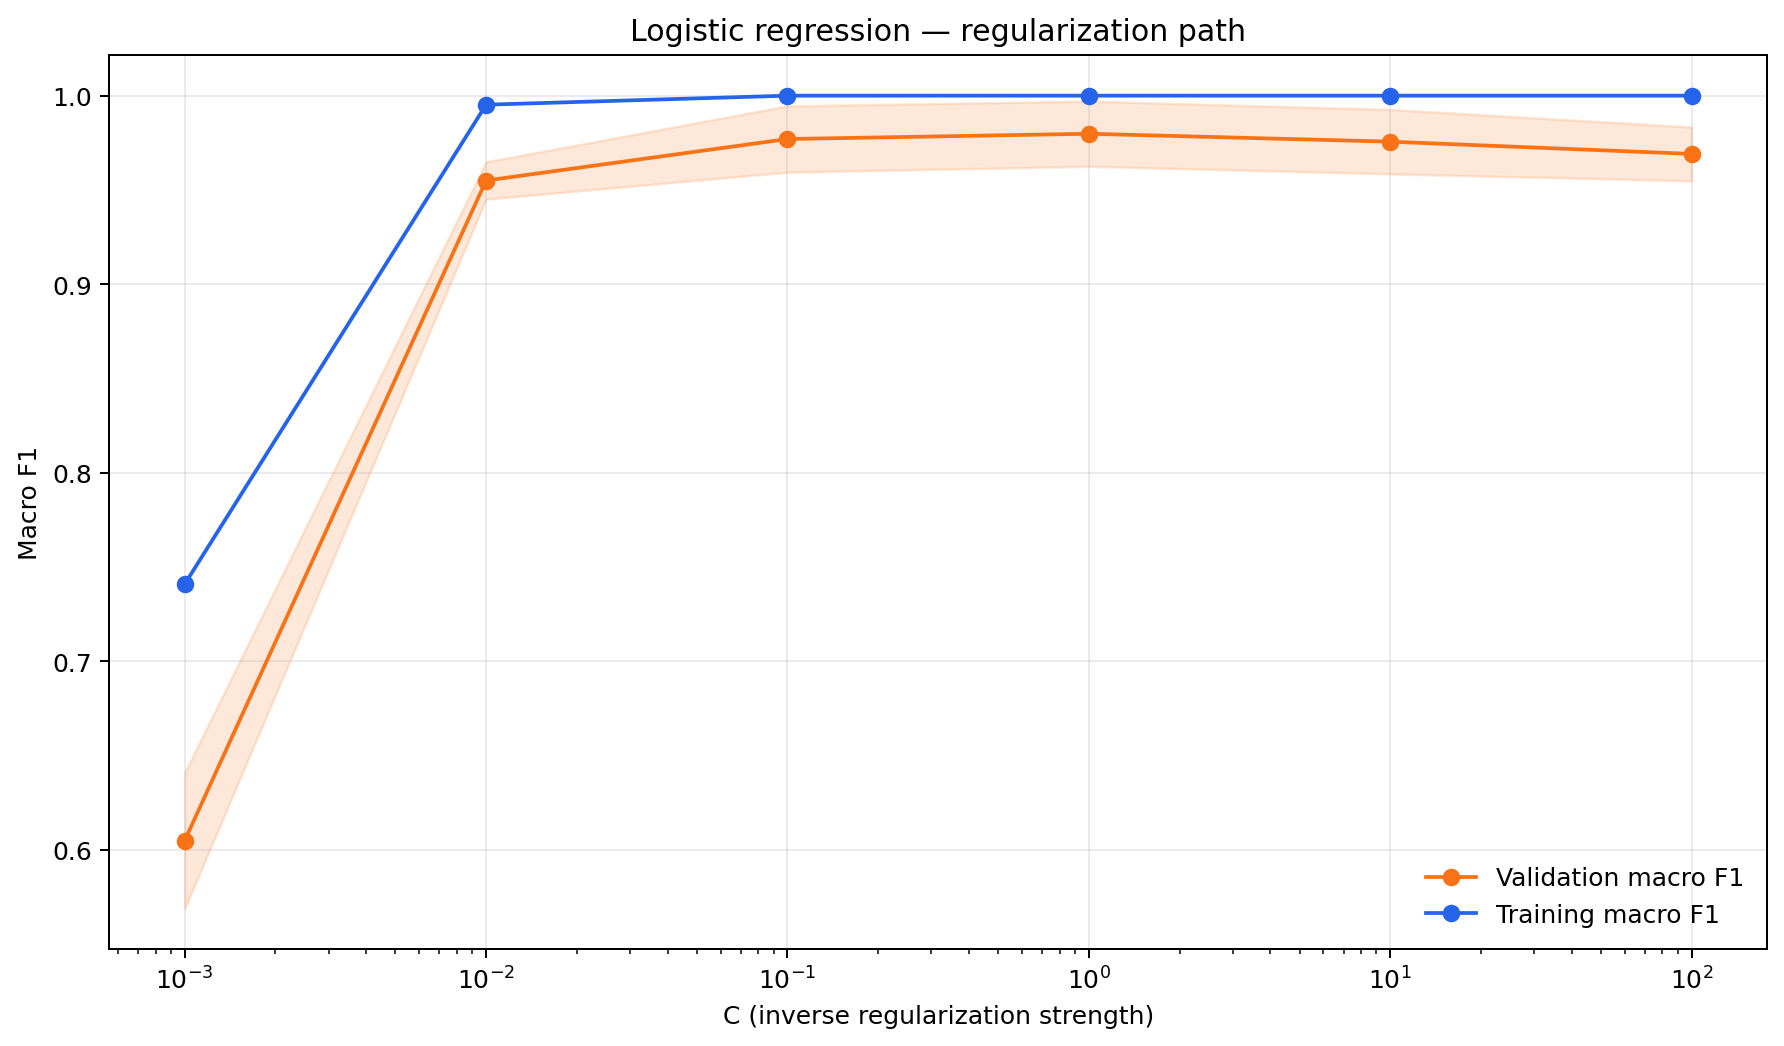
\includegraphics[width=\textwidth]{../figures/en/fig06_regularization_path.png}
\caption{Exploratory diagnostic of the tradeoff between regularization and performance. This figure supports model interpretation without replacing the confirmatory estimate.}
\end{figure}

\begin{figure}[H]
\centering
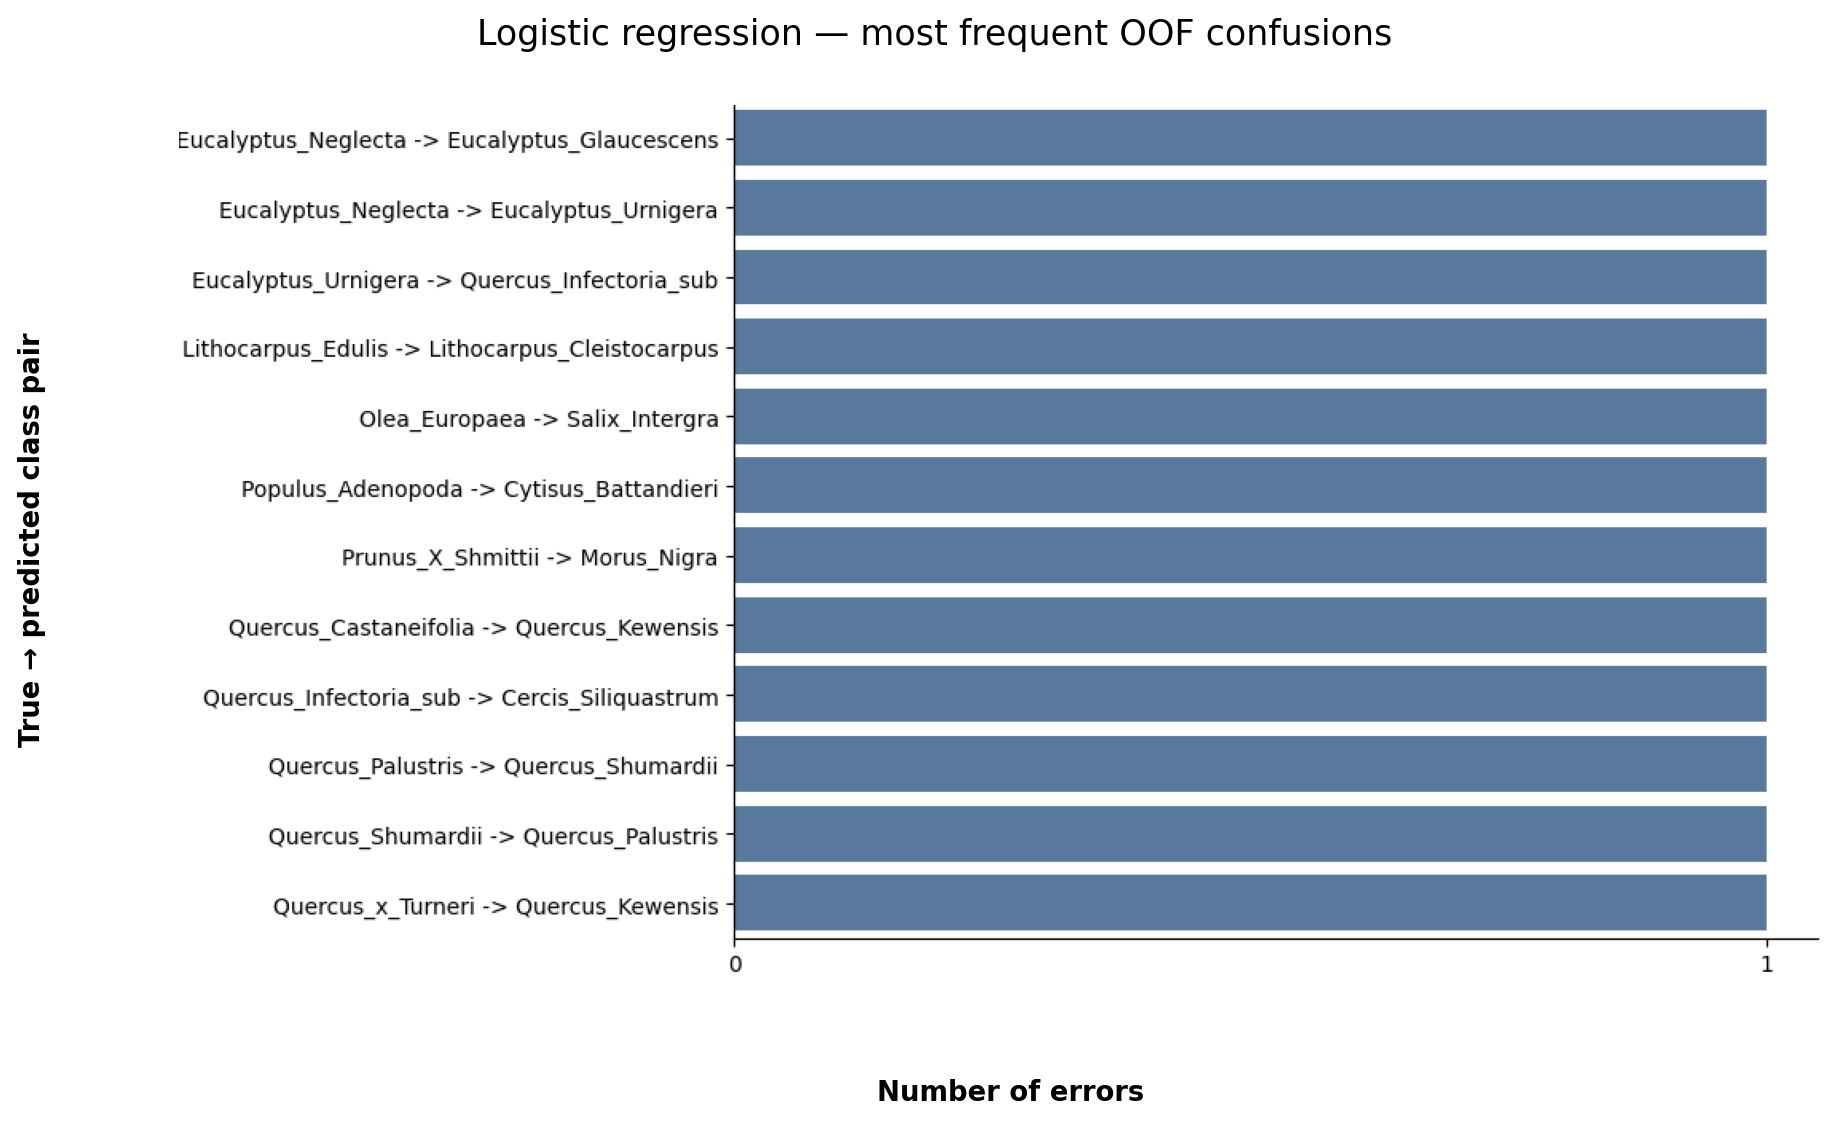
\includegraphics[width=\textwidth]{../figures/en/fig_lr_top12_confusions.png}
\caption{Leading residual confusions for logistic regression. Their small number is consistent with the observed confirmatory performance.}
\end{figure}

\subsubsection{Secondary corroboration}
Secondary corroboration fully supports the primary result. The \texttt{scaled\_only} reference, the \texttt{scaled\_pca} variant, and the \texttt{tuned} variant all achieve \texttt{0.9892} in \texttt{F1-macro} and \texttt{0.9899} in \texttt{accuracy} on the frozen split. The \texttt{tuned - reference} delta is therefore zero.

\begin{table}[H]
\centering
\begin{tabular}{|l|r|r|l|}
\hline
\textbf{Variant} & \textbf{Corroboration F1} & \textbf{Corroboration accuracy} & \textbf{Role} \\
\hline
\texttt{default} & \texttt{0.4800} & \texttt{0.5253} & baseline \\
\texttt{scaled\_only} & \texttt{0.9892} & \texttt{0.9899} & reference \\
\texttt{scaled\_pca} & \texttt{0.9892} & \texttt{0.9899} & descriptive \\
\texttt{tuned} & \texttt{0.9892} & \texttt{0.9899} & tuned \\
\hline
\end{tabular}
\end{table}

For logistic regression, corroboration extends a result already evident in the preceding analyses: after standardization, the family is both highly effective and remarkably stable. This combination, even more than tuning itself, makes it the report's practical reference.

\begin{figure}[H]
\centering
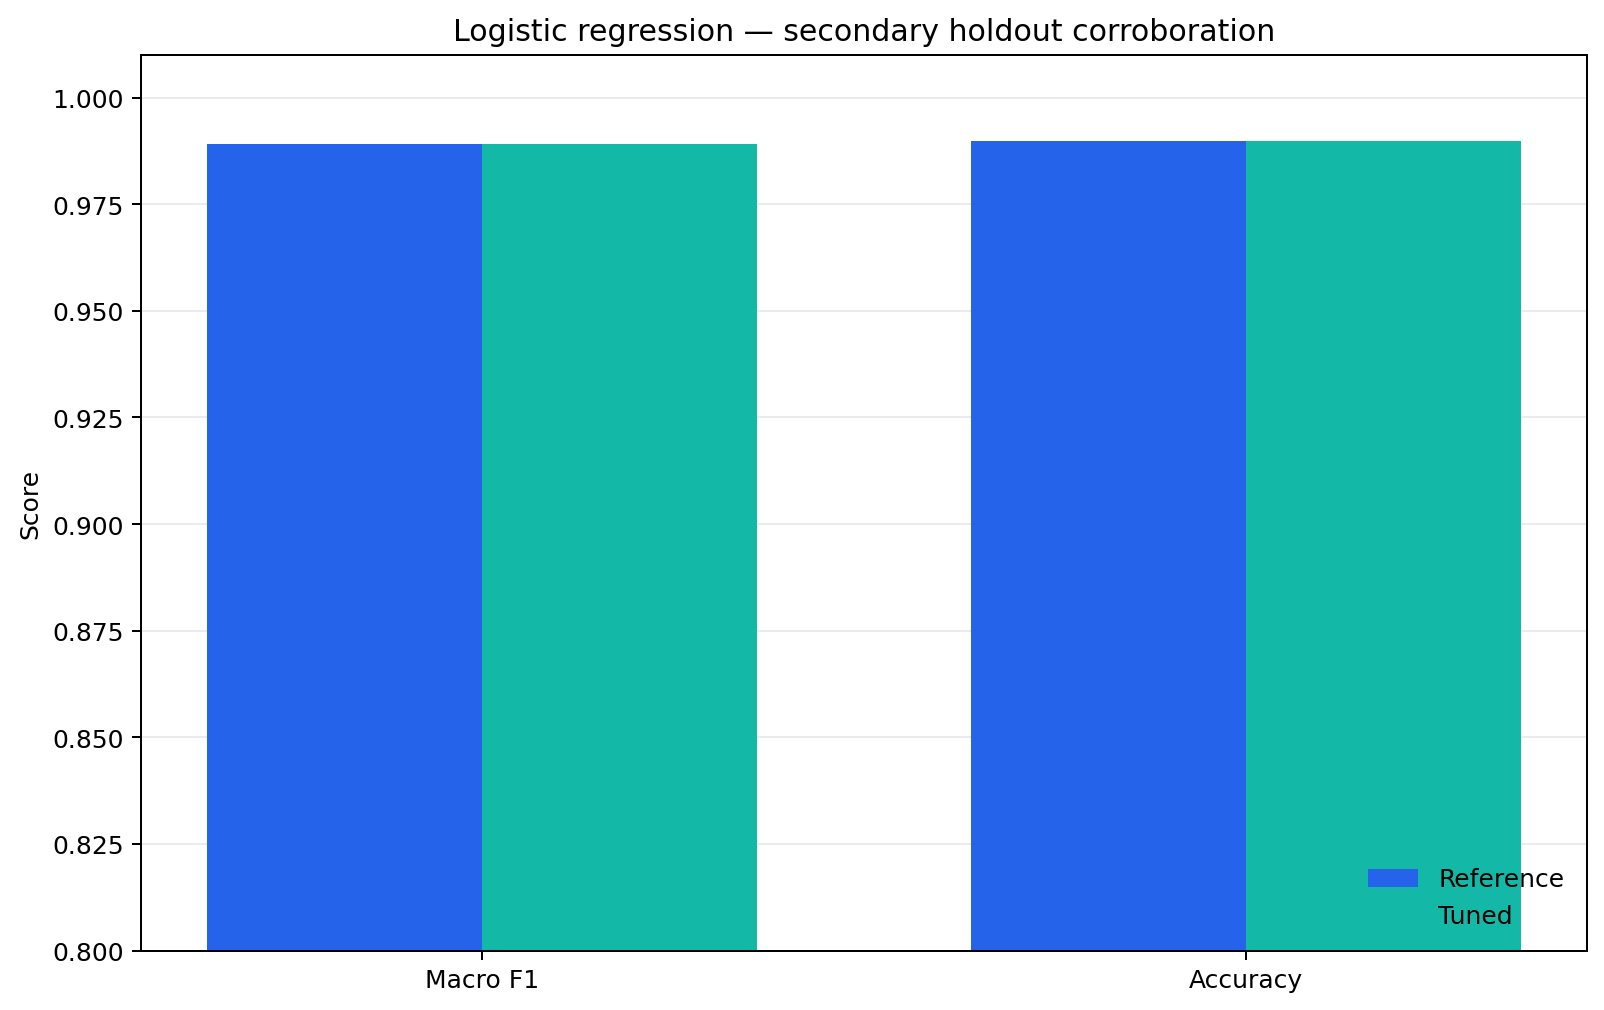
\includegraphics[width=\textwidth]{../figures/en/fig_lr_corroboration_holdout.png}
\caption{Secondary comparison between the reference and \texttt{tuned} logistic-regression variants on the corroboration set.}
\end{figure}

% --- SVM ---
\subsection{RBF SVM model}

\subsubsection{Role of the model}
The RBF-kernel SVM is the reference nonlinear margin-based method. Its purpose is to determine whether a more flexible boundary than that of the linear models can provide a tangible gain while remaining controlled on a moderately sized dataset.

\subsubsection{Exploration}
The SVM is already strong without preprocessing, with a \texttt{F1-macro} of \texttt{0.8389} and an \texttt{accuracy} of \texttt{0.8561}. Standardization nevertheless produces a clear change in scale: both \texttt{scaled\_only} and \texttt{scaled\_pca} reach \texttt{0.9712} in \texttt{F1-macro} and \texttt{0.9785} in \texttt{accuracy}. \texttt{PCA} therefore does not change the empirical interpretation, whereas scaling appears to be the decisive condition for using the RBF kernel effectively.

\begin{table}[H]
\centering
\begin{tabular}{|l|l|r|r|r|r|}
\hline
\textbf{Variant} & \textbf{Protocol} & \textbf{Macro F1} & \textbf{Accuracy} & \textbf{F1 gap} & \textbf{Time (s)} \\
\hline
\texttt{default} & simple CV & \texttt{0.8389} & \texttt{0.8561} & \texttt{0.1364} & \texttt{2.36} \\
\texttt{scaled\_only} & simple CV & \texttt{0.9712} & \texttt{0.9785} & \texttt{0.0266} & \texttt{2.45} \\
\texttt{scaled\_pca} & simple CV & \texttt{0.9712} & \texttt{0.9785} & \texttt{0.0266} & \texttt{2.50} \\
\hline
\end{tabular}
\end{table}

The SVM therefore joins the leading group during the exploratory stage. It combines very strong performance with a limited generalization gap, fully justifying its inclusion among the study's central models.

\begin{figure}[H]
\centering
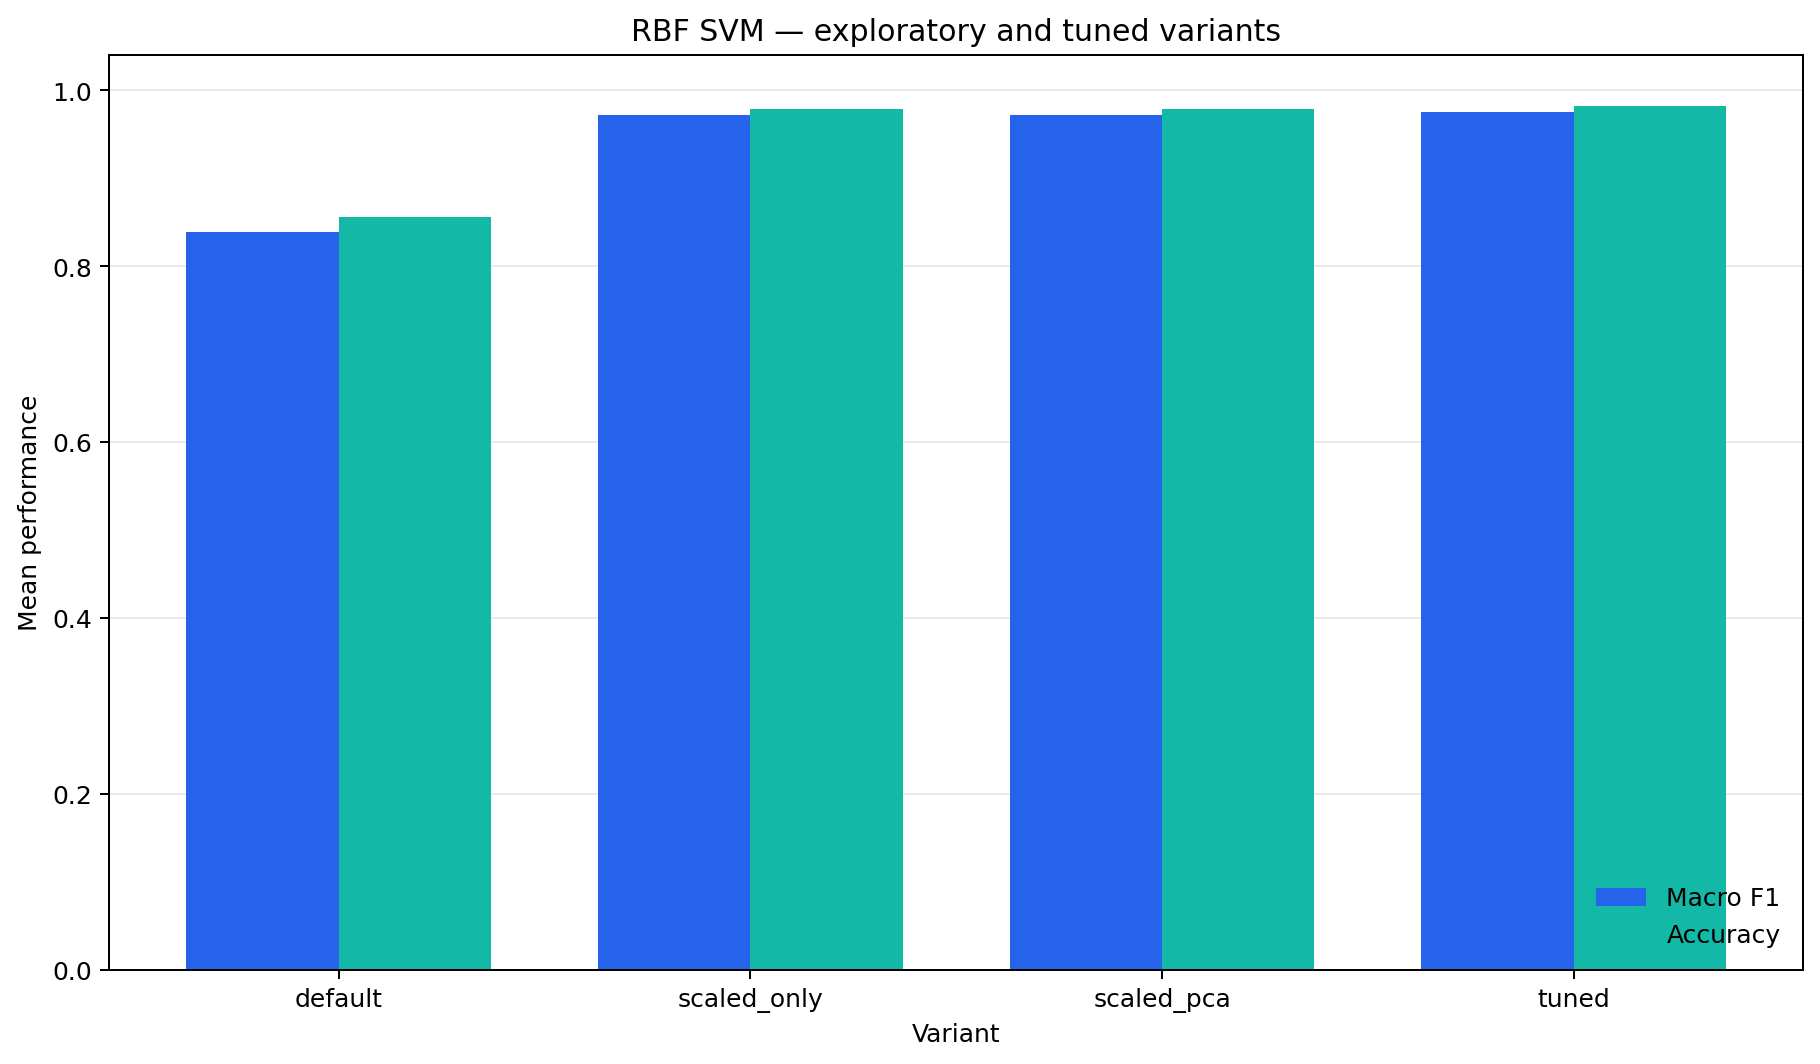
\includegraphics[width=\textwidth]{../figures/en/fig_svm_comparaison_variantes.png}
\caption{Exploratory comparison of SVM variants. The RBF kernel becomes fully competitive after feature standardization.}
\end{figure}

\subsubsection{Confirmation}
Nested cross-validation confirms this leading position. The \texttt{tuned} variant achieves a mean \texttt{F1-macro} of \texttt{0.9756} and mean \texttt{accuracy} of \texttt{0.9823}, with standard deviations of \texttt{0.0207} and \texttt{0.0151}. The confirmatory score is slightly higher than those of the best exploratory variants, suggesting that tuning is useful but moderate.

\begin{table}[H]
\centering
\begin{tabular}{|l|r|}
\hline
\textbf{Confirmatory metric} & \textbf{Value} \\
\hline
Mean Macro F1 & \texttt{0.9756} \\
F1 standard deviation & \texttt{0.0207} \\
Mean accuracy & \texttt{0.9823} \\
Accuracy standard deviation & \texttt{0.0151} \\
Protocol & \texttt{nested CV} \\
Outer folds & \texttt{5} \\
Inner folds & \texttt{3} \\
Total time (s) & \texttt{56.49} \\
\hline
\end{tabular}
\end{table}

The SVM also belongs to the leading confirmatory pair, with a mean very close to that of logistic regression. It therefore provides an excellent nonlinear alternative, at the cost of higher training time and lower structural interpretability.

\subsubsection{Descriptive diagnostics}
\begin{sloppypar}
The exploratory tuning table shows that the best performance is concentrated in a compact region of the hyperparameter space. Two findings dominate. Setting \texttt{gamma = 0.1} sharply degrades the scores. In addition, \texttt{PCA} provides no robust gain over the standardized pipeline without dimensionality reduction. The best exploratory setting is therefore \texttt{C = 10} with \texttt{gamma = scale}, without \texttt{PCA}.
\end{sloppypar}

\begin{table}[H]
\centering
\begin{tabular}{|l|r|r|r|}
\hline
\textbf{C / gamma} & \textbf{scale} & \textbf{0.01} & \textbf{0.1} \\
\hline
\texttt{1} & \texttt{0.9697} & \texttt{0.9693} & \texttt{0.2539} \\
\texttt{10} & \texttt{0.9700} & \texttt{0.9679} & \texttt{0.2885} \\
\hline
\end{tabular}
\caption{Exploratory SVM tuning without PCA (mean CV \texttt{F1-macro})}
\end{table}

\begin{table}[H]
\centering
\begin{tabular}{|l|r|r|r|}
\hline
\textbf{C / gamma} & \textbf{scale} & \textbf{0.01} & \textbf{0.1} \\
\hline
\texttt{1} & \texttt{0.9697} & \texttt{0.9679} & \texttt{0.2917} \\
\texttt{10} & \texttt{0.9688} & \texttt{0.9654} & \texttt{0.3402} \\
\hline
\end{tabular}
\caption{Exploratory SVM tuning with PCA (mean CV \texttt{F1-macro})}
\end{table}

Residual confusions remain rare and localized, which is consistent with the quality of the confirmatory score.

\begin{figure}[H]
\centering
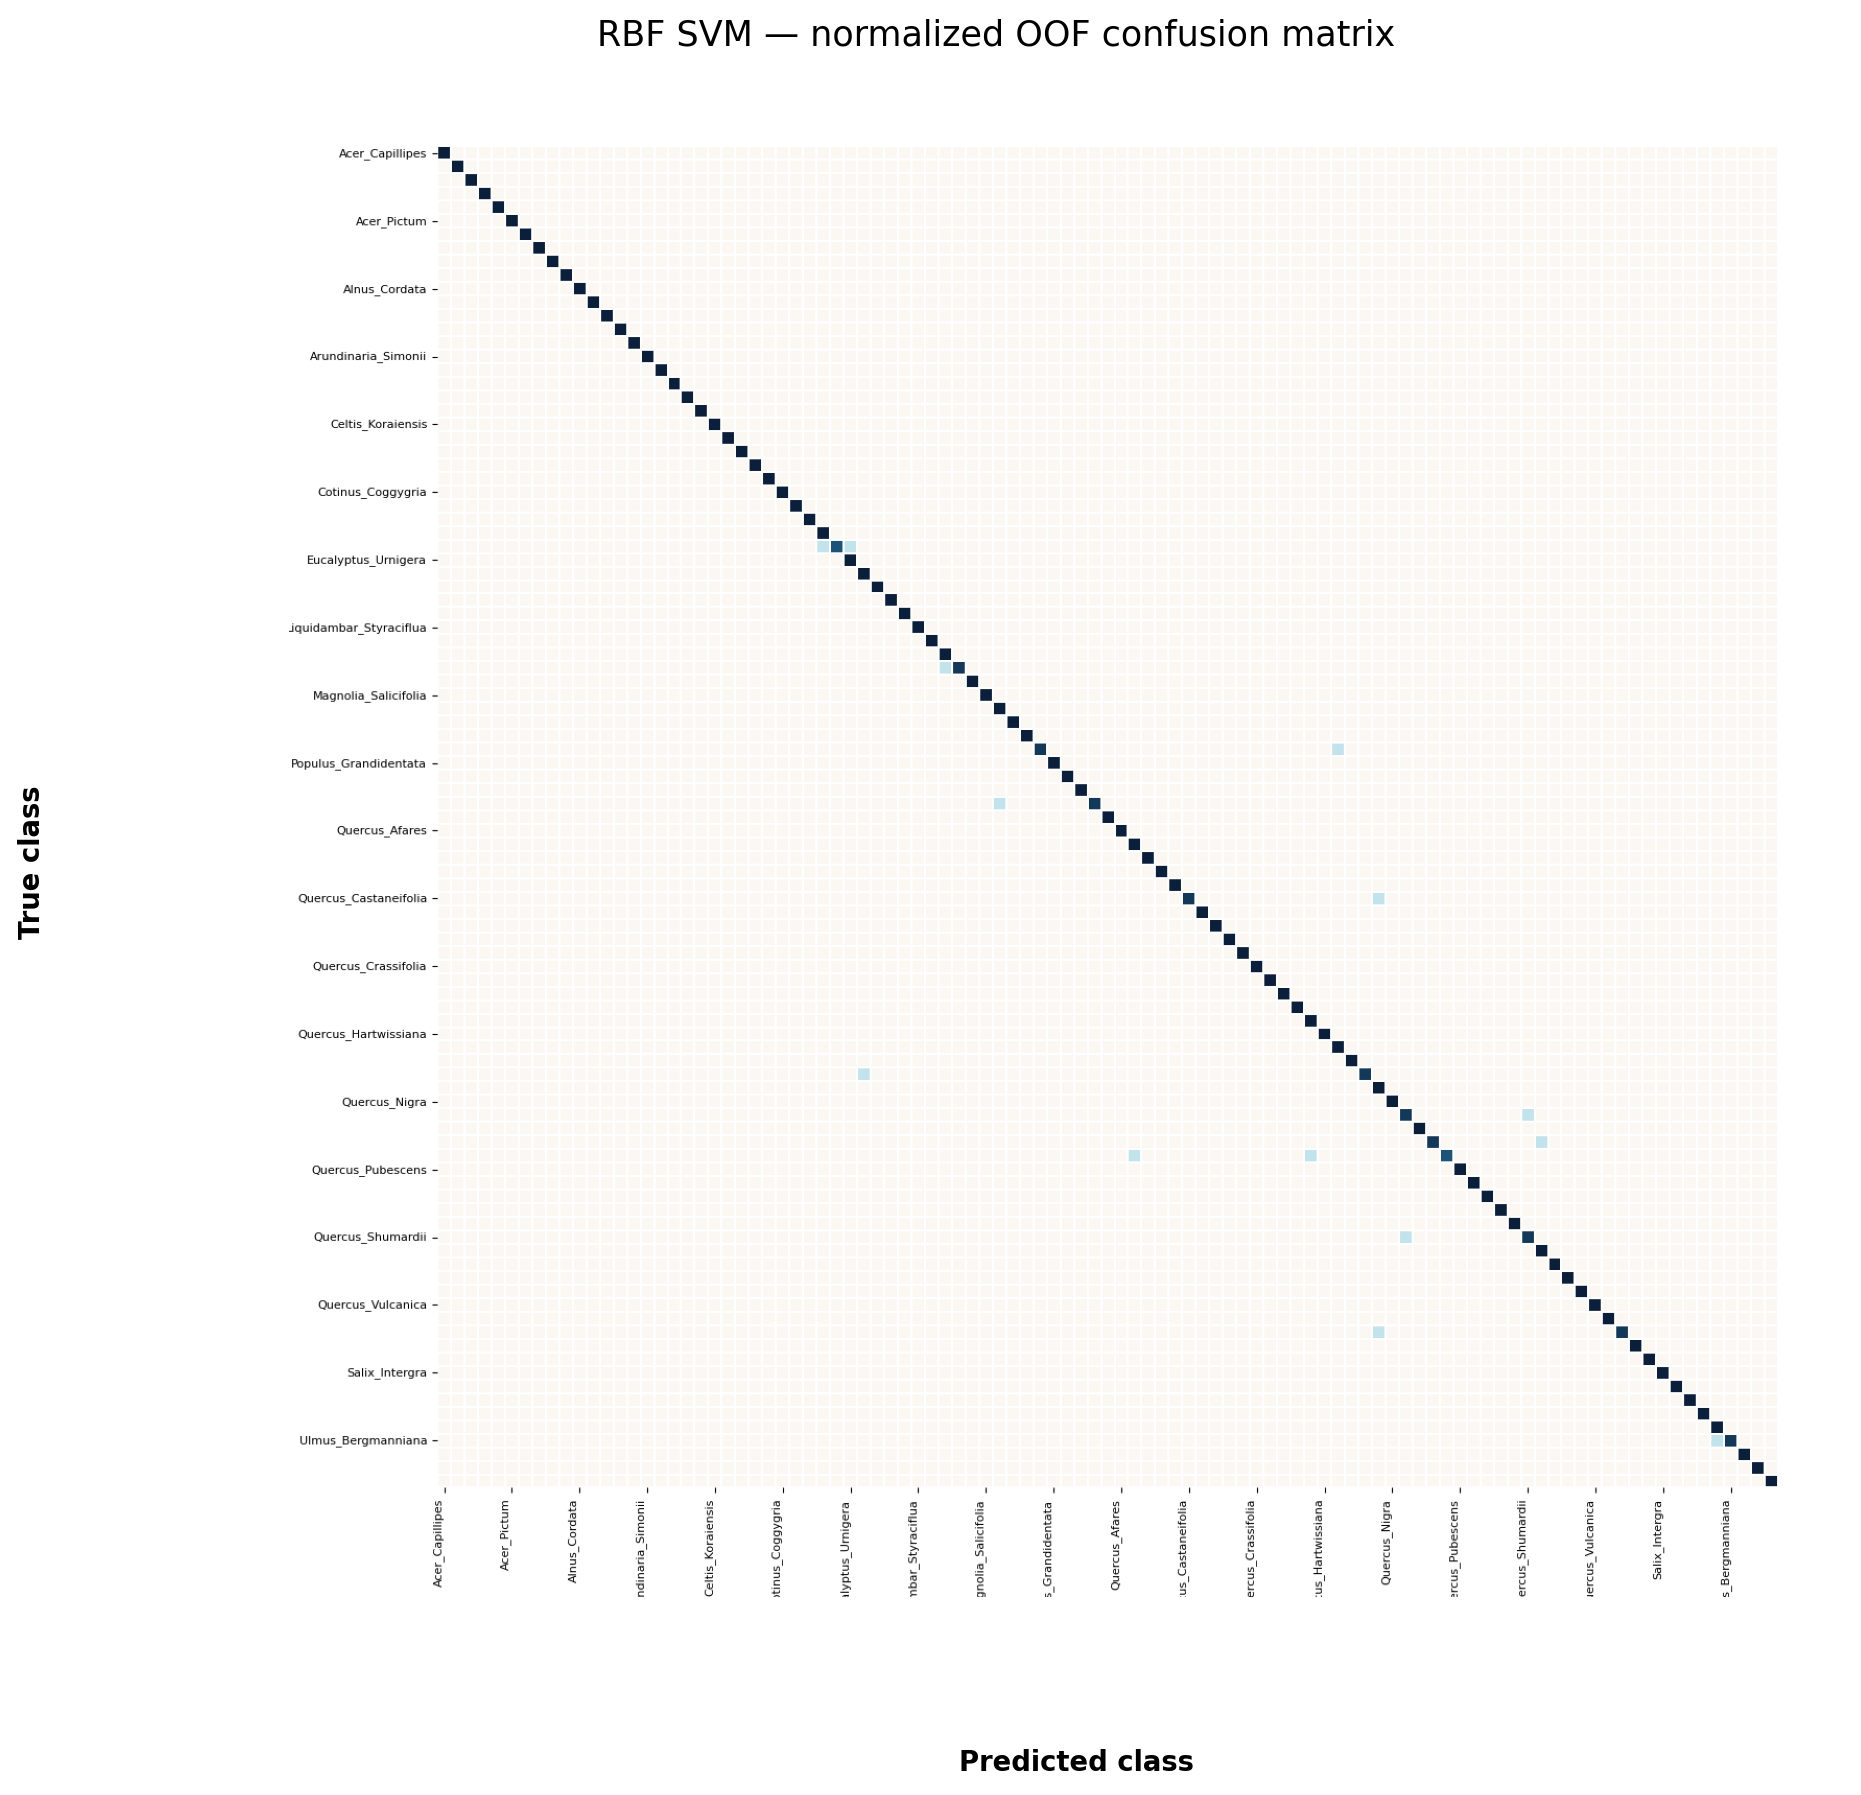
\includegraphics[width=\textwidth]{../figures/en/figA_confusion_svm_tuned.png}
\caption{Normalized confusion matrix from the out-of-fold predictions of the \texttt{tuned} variant. Residual errors are few and concentrated.}
\end{figure}

\begin{figure}[H]
\centering
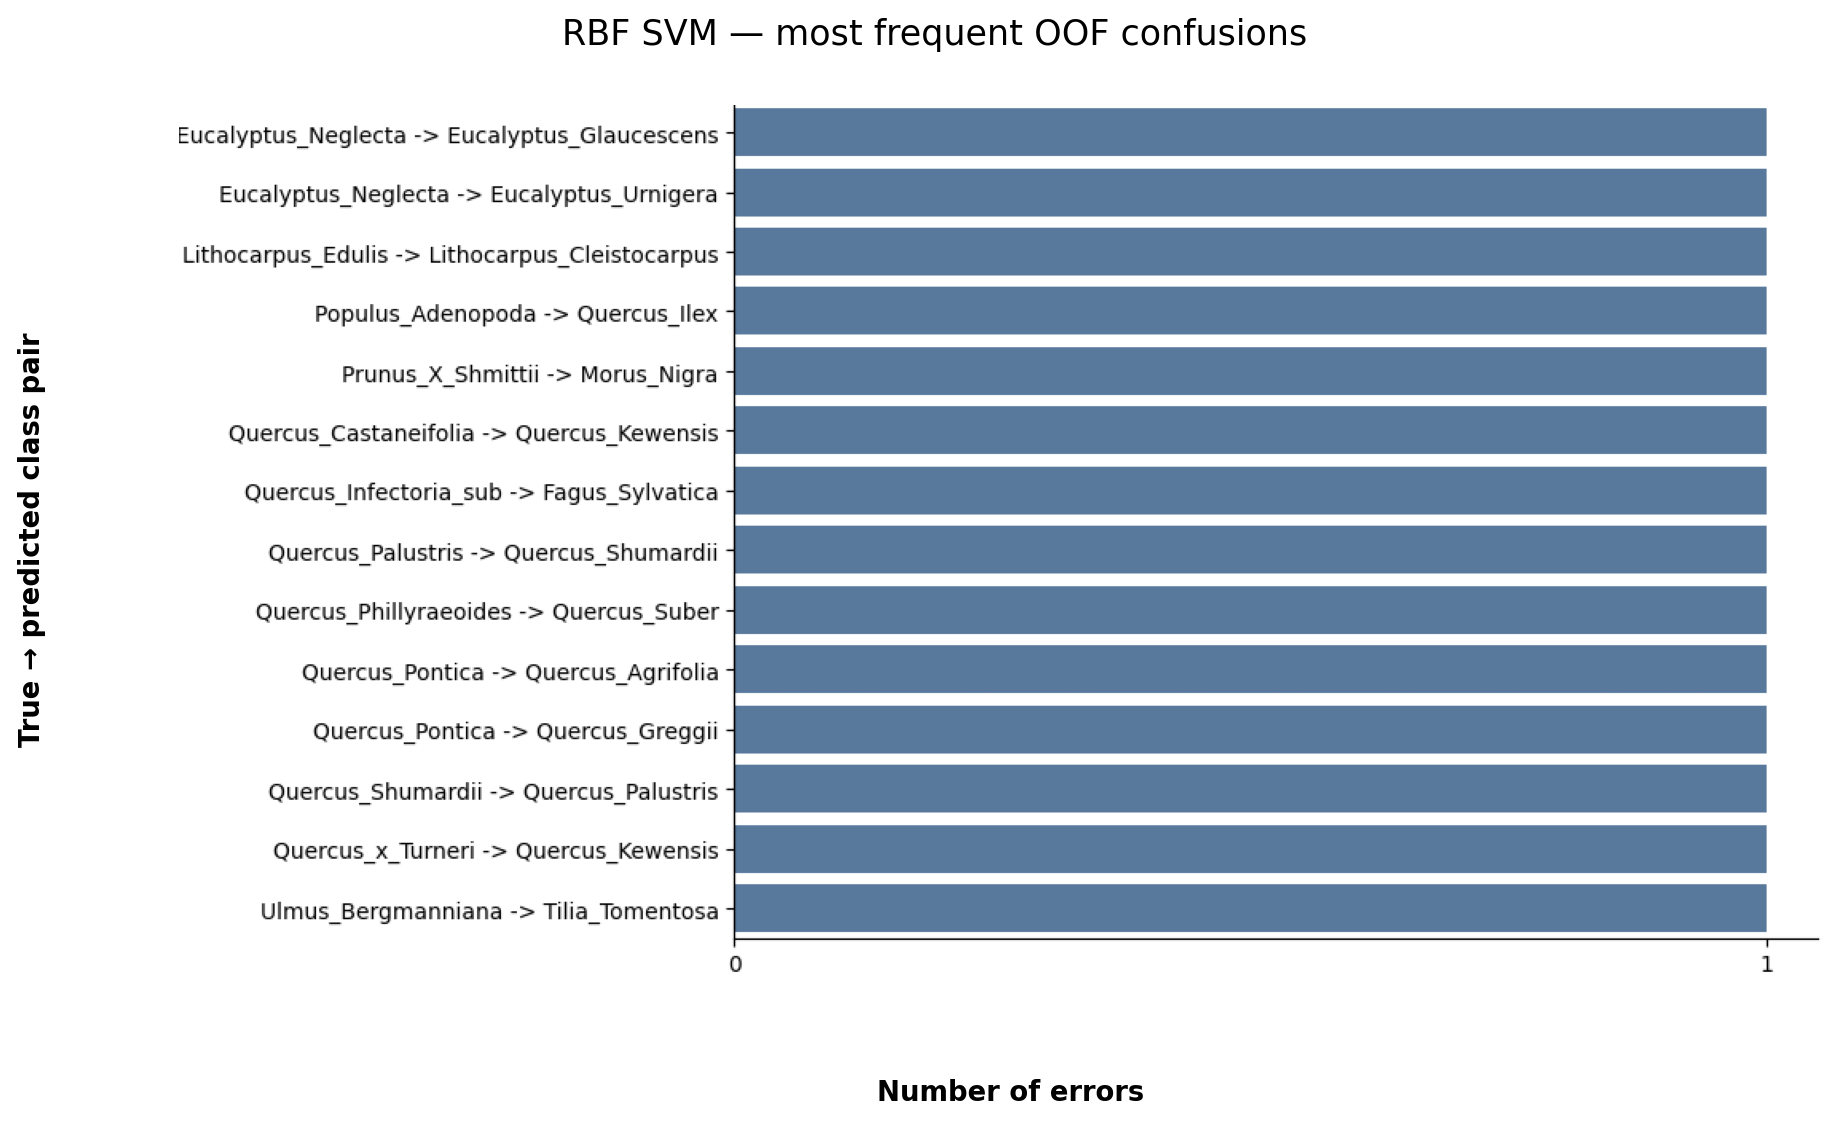
\includegraphics[width=\textwidth]{../figures/en/fig_svm_top12_confusions.png}
\caption{Leading confusions for the tuned SVM. Their limited number indicates that errors are concentrated among a few structurally difficult cases.}
\end{figure}

\subsubsection{Secondary corroboration}
Secondary corroboration is consistent with the confirmatory analysis and provides an even more favorable signal for tuning. The \texttt{scaled\_only} reference achieves \texttt{0.9838} in \texttt{F1-macro} and \texttt{0.9848} in \texttt{accuracy}, while the \texttt{tuned} variant reaches \texttt{0.9946} and \texttt{0.9949}. The \texttt{tuned - reference} delta is therefore \texttt{+0.0108}.

\begin{table}[H]
\centering
\begin{tabular}{|l|r|r|l|}
\hline
\textbf{Variant} & \textbf{Corroboration F1} & \textbf{Corroboration accuracy} & \textbf{Role} \\
\hline
\texttt{default} & \texttt{0.9242} & \texttt{0.9343} & baseline \\
\texttt{scaled\_only} & \texttt{0.9838} & \texttt{0.9848} & reference \\
\texttt{scaled\_pca} & \texttt{0.9838} & \texttt{0.9848} & descriptive \\
\texttt{tuned} & \texttt{0.9946} & \texttt{0.9949} & tuned \\
\hline
\end{tabular}
\end{table}

For the SVM, corroboration retains clear practical value: tuning remains beneficial on the frozen split. The family therefore emerges as one of the report's most compelling solutions, very close to logistic regression in performance but more dependent on careful hyperparameter selection.

\begin{figure}[H]
\centering
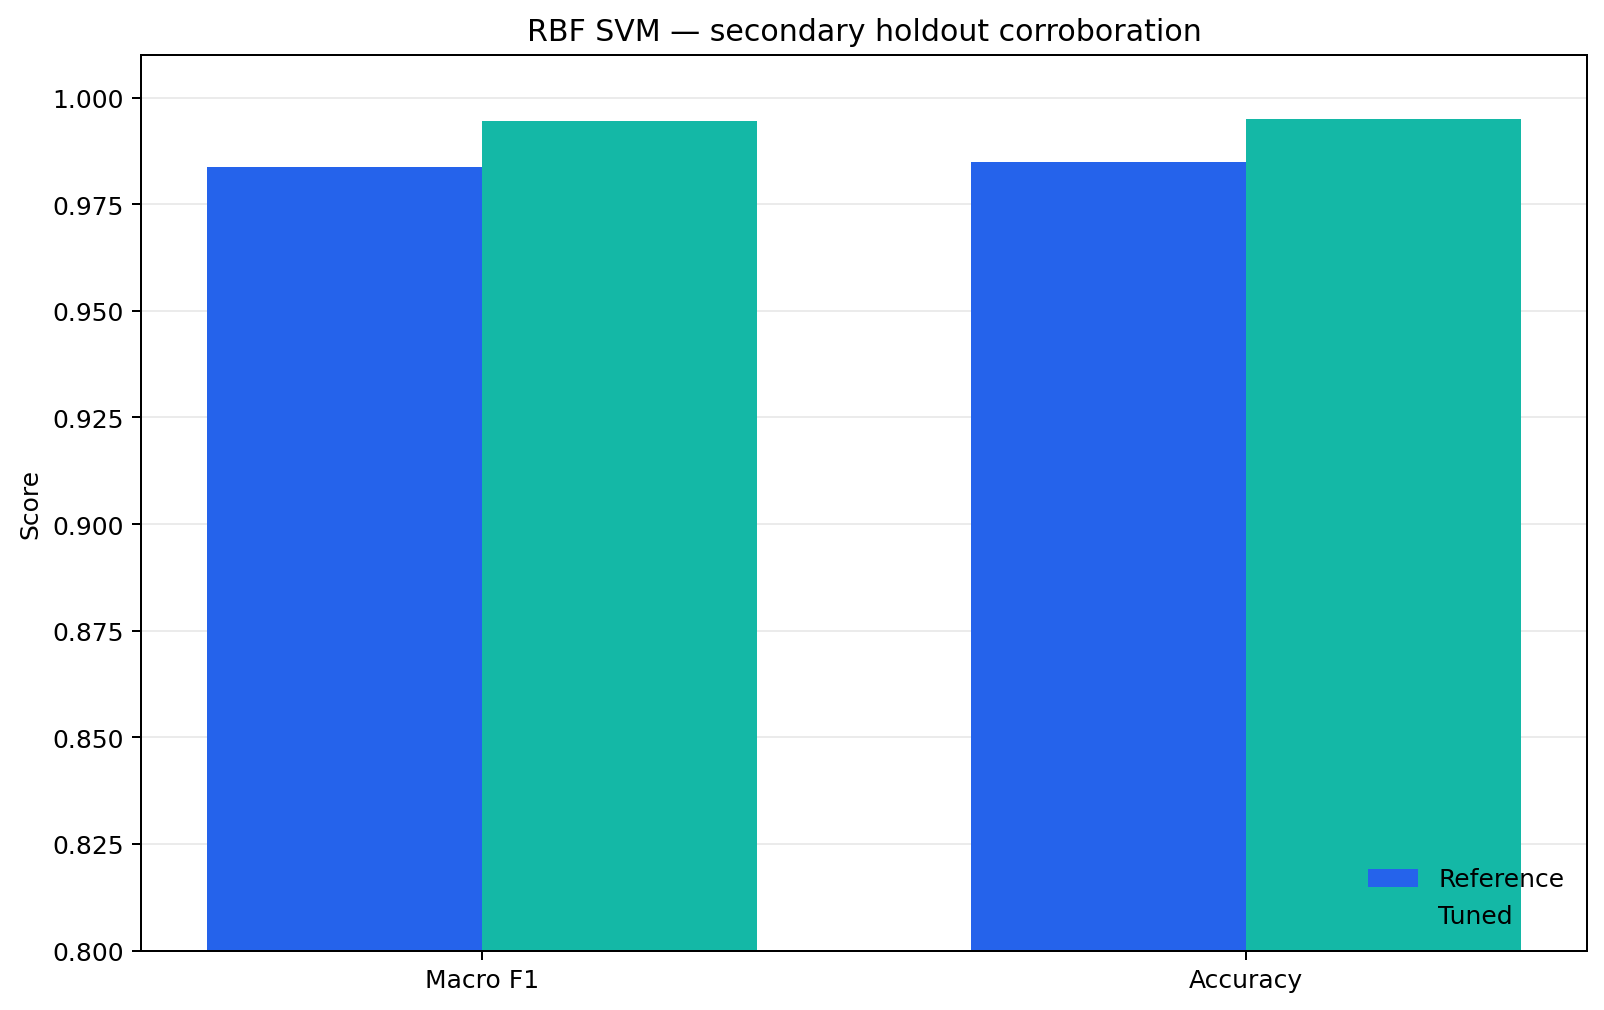
\includegraphics[width=\textwidth]{../figures/en/fig_svm_corroboration_holdout.png}
\caption{Secondary comparison between the reference and \texttt{tuned} SVM variants on the corroboration set.}
\end{figure}

% --- RANDOM FOREST ---
\subsection{Random forest model}

\subsubsection{Role of the model}
The random forest represents the study's tree-ensemble family. It is particularly relevant here because it can capture nonlinear interactions without requiring feature scaling and because it stabilizes the splits that a single decision tree struggles to generalize.

\subsubsection{Exploration}
The exploratory evidence is highly favorable for this family. The \texttt{default} variant achieves \texttt{0.9764} in \texttt{F1-macro} and \texttt{0.9785} in \texttt{accuracy}, with a contained generalization gap (\texttt{0.0236}). The \texttt{restricted\_depth} variant, added as a complexity control, falls to \texttt{0.9345} in \texttt{F1-macro} and \texttt{0.9445} in \texttt{accuracy}. Restricting depth therefore slightly reduces computation time but markedly degrades performance.

\begin{table}[H]
\centering
\begin{tabular}{|l|l|r|r|r|r|}
\hline
\textbf{Variant} & \textbf{Protocol} & \textbf{Macro F1} & \textbf{Accuracy} & \textbf{F1 gap} & \textbf{Time (s)} \\
\hline
\texttt{default} & simple CV & \texttt{0.9764} & \texttt{0.9785} & \texttt{0.0236} & \texttt{9.16} \\
\texttt{restricted\_depth} & simple CV & \texttt{0.9345} & \texttt{0.9445} & \texttt{0.0651} & \texttt{5.42} \\
\hline
\end{tabular}
\end{table}

Even at this stage, the random forest ranks among the project's best models. Its main strength is achieving this level without sophisticated preprocessing, making it a robust and straightforward option for already informative tabular variables.

\begin{figure}[H]
\centering
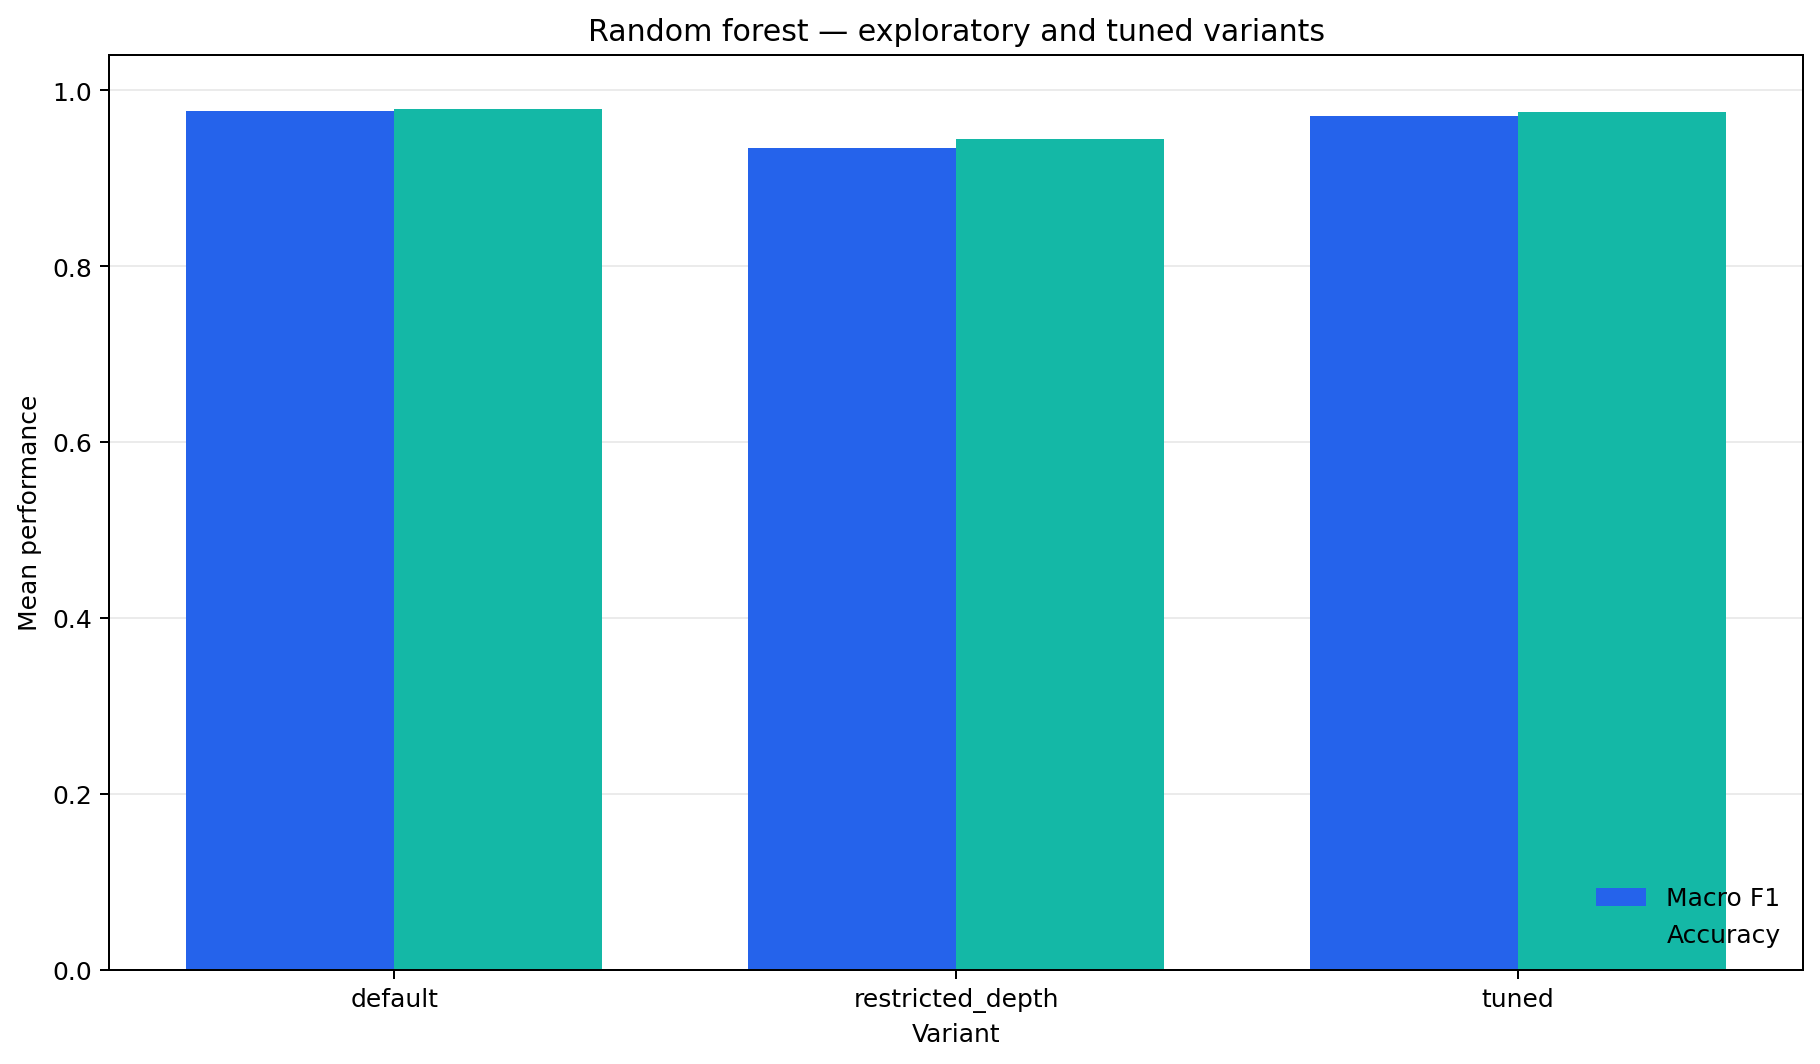
\includegraphics[width=\textwidth]{../figures/en/fig_rf_comparaison_variantes.png}
\caption{Exploratory comparison of random-forest variants. The default version already performs extremely well, and restricting depth proves too costly in performance.}
\end{figure}

\subsubsection{Confirmation}
Nested cross-validation yields a mean \texttt{F1-macro} of \texttt{0.9702} and mean \texttt{accuracy} of \texttt{0.9747}, with standard deviations of \texttt{0.0140} and \texttt{0.0089}. The confirmatory score remains slightly below that of the best exploratory variant, as expected when the estimate corrects for selection optimism.

\begin{table}[H]
\centering
\begin{tabular}{|l|r|}
\hline
\textbf{Confirmatory metric} & \textbf{Value} \\
\hline
Mean Macro F1 & \texttt{0.9702} \\
F1 standard deviation & \texttt{0.0140} \\
Mean accuracy & \texttt{0.9747} \\
Accuracy standard deviation & \texttt{0.0089} \\
Protocol & \texttt{nested CV} \\
Outer folds & \texttt{5} \\
Inner folds & \texttt{3} \\
Total time (s) & \texttt{250.11} \\
\hline
\end{tabular}
\end{table}

The random forest thus remains among the top three. It ranks slightly behind logistic regression and the SVM, but is still highly competitive and remarkably stable. Its main cost is a longer training time than the linear models.

\subsubsection{Descriptive diagnostics}
The \texttt{OOB} curve shows that marginal gains stabilize quickly as the number of trees increases. This pattern is fully consistent with the strong performance of the \texttt{default} variant and with tuning that is progressive rather than disruptive. The confusion figures further confirm that residual errors remain rare and structured.

\begin{figure}[H]
\centering
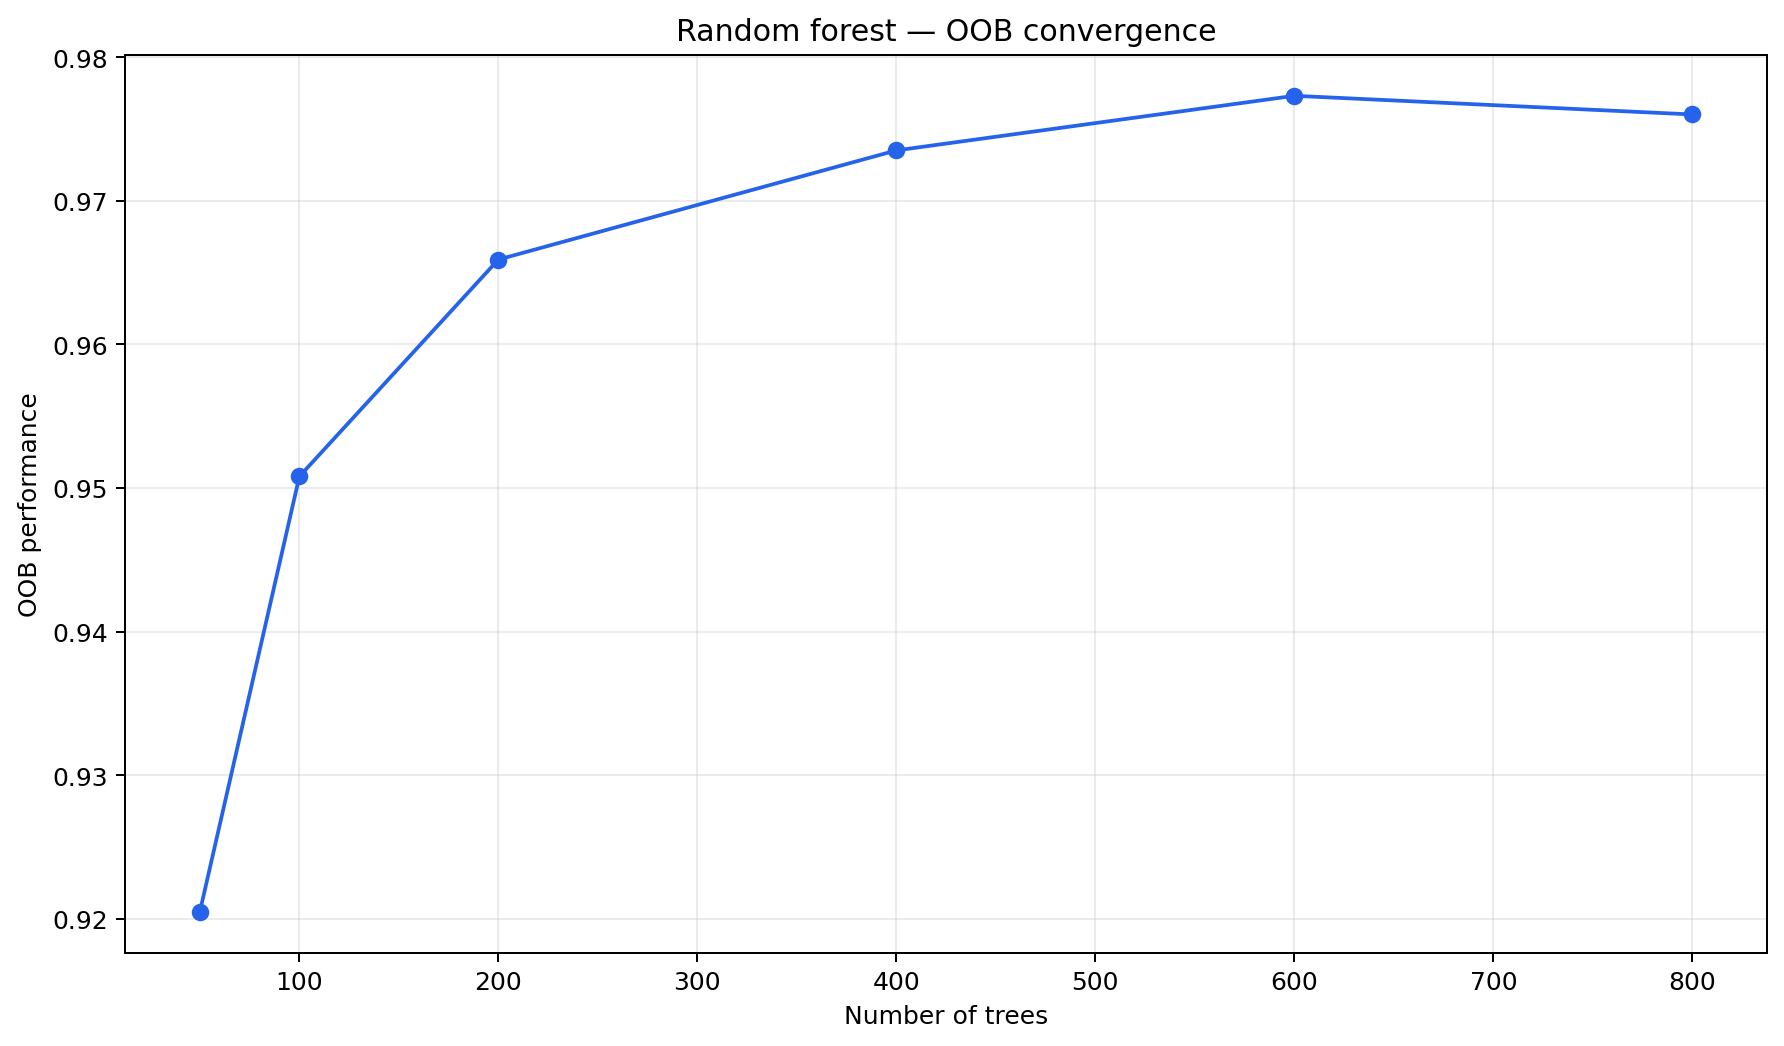
\includegraphics[width=\textwidth]{../figures/en/fig10_oob_vs_n_estimators.png}
\caption{Exploratory evolution of the OOB score with the number of trees. The curve suggests that performance stabilizes quickly once the forest is sufficiently large.}
\end{figure}

\begin{figure}[H]
\centering
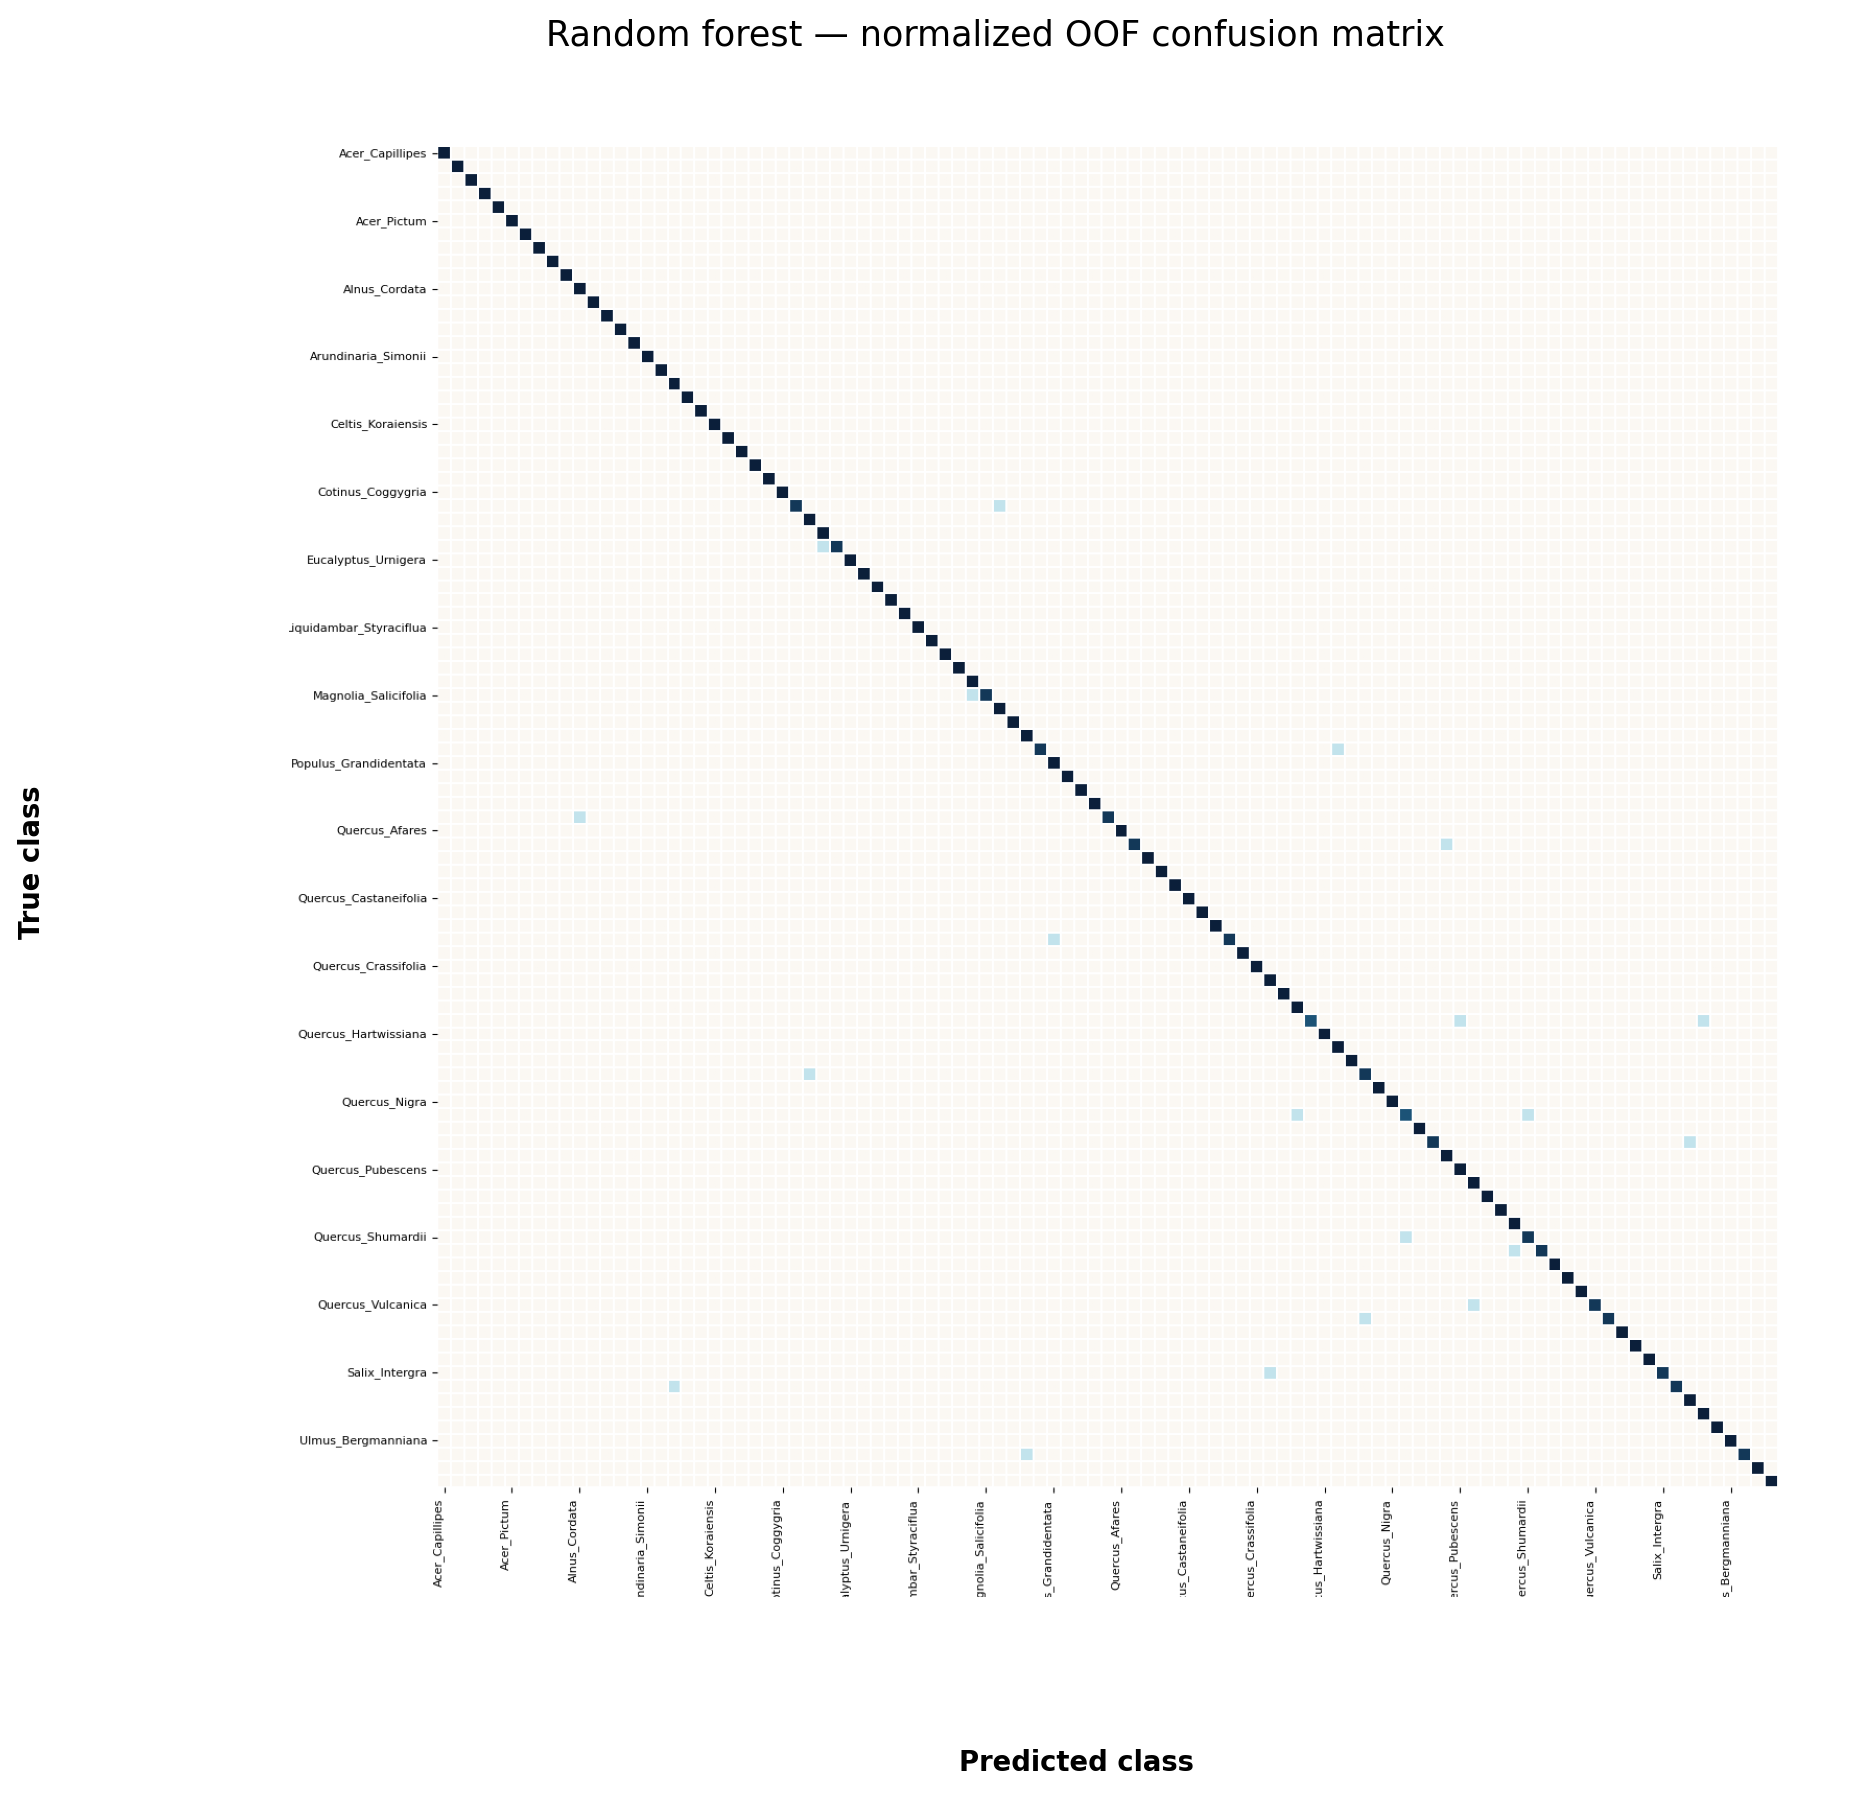
\includegraphics[width=\textwidth]{../figures/en/figA_confusion_rf_tuned.png}
\caption{Normalized confusion matrix obtained from the out-of-fold predictions of the \texttt{tuned} variant. The pattern remains very close to that of the project's best models.}
\end{figure}

\begin{figure}[H]
\centering
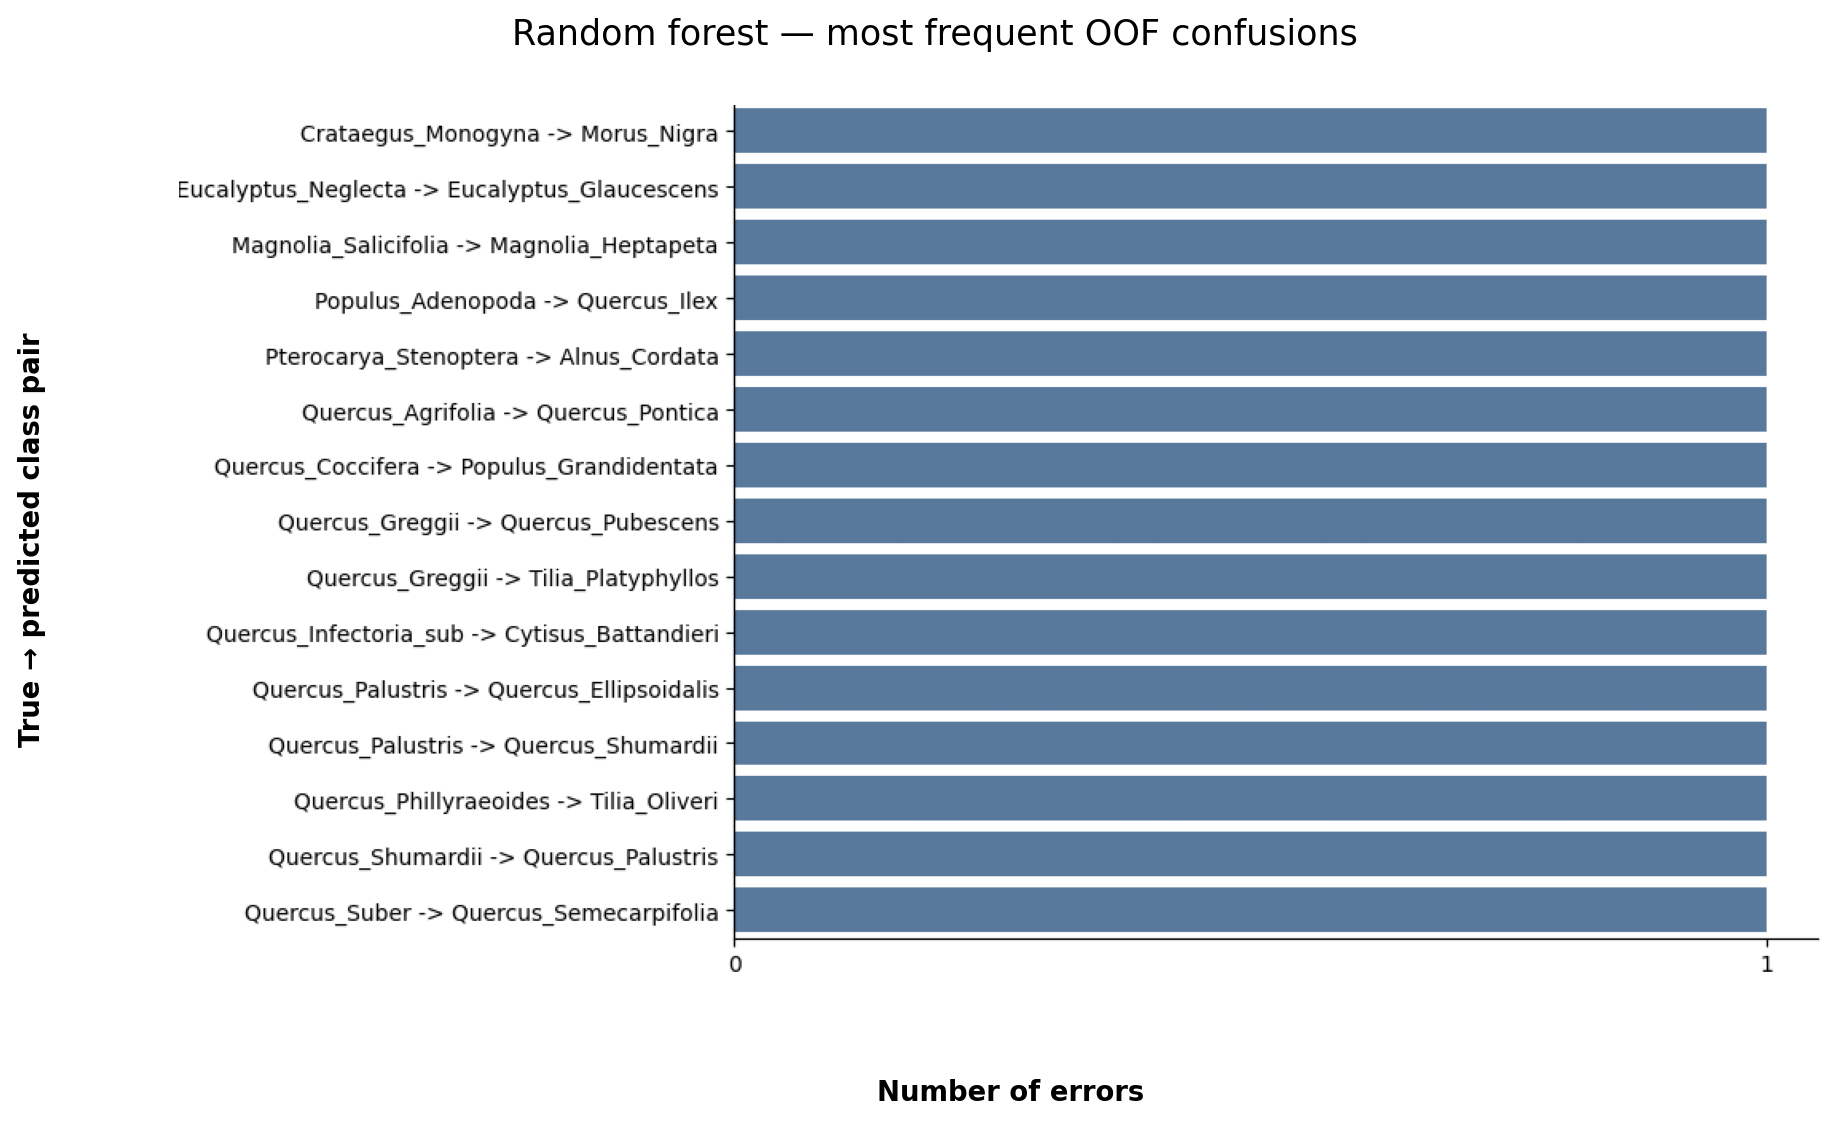
\includegraphics[width=\textwidth]{../figures/en/fig_rf_top12_confusions.png}
\caption{Leading residual confusions for the random forest. Their limited number confirms the problem's strong effective separability for this family.}
\end{figure}

\subsubsection{Secondary corroboration}
Secondary corroboration is available on the frozen split. The selected reference is the \texttt{default} variant, chosen from the exploratory results on the development set. On the corroboration set, \texttt{default} and \texttt{tuned} obtain exactly the same scores: \texttt{0.9842} in \texttt{F1-macro} and \texttt{0.9848} in \texttt{accuracy}. The \texttt{tuned - reference} delta is therefore zero.

\begin{table}[H]
\centering
\begin{tabular}{|l|r|r|l|}
\hline
\textbf{Variant} & \textbf{Corroboration F1} & \textbf{Corroboration accuracy} & \textbf{Role} \\
\hline
\texttt{default} & \texttt{0.9842} & \texttt{0.9848} & reference \\
\texttt{restricted\_depth} & \texttt{0.9468} & \texttt{0.9545} & descriptive \\
\texttt{tuned} & \texttt{0.9842} & \texttt{0.9848} & tuned \\
\hline
\end{tabular}
\end{table}

Here, corroboration confirms the family's excellent performance without providing clear evidence of an additional gain from tuning. The random forest therefore remains a leading, robust, and highly effective model, although its default configuration is already close to the practical optimum on this dataset.

\begin{figure}[H]
\centering
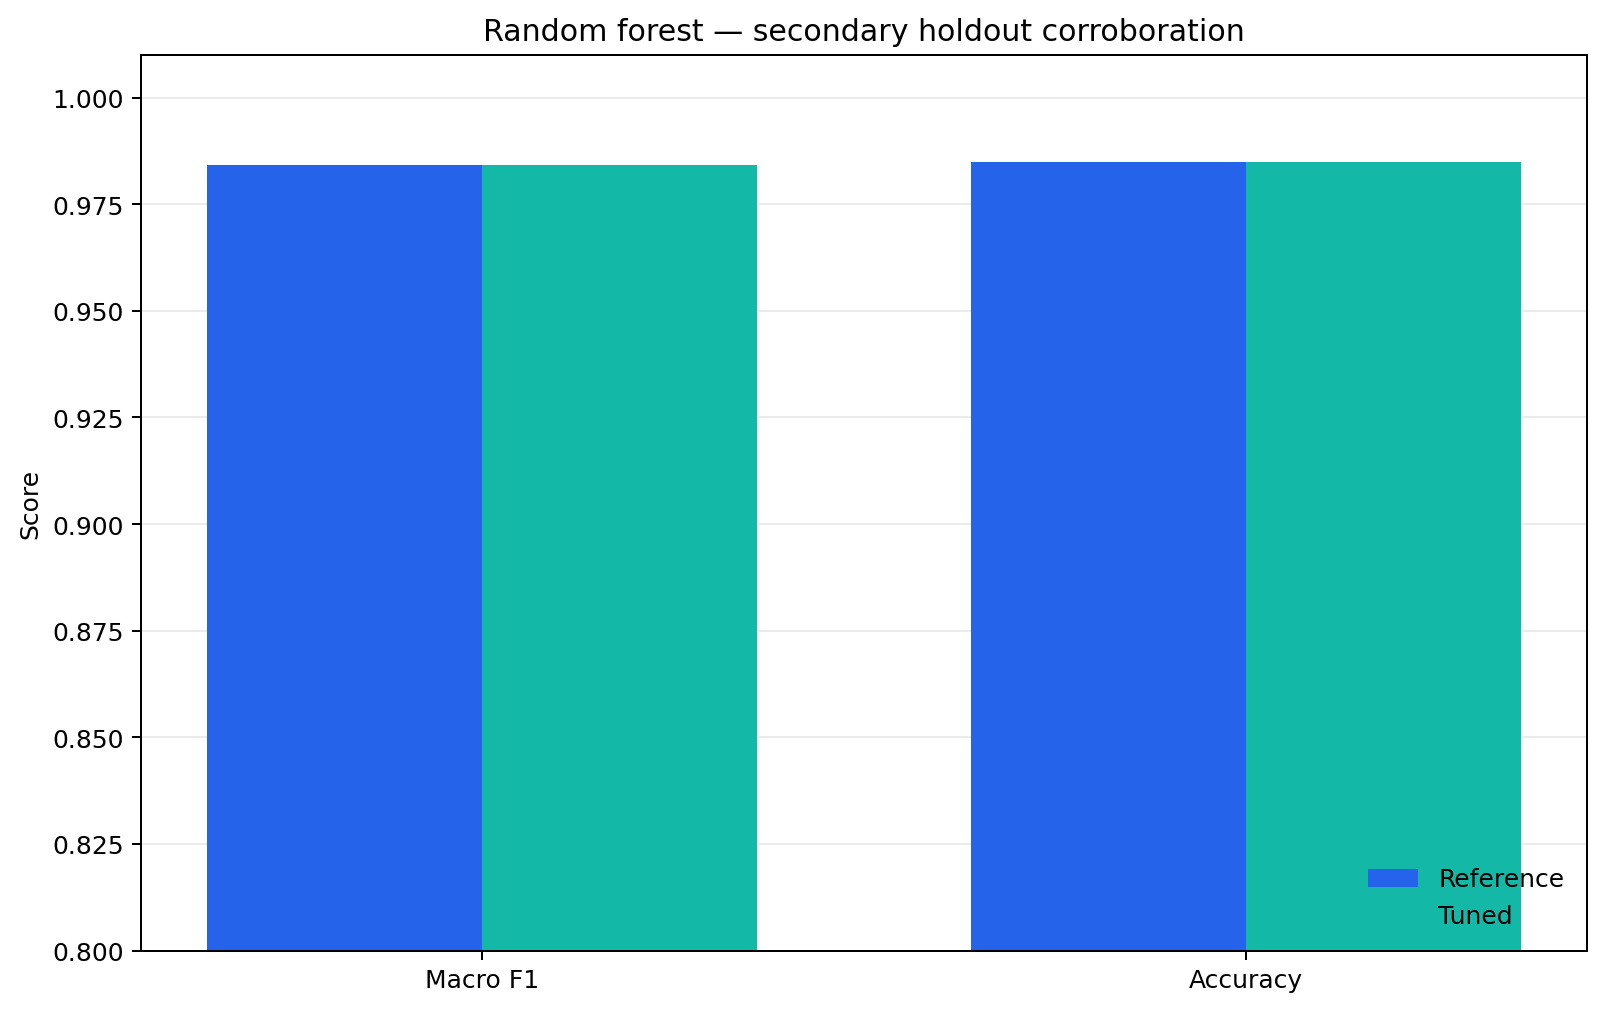
\includegraphics[width=\textwidth]{../figures/en/fig_rf_corroboration_holdout.png}
\caption{Secondary comparison between the reference and \texttt{tuned} random-forest variants on the corroboration set.}
\end{figure}

% --- DECISION TREE ---
\subsection{Decision tree model}

\subsubsection{Role of the model}
The decision tree is studied here less as a final candidate than as a reference point for the tradeoff between interpretability and generalization. This family makes the effects of depth, leaf size, and pruning directly observable, but is also particularly prone to overfitting in a rich multiclass problem.

\subsubsection{Exploration}
The two exploratory variants clearly bracket the family's behavior. The \texttt{default} variant achieves \texttt{0.5809} in \texttt{F1-macro} and \texttt{0.6174} in \texttt{accuracy}, but with a very high generalization gap (\texttt{0.4191}). Conversely, \texttt{restricted\_depth} sharply reduces this gap (\texttt{0.0797}) at the cost of a collapse in performance, reaching only \texttt{0.1468} in \texttt{F1-macro}.

\begin{table}[H]
\centering
\begin{tabular}{|l|l|r|r|r|r|}
\hline
\textbf{Variant} & \textbf{Protocol} & \textbf{Macro F1} & \textbf{Accuracy} & \textbf{F1 gap} & \textbf{Time (s)} \\
\hline
\texttt{default} & simple CV & \texttt{0.5809} & \texttt{0.6174} & \texttt{0.4191} & \texttt{1.04} \\
\texttt{restricted\_depth} & simple CV & \texttt{0.1468} & \texttt{0.1529} & \texttt{0.0797} & \texttt{0.56} \\
\hline
\end{tabular}
\end{table}

The exploratory conclusion is unambiguous: an overly flexible tree memorizes the data, while an overly constrained tree loses most of its discriminative power. A useful region exists for the family, but it appears narrow and unstable.

\begin{figure}[H]
\centering
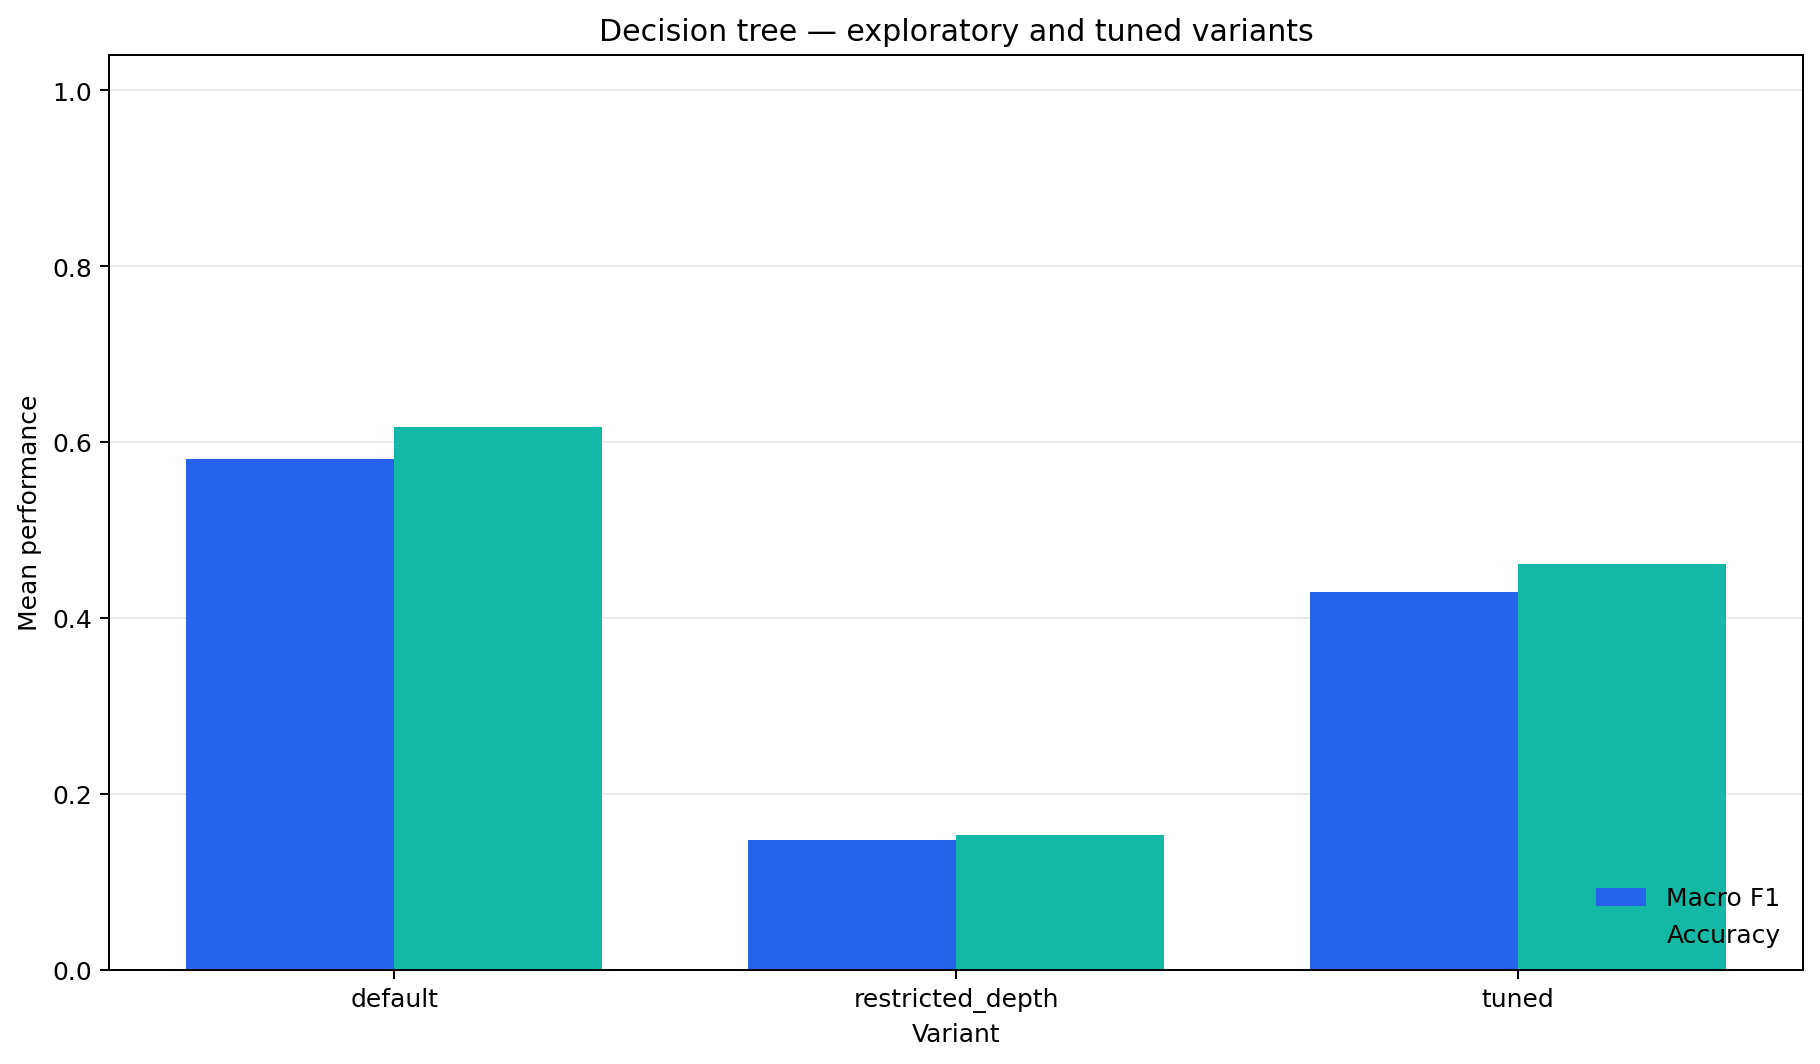
\includegraphics[width=\textwidth]{../figures/en/fig_dt_comparaison_variantes.png}
\caption{Exploratory comparison of decision-tree variants. The performance--complexity tradeoff remains generally unfavorable for a single tree.}
\end{figure}

\subsubsection{Confirmation}
Nested cross-validation confirms this fragility. The \texttt{tuned} variant achieves a mean \texttt{F1-macro} of \texttt{0.4295} and mean \texttt{accuracy} of \texttt{0.4610}, with standard deviations of \texttt{0.0546} and \texttt{0.0627}. The decline relative to the \texttt{default} variant does not mean that tuning degrades the model; rather, it indicates that a stricter confirmatory estimate corrects the optimism of simple evaluation for a highly unstable estimator.

\begin{table}[H]
\centering
\begin{tabular}{|l|r|}
\hline
\textbf{Confirmatory metric} & \textbf{Value} \\
\hline
Mean Macro F1 & \texttt{0.4295} \\
F1 standard deviation & \texttt{0.0546} \\
Mean accuracy & \texttt{0.4610} \\
Accuracy standard deviation & \texttt{0.0627} \\
Protocol & \texttt{nested CV} \\
Outer folds & \texttt{5} \\
Inner folds & \texttt{3} \\
Total time (s) & \texttt{11.47} \\
\hline
\end{tabular}
\end{table}

The decision tree therefore ranks far behind the other families. It remains pedagogically useful for examining the mechanisms of overfitting, but it is not a competitive solution in this project.

\subsubsection{Descriptive diagnostics}
The validation curve for \texttt{max\_depth} directly exposes the core problem: the training score rises quickly with depth, whereas the validation score plateaus and then deteriorates. Accordingly, the confusion matrices show a much more diffuse pattern than those of the best-performing models.

\begin{figure}[H]
\centering
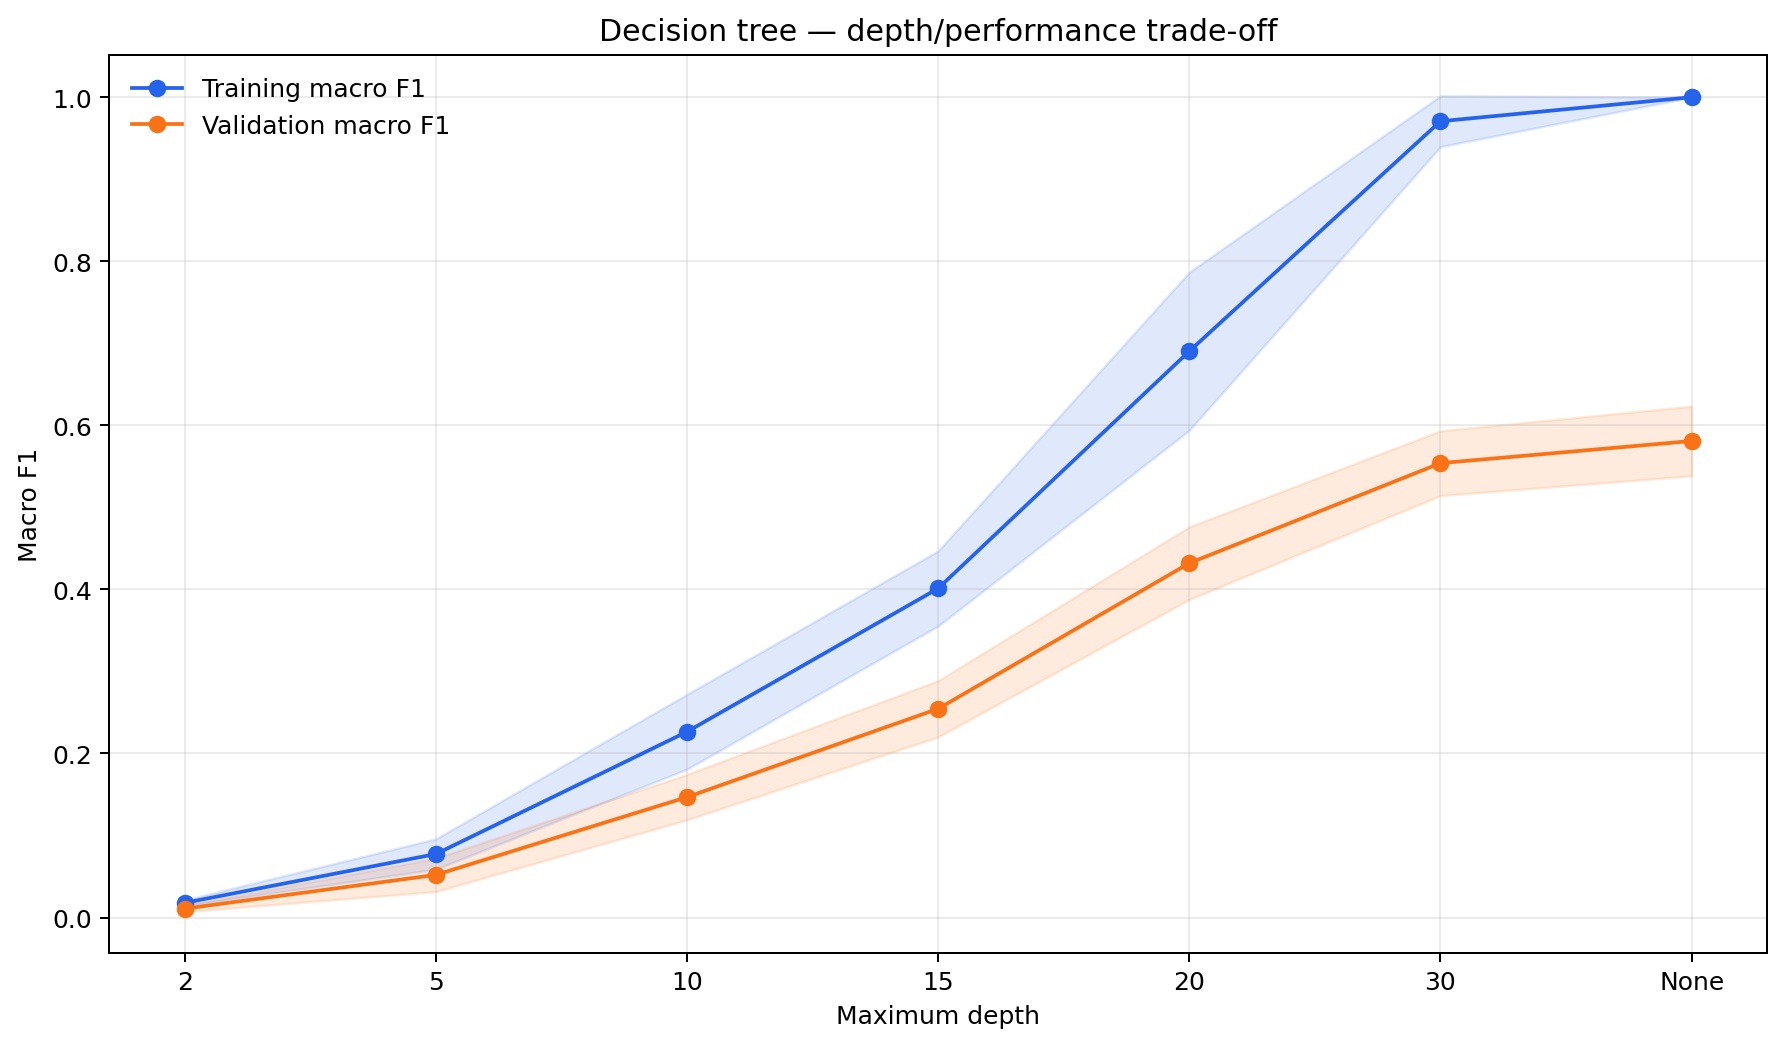
\includegraphics[width=\textwidth]{../figures/en/figA3_validation_curve_max_depth.png}
\caption{Exploratory validation curve for \texttt{max\_depth}. The divergence between training and validation directly illustrates the family's fragility.}
\end{figure}

\begin{figure}[H]
\centering
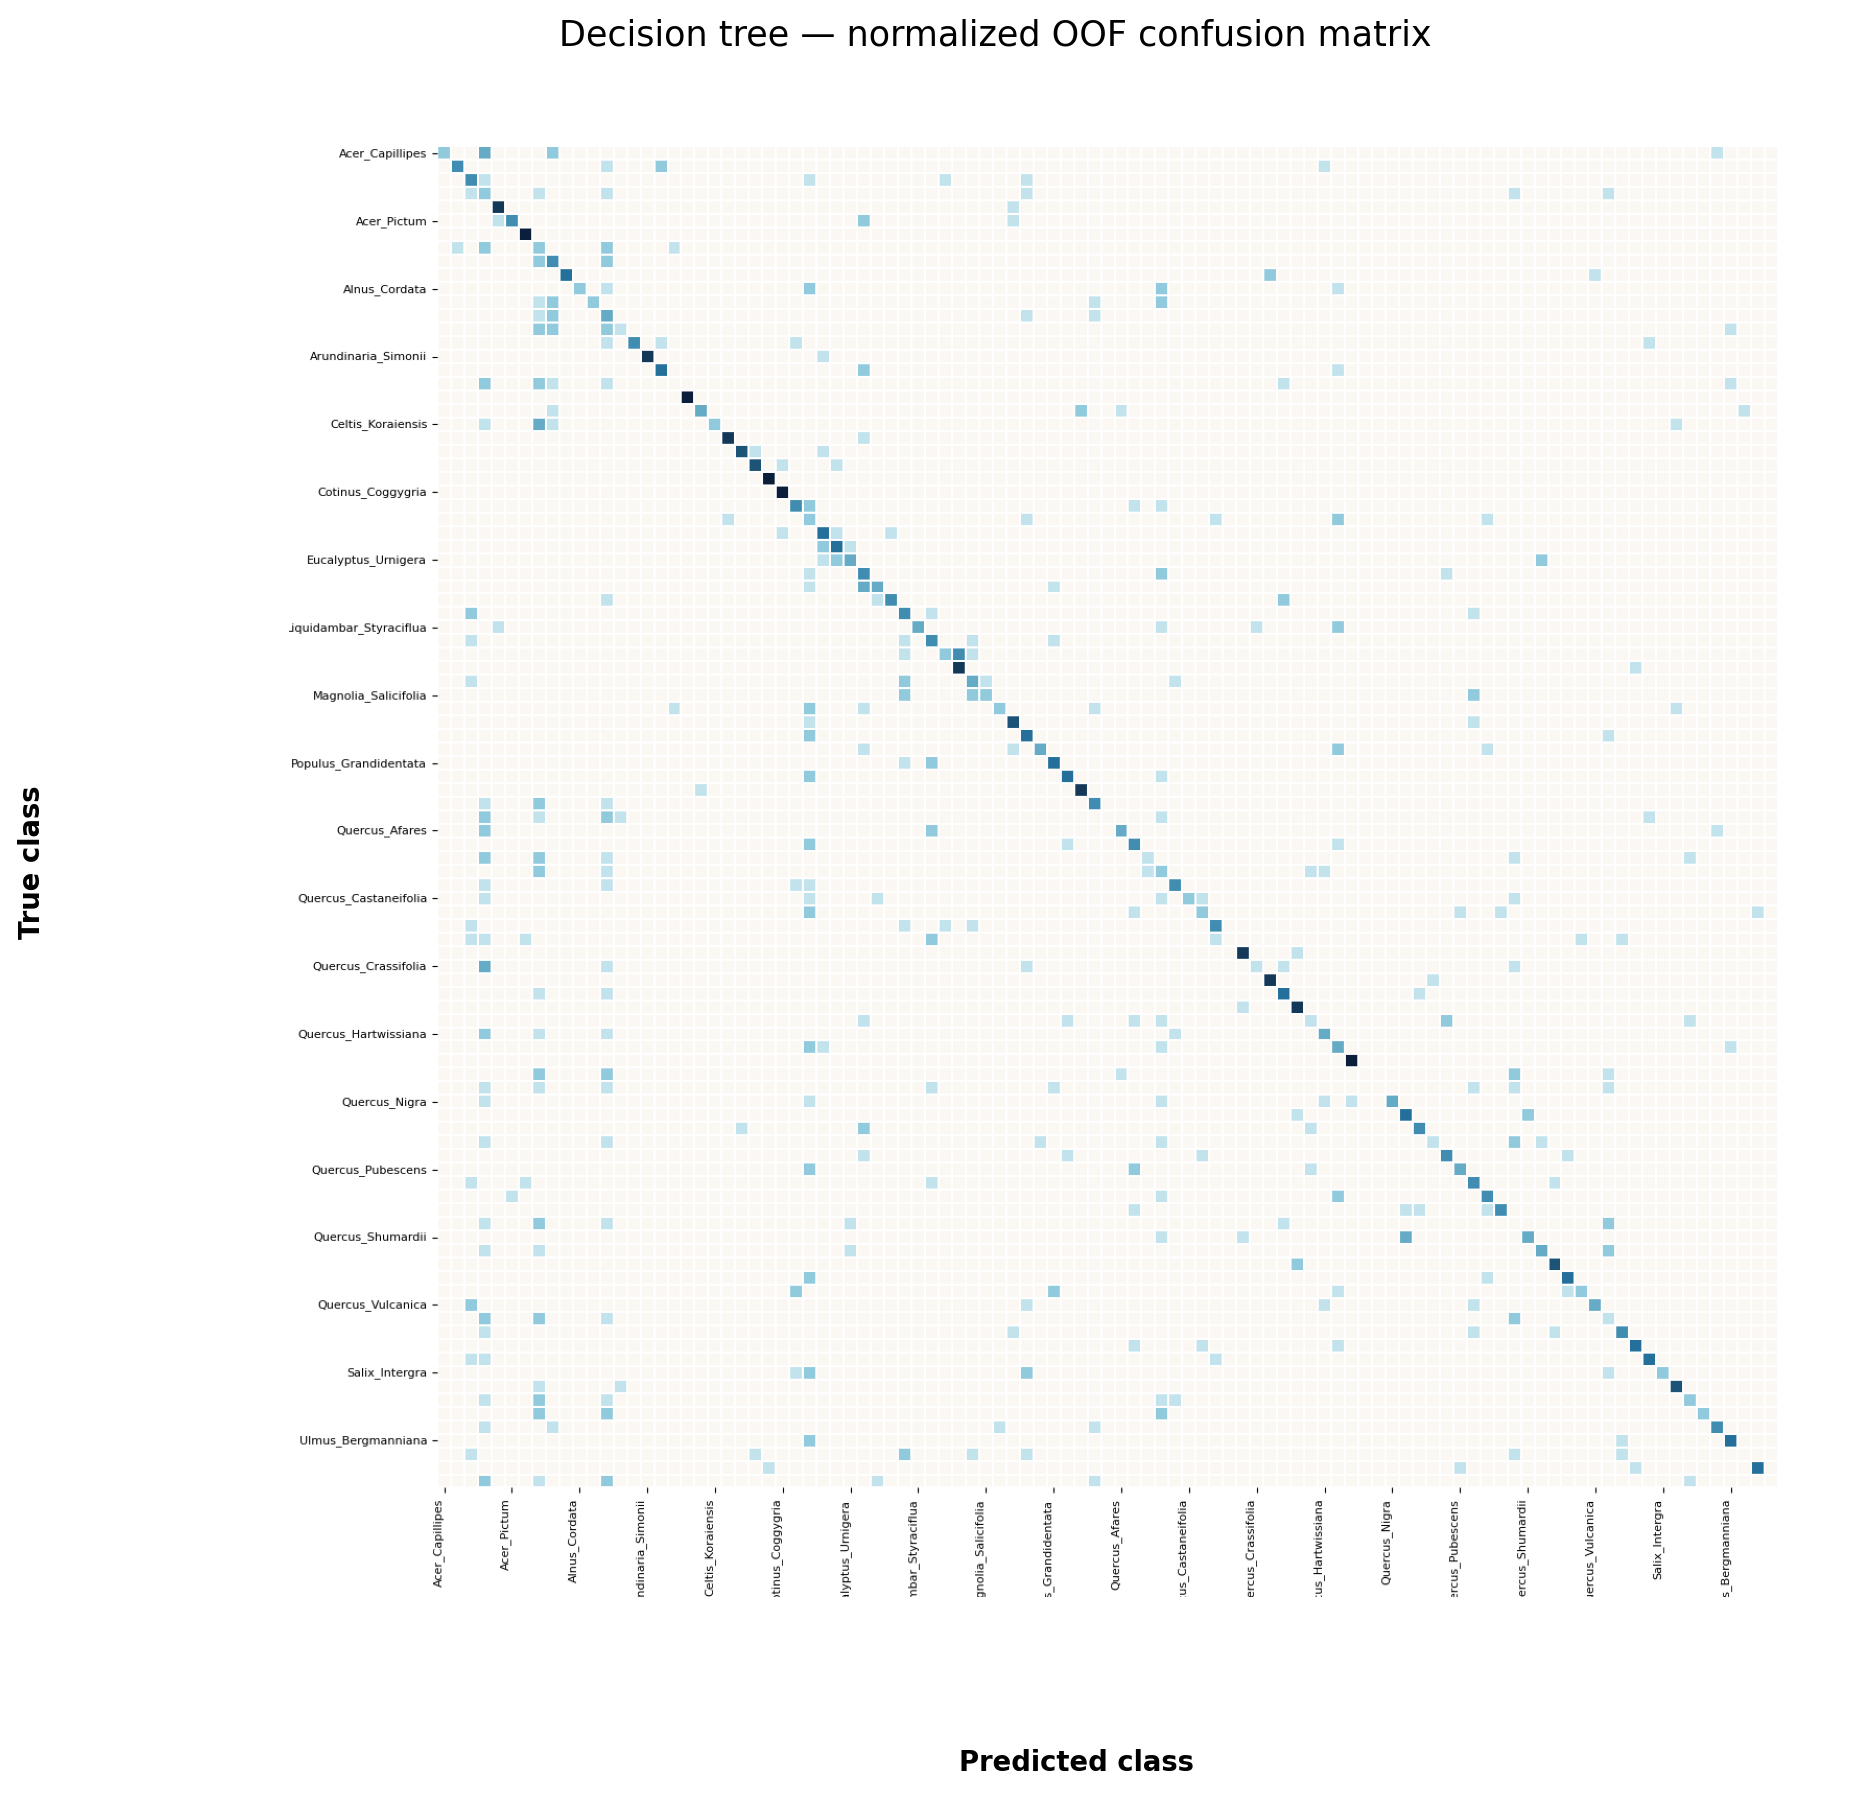
\includegraphics[width=\textwidth]{../figures/en/figA_confusion_dt_tuned.png}
\caption{Normalized confusion matrix from the out-of-fold predictions of the \texttt{tuned} variant. Errors remain numerous and dispersed.}
\end{figure}

\begin{figure}[H]
\centering
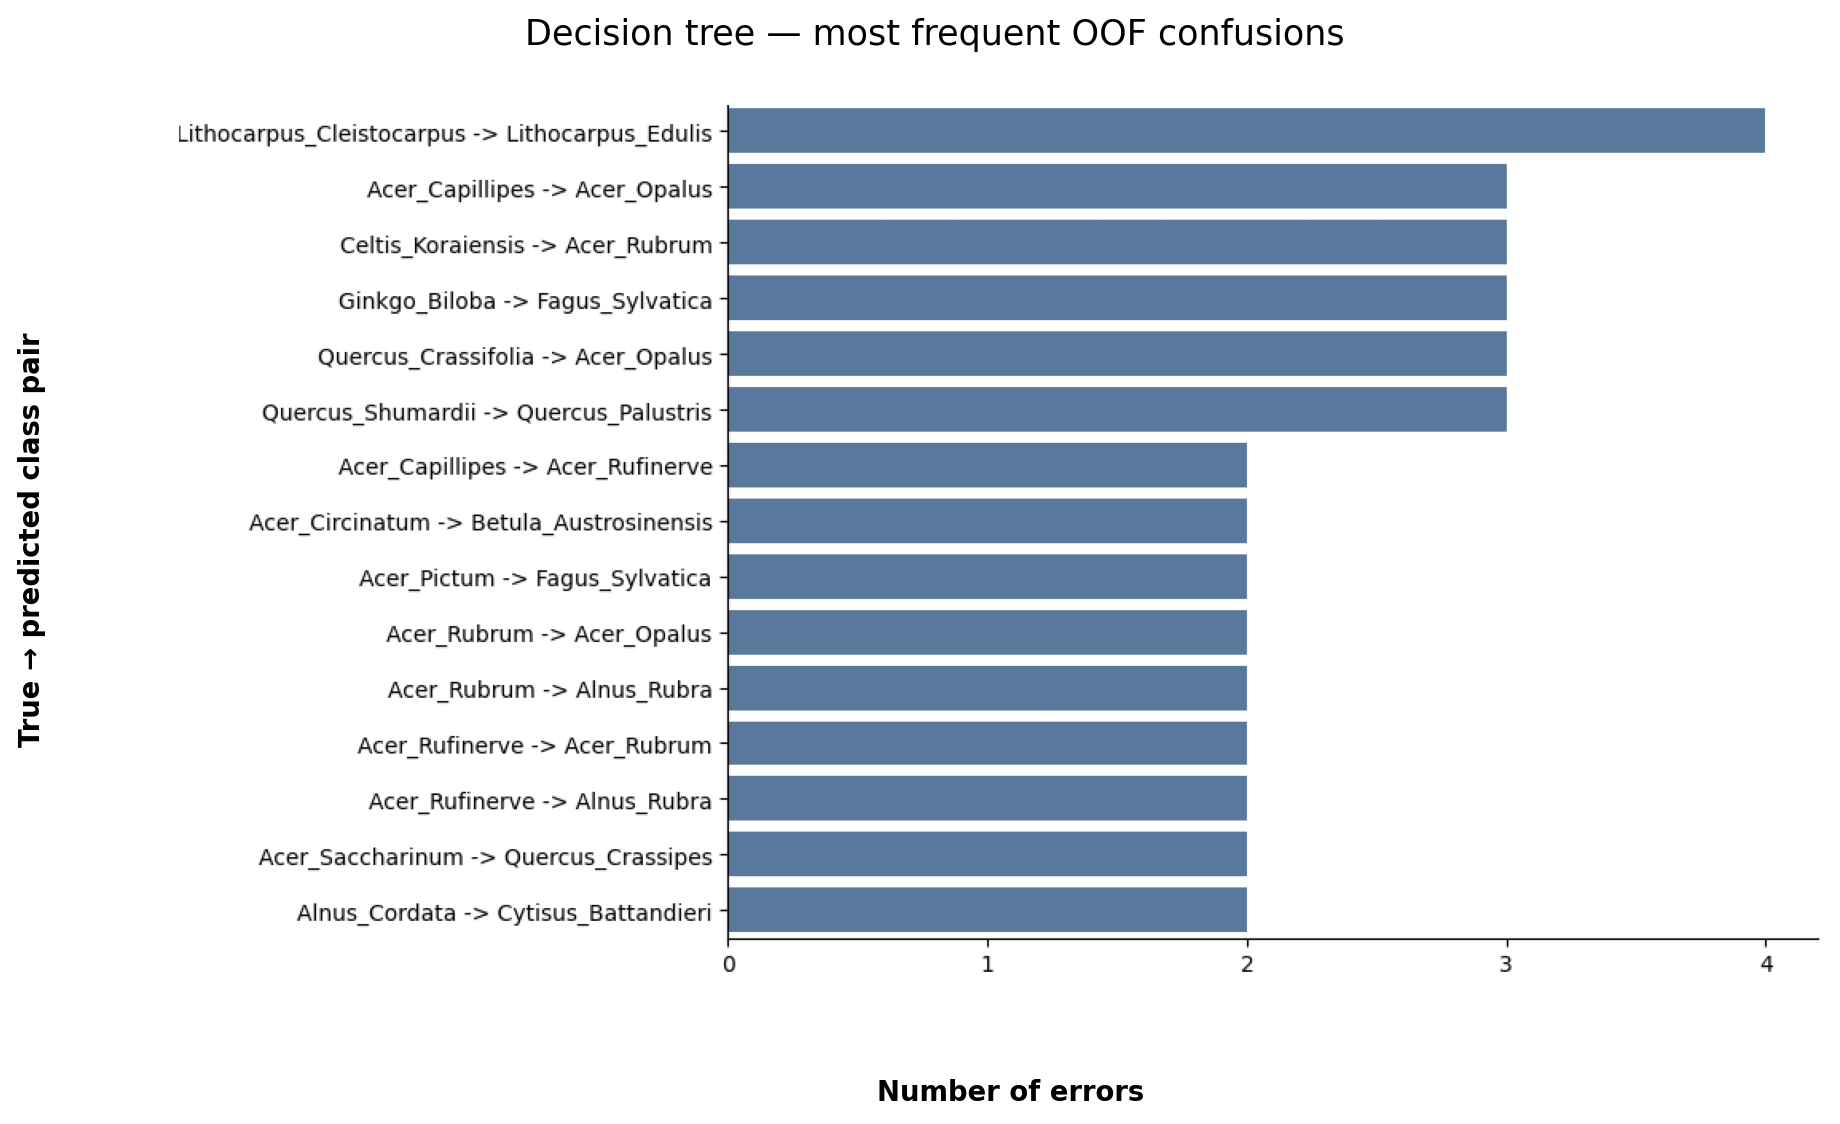
\includegraphics[width=\textwidth]{../figures/en/fig_dt_top12_confusions.png}
\caption{Leading confusions for the tuned decision tree. Their dispersion is consistent with insufficient generalization on a problem with \texttt{99} classes.}
\end{figure}

\subsubsection{No secondary corroboration}
Unlike the other eligible families, no secondary corroboration is published for the decision tree in the canonical artifacts. The scientific interpretation therefore rests solely on the relationship among exploration, confirmation, and confusion diagnostics.

This absence does not change the substantive conclusion. Even without secondary corroboration, the confirmatory results are sufficient to show that a single tree remains too unstable to compete with regularized linear models, the SVM, the random forest, or even the MLP.

% --- MLP ---
\subsection{MLP model}

\subsubsection{Role of the model}
The MLP represents the study's dense neural-network family. It tests whether a nonlinear capacity more flexible than linear or kernel models produces an empirical gain on a moderately sized tabular dataset with relatively few examples per class.

\subsubsection{Exploration}
The exploratory stage shows very clearly that preprocessing is a prerequisite for this model to function effectively. Without scaling, the MLP collapses to \texttt{0.1642} in \texttt{F1-macro} and \texttt{0.1863} in \texttt{accuracy}, with very high variability. Once the variables are standardized, the \texttt{scaled\_only} variant reaches \texttt{0.9389} in \texttt{F1-macro} and \texttt{0.9482} in \texttt{accuracy}, while \texttt{scaled\_pca} reaches \texttt{0.9323} and \texttt{0.9444}.

\begin{table}[H]
\centering
\begin{tabular}{|l|l|r|r|r|r|}
\hline
\textbf{Variant} & \textbf{Protocol} & \textbf{Macro F1} & \textbf{Accuracy} & \textbf{F1 gap} & \textbf{Time (s)} \\
\hline
\texttt{default} & simple CV & \texttt{0.1642} & \texttt{0.1863} & \texttt{0.0262} & \texttt{1.97} \\
\texttt{scaled\_only} & simple CV & \texttt{0.9389} & \texttt{0.9482} & \texttt{0.0552} & \texttt{2.01} \\
\texttt{scaled\_pca} & simple CV & \texttt{0.9323} & \texttt{0.9444} & \texttt{0.0604} & \texttt{1.97} \\
\hline
\end{tabular}
\end{table}

The central diagnosis is therefore clear: the MLP becomes competitive only when supplied through a strict standardization pipeline. \texttt{PCA} provides no clear benefit and remains slightly behind the \texttt{scaled\_only} variant.

\begin{figure}[H]
\centering
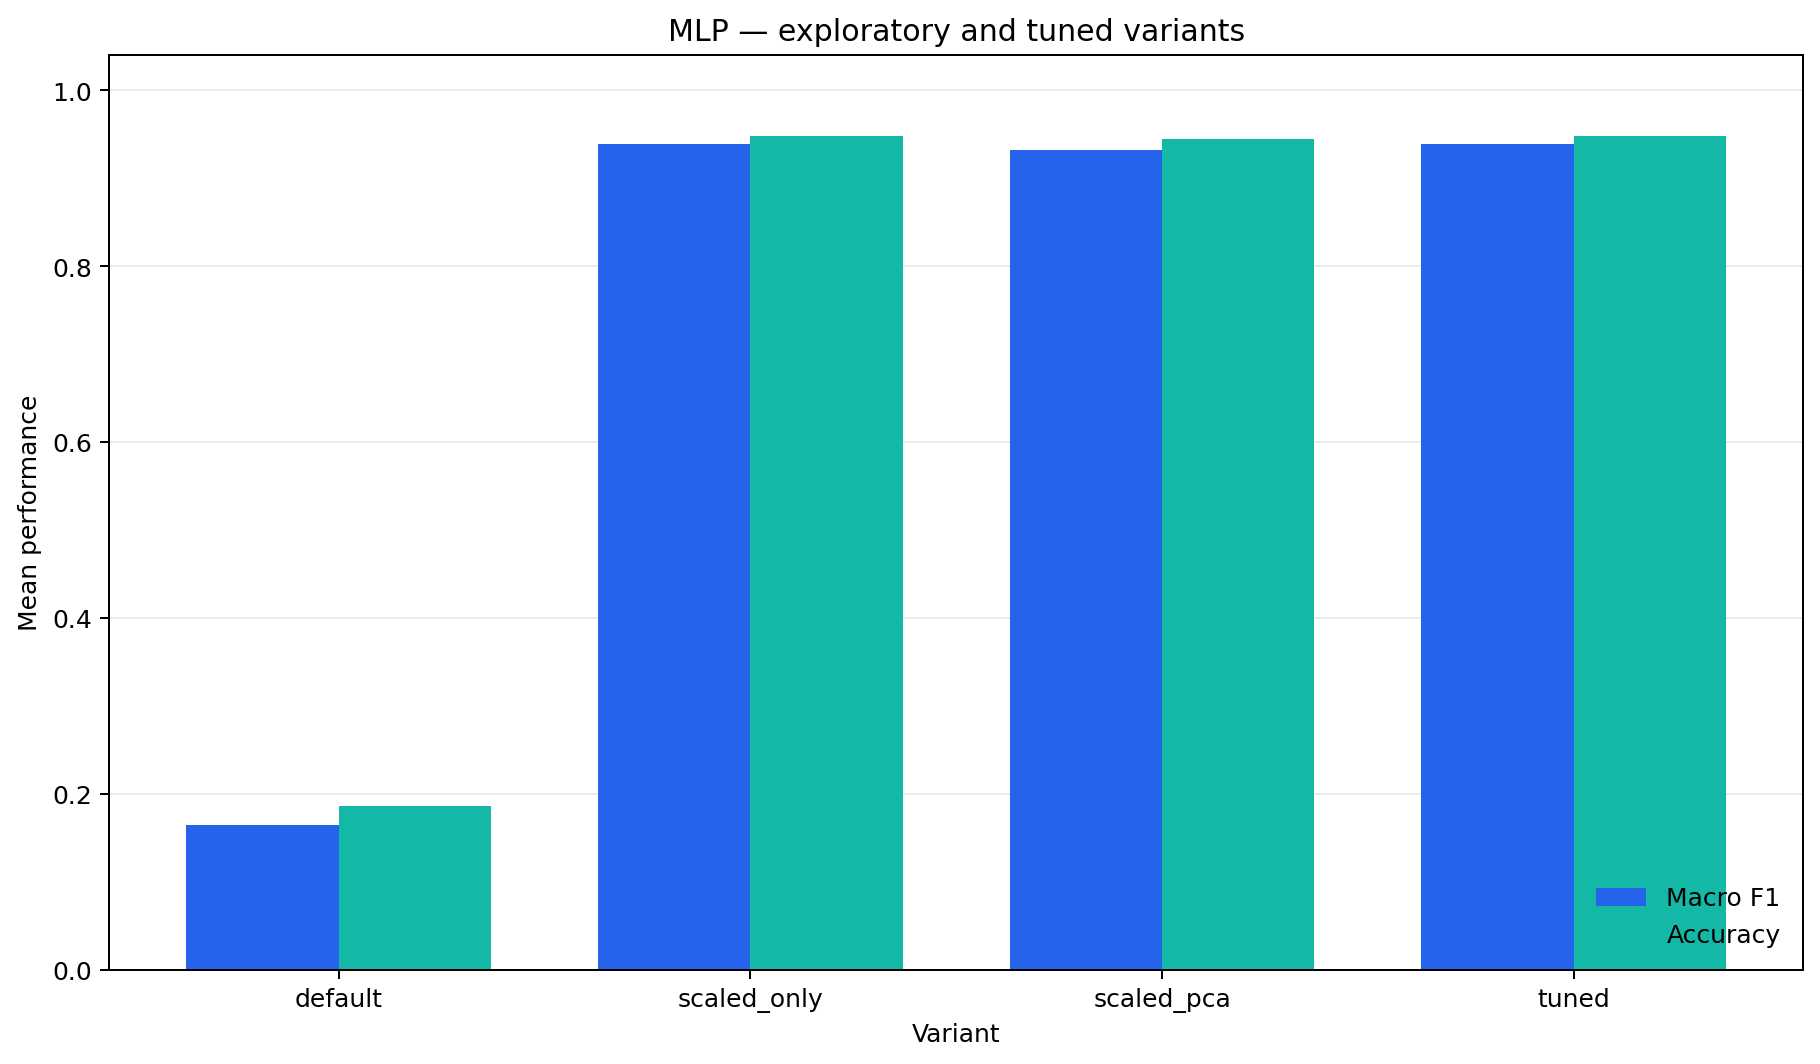
\includegraphics[width=\textwidth]{../figures/en/fig_mlp_comparaison_variantes.png}
\caption{Exploratory comparison of MLP variants. The contrast between the raw and scaled versions illustrates the network's dependence on feature scale.}
\end{figure}

\subsubsection{Confirmation}
Confirmatory evaluation yields a mean \texttt{F1-macro} of \texttt{0.9389} and mean \texttt{accuracy} of \texttt{0.9482}, with standard deviations of \texttt{0.0322} and \texttt{0.0279}. The \texttt{tuned} variant therefore reproduces the best exploratory result almost exactly, suggesting that tuning confirms an already strong configuration rather than providing a substantial gain.

\begin{table}[H]
\centering
\begin{tabular}{|l|r|}
\hline
\textbf{Confirmatory metric} & \textbf{Value} \\
\hline
Mean Macro F1 & \texttt{0.9389} \\
F1 standard deviation & \texttt{0.0322} \\
Mean accuracy & \texttt{0.9482} \\
Accuracy standard deviation & \texttt{0.0279} \\
Protocol & \texttt{nested CV} \\
Outer folds & \texttt{5} \\
Inner folds & \texttt{3} \\
Total time (s) & \texttt{38.25} \\
\hline
\end{tabular}
\end{table}

The MLP thus ranks fourth in the confirmatory comparison. It remains clearly effective, but does not convert its additional flexibility into an advantage over the leading trio of logistic regression, SVM, and random forest.

\subsubsection{Descriptive diagnostics}
The diagnostics associated with the MLP primarily clarify its optimization dynamics. The loss curve indicates proper convergence, while the exploratory tuning table shows that most of the signal comes from hidden-layer size rather than \texttt{alpha}. The \texttt{(128,)} configuration consistently outperforms \texttt{(64,)}, while \texttt{PCA} remains slightly behind. These diagnostics help explain the model's behavior without competing with the confirmatory metrics.

\begin{figure}[H]
\centering
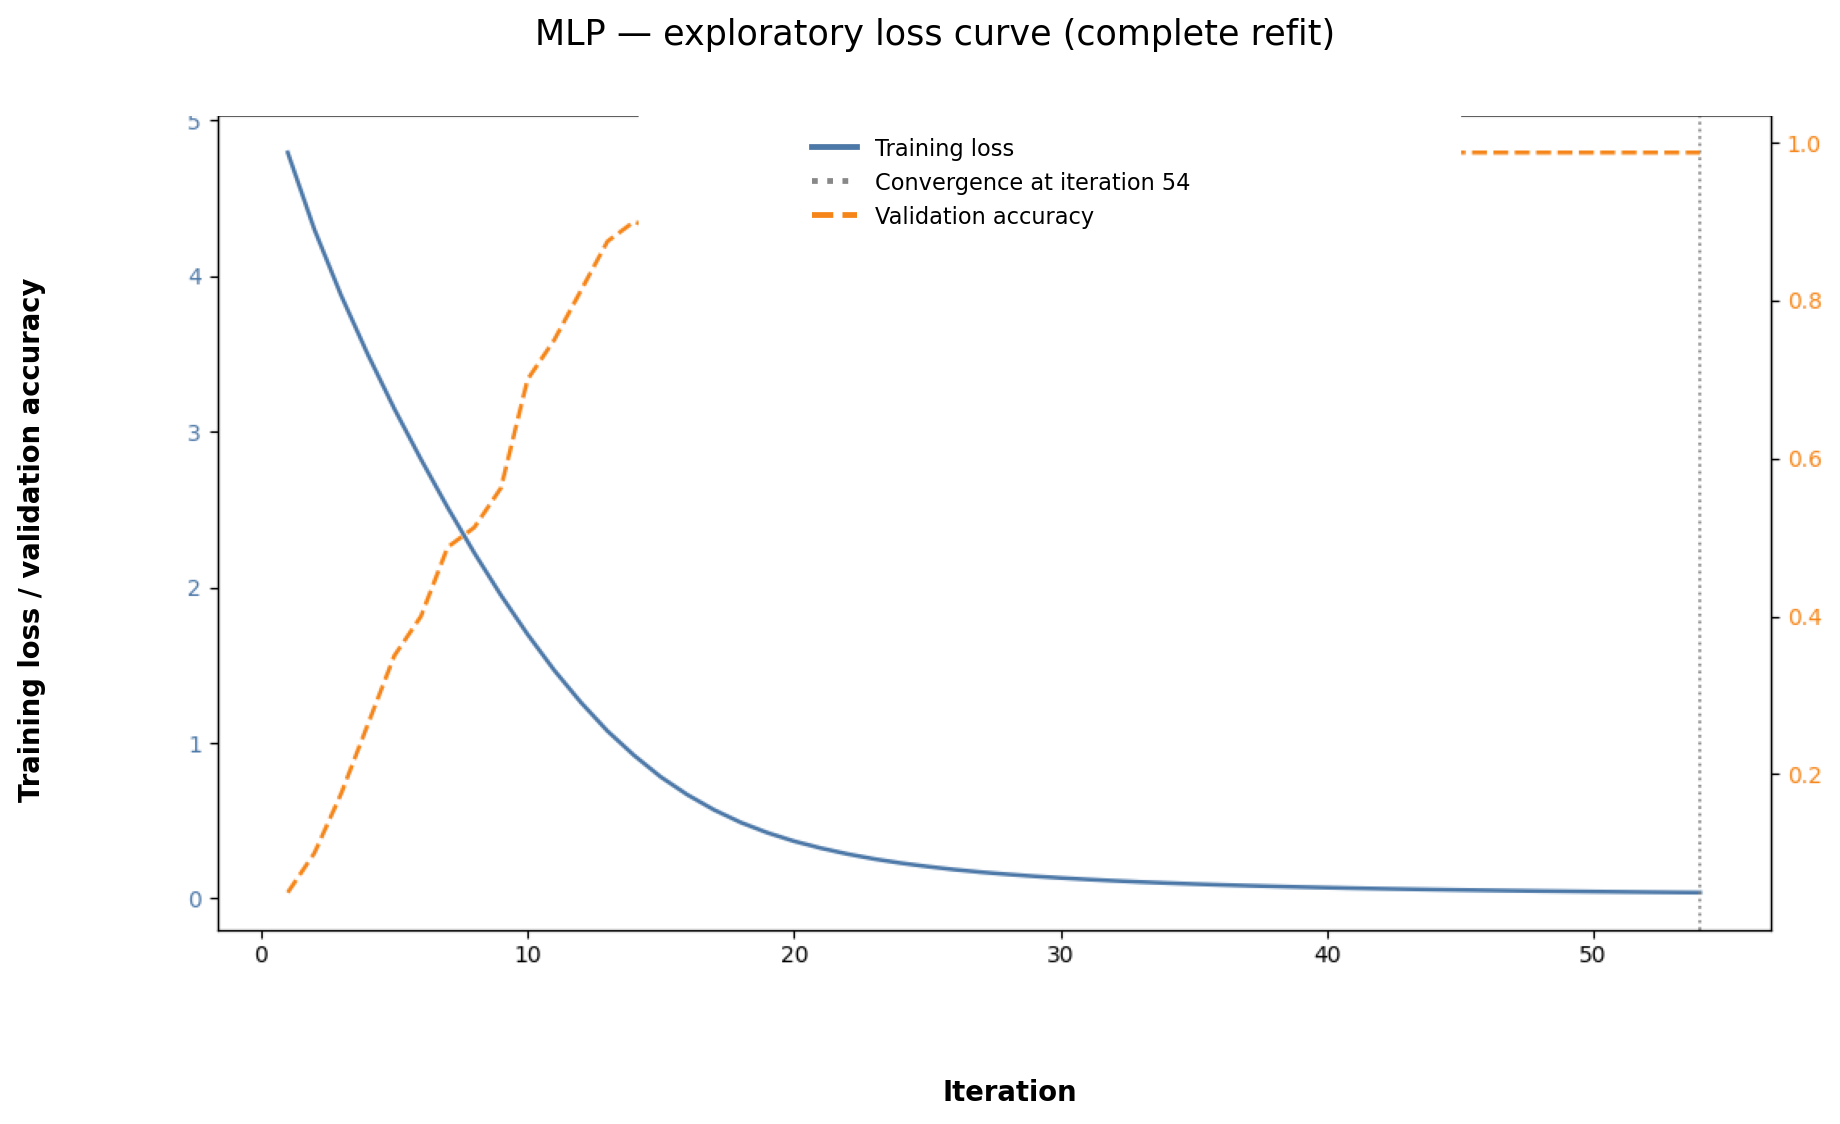
\includegraphics[width=\textwidth]{../figures/en/figA5_loss_curve.png}
\caption{Exploratory diagnostic of MLP convergence. The loss stabilizes properly, although this evidence remains descriptive.}
\end{figure}

\begin{table}[H]
\centering
\begin{tabular}{|l|r|r|}
\hline
\textbf{hidden\_layer\_sizes / alpha} & \textbf{0.0001} & \textbf{0.0010} \\
\hline
\texttt{(64,)} & \texttt{0.9055} & \texttt{0.9055} \\
\texttt{(128,)} & \texttt{0.9341} & \texttt{0.9341} \\
\hline
\end{tabular}
\caption{Exploratory MLP tuning without PCA (mean CV \texttt{F1-macro})}
\end{table}

\begin{table}[H]
\centering
\begin{tabular}{|l|r|r|}
\hline
\textbf{hidden\_layer\_sizes / alpha} & \textbf{0.0001} & \textbf{0.0010} \\
\hline
\texttt{(64,)} & \texttt{0.9107} & \texttt{0.9107} \\
\texttt{(128,)} & \texttt{0.9266} & \texttt{0.9266} \\
\hline
\end{tabular}
\caption{Exploratory MLP tuning with PCA (mean CV \texttt{F1-macro})}
\end{table}

\begin{figure}[H]
\centering
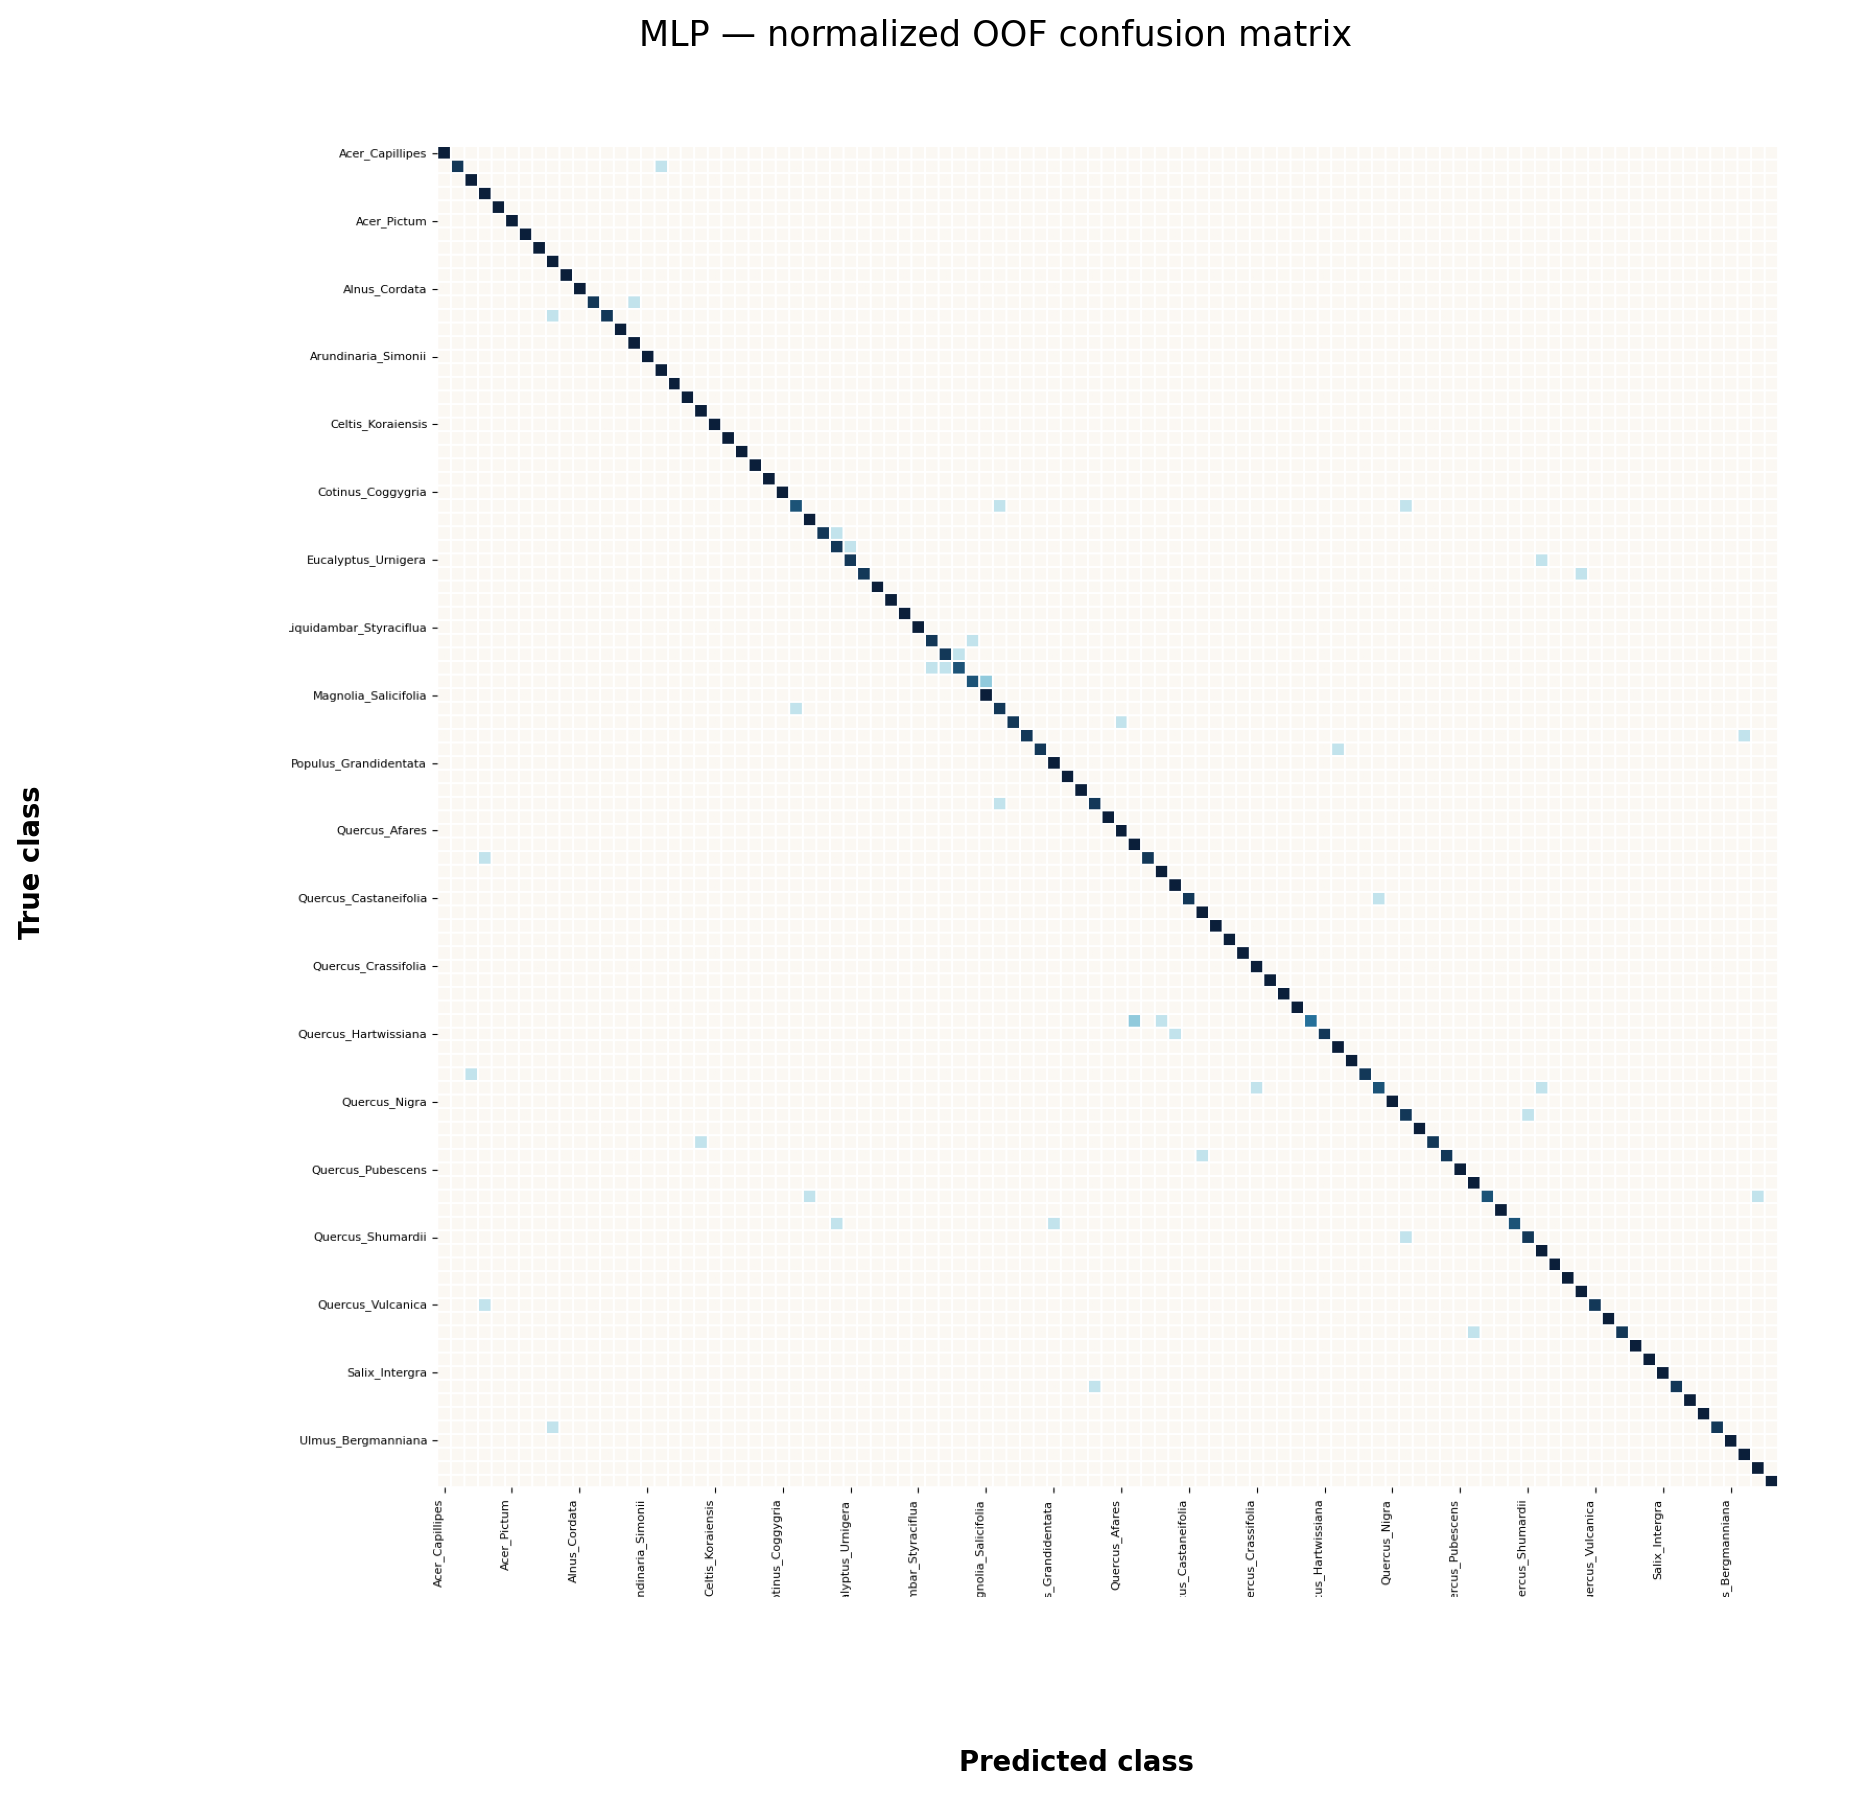
\includegraphics[width=\textwidth]{../figures/en/figA_confusion_mlp_tuned.png}
\caption{Normalized confusion matrix from the out-of-fold predictions of the \texttt{tuned} variant. Residual errors remain limited, but are more numerous than for the three best-performing families.}
\end{figure}

\begin{figure}[H]
\centering
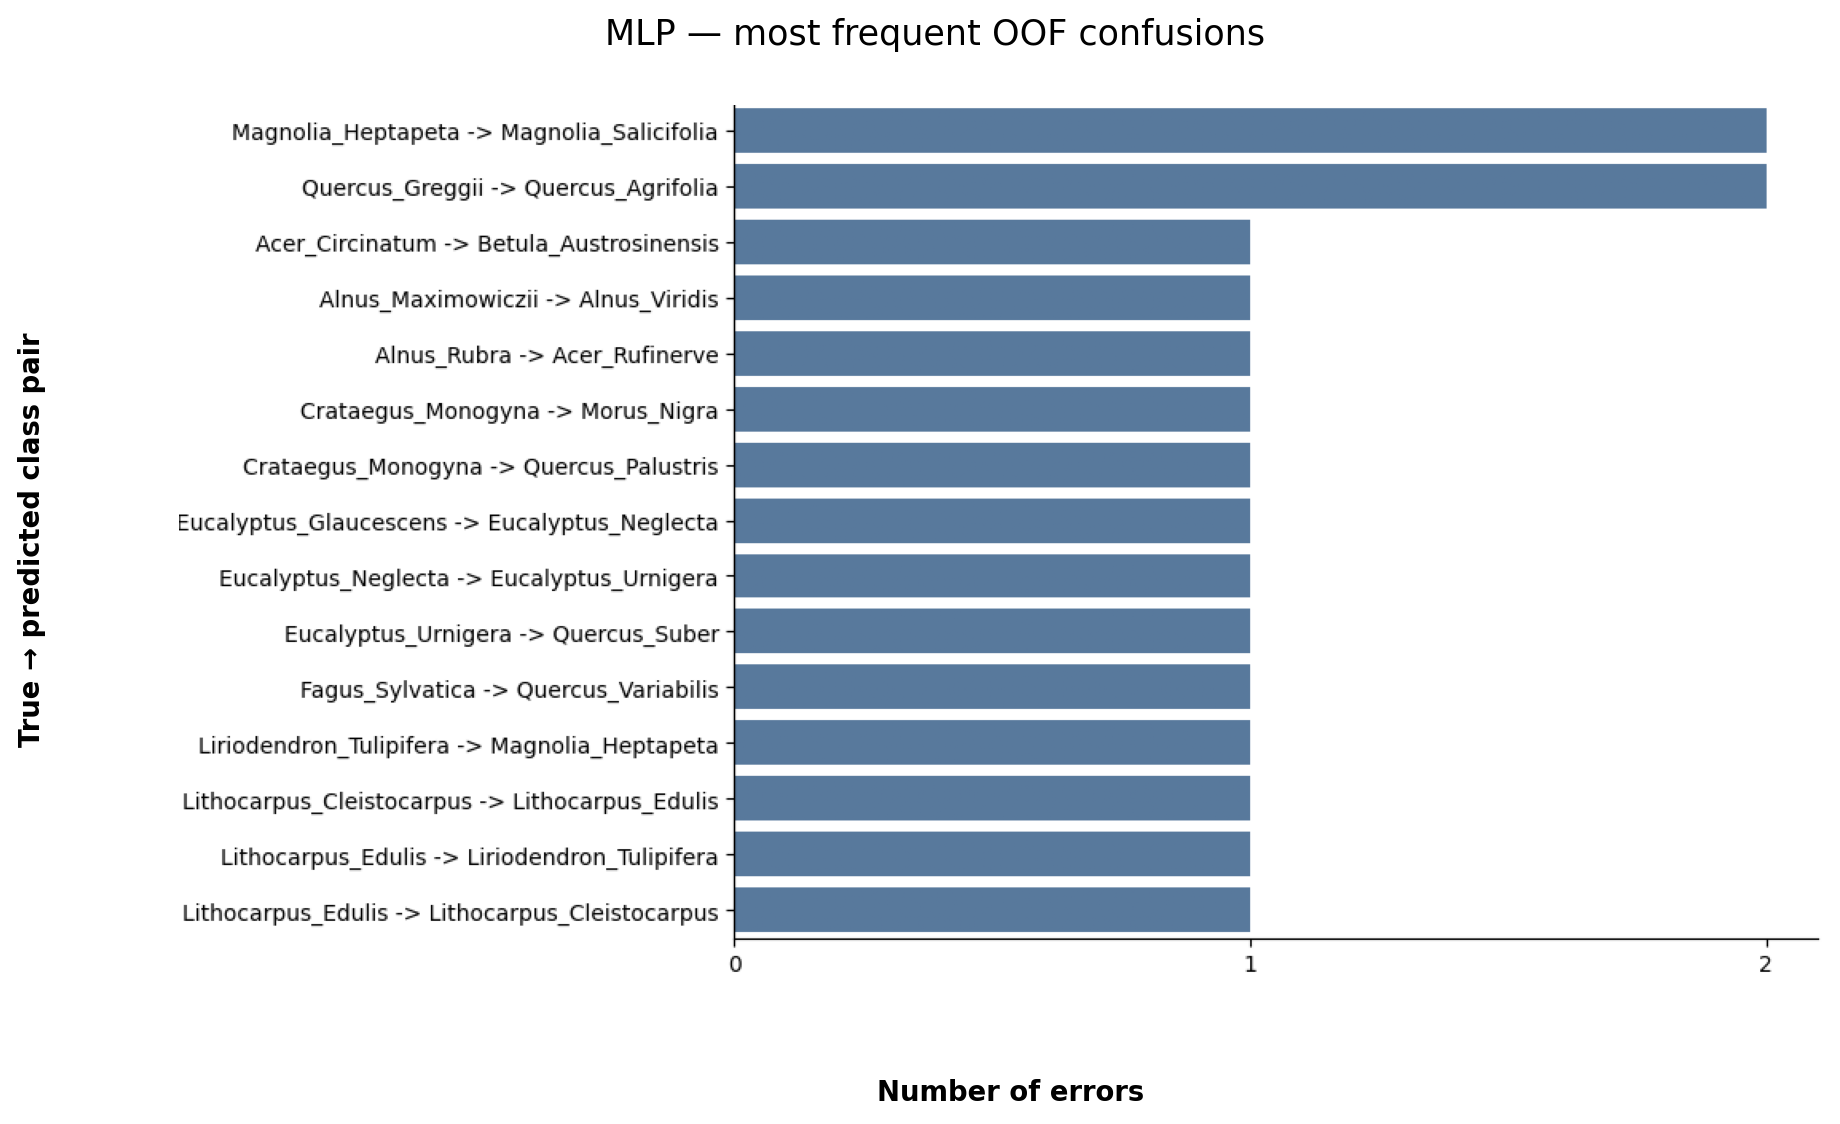
\includegraphics[width=\textwidth]{../figures/en/fig_mlp_top12_confusions.png}
\caption{Leading confusions for the tuned MLP. They remain relatively concentrated and confirm an overall competitive performance level.}
\end{figure}

\subsubsection{Secondary corroboration}
The frozen corroboration set retains \texttt{scaled\_only} as the secondary reference. On this split, the reference and \texttt{tuned} variants obtain exactly the same scores: \texttt{0.9785} in \texttt{F1-macro} and \texttt{0.9798} in \texttt{accuracy}. The \texttt{scaled\_pca} variant remains slightly behind. The \texttt{tuned - reference} delta is therefore zero.

\begin{table}[H]
\centering
\begin{tabular}{|l|r|r|l|}
\hline
\textbf{Variant} & \textbf{Corroboration F1} & \textbf{Corroboration accuracy} & \textbf{Role} \\
\hline
\texttt{default} & \texttt{0.0080} & \texttt{0.0404} & baseline \\
\texttt{scaled\_only} & \texttt{0.9785} & \texttt{0.9798} & reference \\
\texttt{scaled\_pca} & \texttt{0.9737} & \texttt{0.9747} & descriptive \\
\texttt{tuned} & \texttt{0.9785} & \texttt{0.9798} & tuned \\
\hline
\end{tabular}
\end{table}

The conclusion for the MLP remains straightforward: with appropriate preprocessing, the family becomes strong, but tuning adds no robust gain on this dataset. It remains credible without surpassing the best, more parsimonious options.

\begin{figure}[H]
\centering
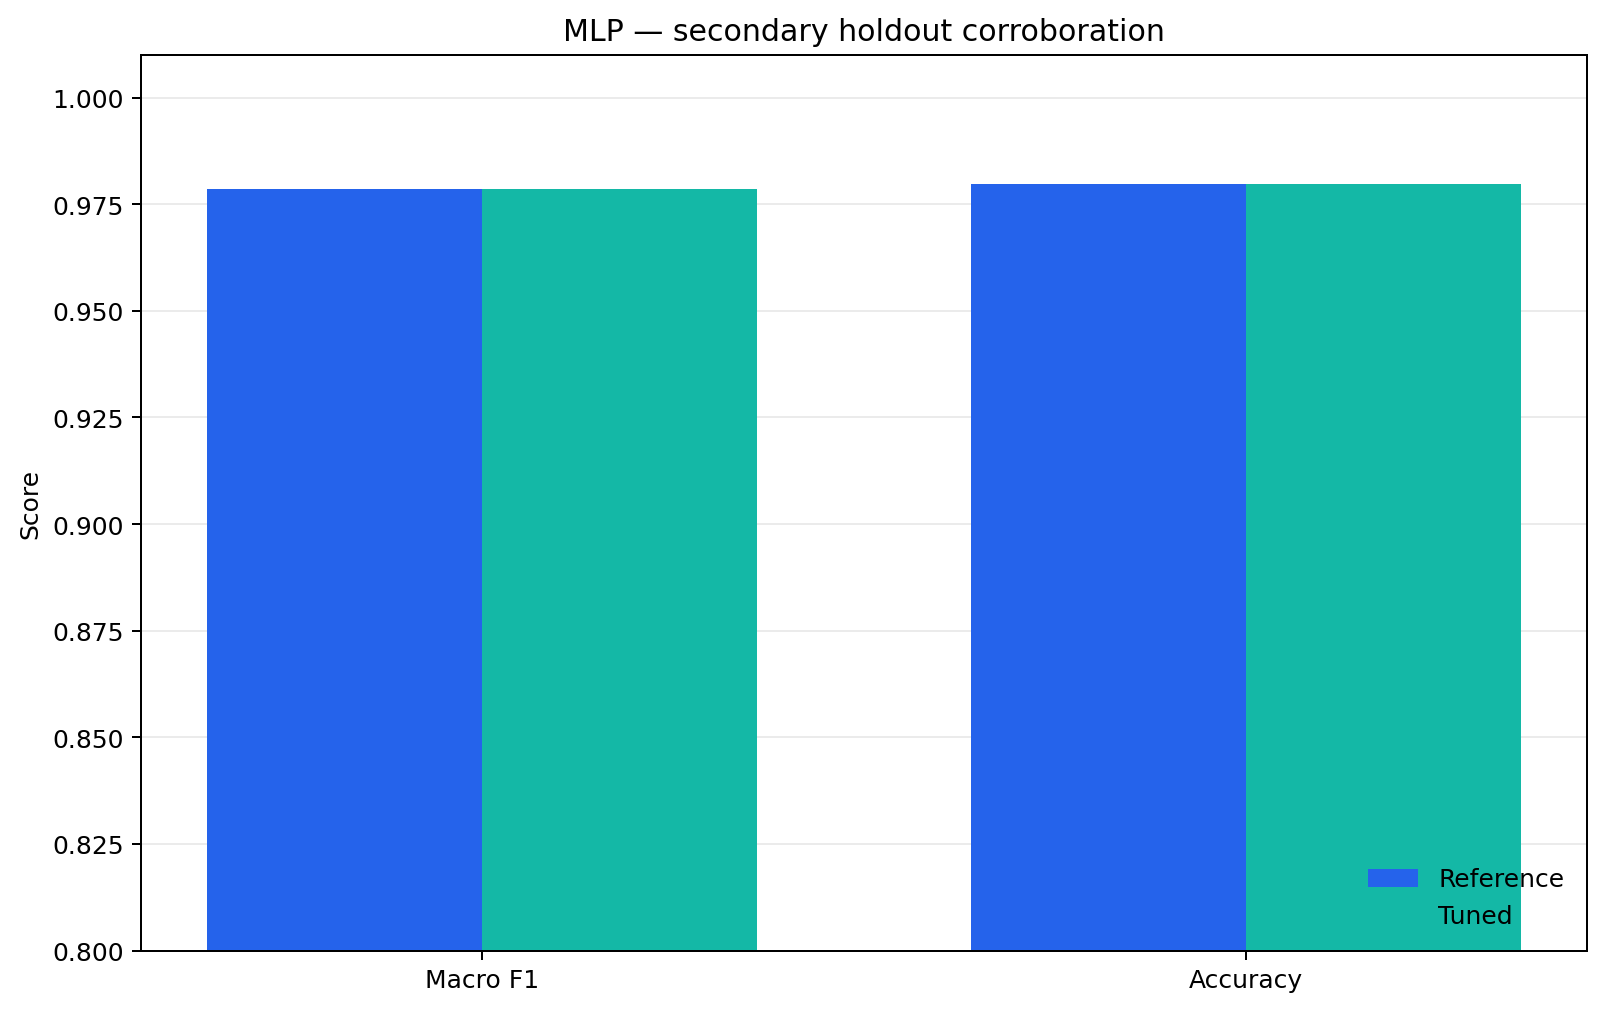
\includegraphics[width=\textwidth]{../figures/en/fig_mlp_corroboration_holdout.png}
\caption{Secondary comparison between the reference and \texttt{tuned} MLP variants on the corroboration set.}
\end{figure}

% ==========================================
% 4. OVERALL COMPARISON AND DISCUSSION
% ==========================================
